\documentclass[a4paper,11pt]{book}
%\documentclass[a4paper,twoside,11pt,titlepage]{book}
\usepackage{listings}
\usepackage[utf8]{inputenc}
\usepackage[spanish,es-tabla]{babel}
\usepackage{amsmath}
\usepackage{esvect}


% \usepackage[style=list, number=none]{glossary} %
%\usepackage{titlesec}
%\usepackage{pailatino}

\decimalpoint
\usepackage{dcolumn}
\newcolumntype{.}{D{.}{\esperiod}{-1}}
\makeatletter
\addto\shorthandsspanish{\let\esperiod\es@period@code}
\makeatother


%\usepackage[chapter]{algorithm}
\RequirePackage{verbatim}
%\RequirePackage[Glenn]{fncychap}
\usepackage{fancyhdr}
\usepackage{graphicx}
\usepackage{afterpage}

\usepackage{longtable}

\usepackage[pdfborder={0 0 0}]{hyperref} %referencia

% ********************************************************************
% Re-usable information
% ********************************************************************
\newcommand{\myTitle}{Comparación de metaheurísticas avanzadas aplicadas sobre un
	problema médico real de optimización de miles de variables}
\newcommand{\myTitleEng}{Advanced metaheuristics comparison applied to a real medical optimization problem with thousands of variables }
\newcommand{\myDegree}{Grado en Ingeniería Informática }
\newcommand{\myName}{Arthur Rodríguez Nesterenko }
\newcommand{\myProf}{Daniel Molina Cabrera }
\newcommand{\myFaculty}{Escuela Técnica Superior de Ingenierías Informática y de
Telecomunicación }
\newcommand{\myFacultyShort}{E.T.S. de Ingenierías Informática y de
Telecomunicación }
\newcommand{\myDepartment}{Departamento de Ciencias de la Computación e Inteligencia Artificial }
\newcommand{\myUni}{\protect{Universidad de Granada }}
\newcommand{\myLocation}{Granada }
\newcommand{\myTime}{\today}
\newcommand{\myVersion}{Version 0.1 }

\hypersetup{
pdfauthor = {\myName (email (en) ugr (punto) es)},
pdftitle = {\myTitle},
pdfsubject = {},
pdfkeywords = {palabra_clave1, palabra_clave2, palabra_clave3, ...},
pdfcreator = {LaTeX con el paquete ....},
pdfproducer = {pdflatex},
urlcolor=blue
}

%\hyphenation{}


%\usepackage{doxygen/doxygen}
%\usepackage{pdfpages}
\usepackage{url}
\usepackage{colortbl,longtable}
\usepackage[stable]{footmisc}
% Para los pseudocodigos
\usepackage{algorithm}
\usepackage{algorithmic}
%\usepackage{index}
\usepackage{url}
\usepackage{graphicx}
\usepackage{caption}
\usepackage{subcaption}

% Para tablas
\usepackage{array}
\usepackage{booktabs}
\usepackage{tabulary}
\usepackage{multirow}
%\usepackage{refcheck}


%\makeindex
%\usepackage[style=long, cols=2,border=plain,toc=true,number=none]{glossary}
% \makeglossary

% Definición de comandos que me son tiles:
%\renewcommand{\indexname}{Índice alfabético}
%\renewcommand{\glossaryname}{Glosario}

\pagestyle{fancy}
\fancyhf{}
\fancyhead[LO]{\leftmark}
\fancyhead[RE]{\rightmark}
\fancyhead[RO,LE]{\textbf{\thepage}}
\renewcommand{\chaptermark}[1]{\markboth{\textbf{#1}}{}}
\renewcommand{\sectionmark}[1]{\markright{\textbf{\thesection. #1}}}

\setlength{\headheight}{1.5\headheight}

\newcommand{\HRule}{\rule{\linewidth}{0.5mm}}
%Definimos los tipos teorema, ejemplo y definición podremos usar estos tipos
%simplemente poniendo \begin{teorema} \end{teorema} ...
\newtheorem{teorema}{Teorema}[chapter]
\newtheorem{ejemplo}{Ejemplo}[chapter]
\newtheorem{definicion}{Definición}[chapter]

\definecolor{gray97}{gray}{.97}
\definecolor{gray75}{gray}{.75}
\definecolor{gray45}{gray}{.45}
\definecolor{gray30}{gray}{.94}

\lstset{ frame=Ltb,
     framerule=0.5pt,
     aboveskip=0.5cm,
     framextopmargin=3pt,
     framexbottommargin=3pt,
     framexleftmargin=0.1cm,
     framesep=0pt,
     rulesep=.4pt,
     backgroundcolor=\color{gray97},
     rulesepcolor=\color{black},
     %
     stringstyle=\ttfamily,
     showstringspaces = false,
     basicstyle=\scriptsize\ttfamily,
     commentstyle=\color{gray45},
     keywordstyle=\bfseries,
     %
     numbers=left,
     numbersep=6pt,
     numberstyle=\tiny,
     numberfirstline = false,
     breaklines=true,
   }
 
% minimizar fragmentado de ados
\lstnewenvironment{listing}[1][]
   {\lstset{#1}\pagebreak[0]}{\pagebreak[0]}

\lstdefinestyle{CodigoC}
   {
	basicstyle=\scriptsize,
	frame=single,
	language=C,
	numbers=left
   }
\lstdefinestyle{CodigoC++}
   {
	basicstyle=\small,
	frame=single,
	backgroundcolor=\color{gray30},
	language=C++,
	numbers=left
   }

 
\lstdefinestyle{Consola}
   {basicstyle=\scriptsize\bf\ttfamily,
    backgroundcolor=\color{gray30},
    frame=single,
    numbers=none
   }


\newcommand{\bigrule}{\titlerule[0.5mm]}


%Para conseguir que en las páginas en blanco no ponga cabecerass
\makeatletter
\def\clearpage{%
  \ifvmode
    \ifnum \@dbltopnum =\m@ne
      \ifdim \pagetotal <\topskip
        \hbox{}
      \fi
    \fi
  \fi
  \newpage
  \thispagestyle{empty}
  \write\m@ne{}
  \vbox{}
  \penalty -\@Mi
}
\makeatother

\usepackage{pdfpages}
\begin{document}
	
%Portada del trabajo	
\begin{titlepage}
 
\newlength{\centeroffset}
\setlength{\centeroffset}{-0.5\oddsidemargin}
\addtolength{\centeroffset}{0.5\evensidemargin}
\thispagestyle{empty}

\noindent\hspace*{\centeroffset}\begin{minipage}{\textwidth}

\centering

\includegraphics[width=0.9\textwidth]{imagenes/logo_ugr.jpg}\\[1cm]

\textsc{ \Large TRABAJO FIN DE GRADO\\[0.2cm]}
\textsc{ \myDegree}\\[1cm]
% Upper part of the page
% 
% Title
{\Huge \bfseries \myTitle \\
}
\noindent\rule[-1ex]{\textwidth}{3pt}\\[3.5ex]
\end{minipage}

\vspace{1cm}
\noindent\hspace*{\centeroffset}\begin{minipage}{\textwidth}
\centering

\textbf{Autor}\\ {\myName (alumno)}\\[2.5ex]
\textbf{Directores}\\ {\myProf (tutor)}\\[3.5ex]

\includegraphics[width=0.3\textwidth]{imagenes/etsiit_logo.png}\\[0.5cm]
\textsc{Escuela Técnica Superior de Ingenierías Informática y de Telecomunicación}\\
\textsc{---}\\
Granada, septiembre de 2018
\end{minipage}
%\addtolength{\textwidth}{\centeroffset}
%\vspace{\stretch{2}}
\end{titlepage}



\chapter*{}
%\thispagestyle{empty}
%\cleardoublepage

%\thispagestyle{empty}

\begin{titlepage}
 
 
\setlength{\centeroffset}{-0.5\oddsidemargin}
\addtolength{\centeroffset}{0.5\evensidemargin}
\thispagestyle{empty}

\noindent\hspace*{\centeroffset}\begin{minipage}{\textwidth}

\centering

\includegraphics[width=0.9\textwidth]{imagenes/logo_ugr.jpg}

%\textsc{ \Large PROYECTO FIN DE CARRERA\\[0.2cm]}
%\textsc{ INGENIERÍA EN INFORMÁTICA}\\[1cm]
% Upper part of the page
% 

 \vspace{2.5cm}


% Title

{\Huge\bfseries \myTitle\\
}
\noindent\rule[-1ex]{\textwidth}{3pt}\\[3.5ex]
\end{minipage}

\vspace{1.5cm}
\noindent\hspace*{\centeroffset}\begin{minipage}{\textwidth}
\centering

\textbf{Autor}\\ {\myName (alumno)}\\[2.5ex]
\textbf{Directores}\\
{\myProf (tutor1)}\\[1.5cm]

\includegraphics[width=0.4\textwidth]{imagenes/decsai}\\[0.1cm]
\textsc{\myDepartment}\\
%\textsc{---}\\
%Granada, mes de 201
\end{minipage}
%\addtolength{\textwidth}{\centeroffset}
\vspace{\stretch{2}}

 
\end{titlepage}






\cleardoublepage
\thispagestyle{empty}

\begin{center}
{\large\bfseries \myTitle}\\
\end{center}
\begin{center}
\myName\\
\end{center}

%\vspace{0.7cm}
\noindent{\textbf{Palabras clave}:  big optimization, electroencefalograma, metaheurísticas, algoritmos, big data, benchmark, LSGO, MAGA, MOS, SHADEILS, MLSHADE-SPA, DG2 }\\

\vspace{0.7cm}
\noindent{\textbf{Resumen}}\\

Desde sus albores, la computación evolutiva ha contribuido significativamente a la resolución de problemas del mundo real representados a través de funciones que requieren optimización. Sin embargo, el rendimiento de estas técnicas disminuye considerablemente cuando se enfrentan a un problema con miles de variables. En este proyecto se estudia la efectividad de las técnicas metaheurísticas actuales más avanzadas en el área de optimización de alta dimensionalidad frente a la formulación teórica de un problema médico real, como es la optimización de los datos de un electroencefalograma. Se desarrolla un estudio experimental exhaustivo que conforma la base del objetivo final, que consiste en evaluar la utilidad real de las propuestas más modernas del panorama actual en áreas de interés como la medicina, donde la decodificación de un electroencefalograma de forma eficaz y eficiente permitiría mejorar las interfaces cerebro-ordenador actuales e incluso potenciar su uso en entornos del mundo real donde se requiera la toma de decisiones críticas y respuestas en tiempo real.

\cleardoublepage


\thispagestyle{empty}


\begin{center}
{\large\bfseries \myTitleEng}\\
\end{center}
\begin{center}
\myName\\
\end{center}

%\vspace{0.7cm}
\noindent{\textbf{Keywords}: big optimization, electroencephalography, metaheuristics, algorithms, big data, benchmark, LSGO, MAGA, MOS, SHADEILS, MLSHADE-SPA, DG2}\\

\vspace{0.7cm}
\noindent{\textbf{Abstract}}\\

Since early days, evolutionary computation has undoubtedly contributed to solve several real-world problems represented as optimization functions. However, the performance of these techniques decreases significantly when applied over problems containing thousands of variables. In this proposal, the capabilities of the most advanced metaheuristic techniques of large scale global optimization are studied, facing the theoretical formulation of a medical real-world problem such as the optimization of electroencephalography data. A comprehensive experimental study is conducted in order to comply the final goal, which is to evaluate the actual uses of current means over the area of intereset such as medicine, where decoding an electroencephalography, both efficiently and effectively, could enhance the available brain-computer interfaces and utilize their potential in the real world environments that requiere critical decision making and real-time responses.

\chapter*{}
\thispagestyle{empty}

\noindent\rule[-1ex]{\textwidth}{2pt}\\[4.5ex]

Yo, \textbf{\myName}, alumno de la titulación \myDegree de la \textbf{\myFaculty}, con DNI Y1680851W, autorizo la
ubicación de la siguiente copia de mi Trabajo Fin de Grado en la biblioteca del centro para que pueda ser
consultada por las personas que lo deseen.

\vspace{6cm}

\noindent Fdo: \myName

\vspace{2cm}

\begin{flushright}
Granada a 7 de septiembre de 2018.
\end{flushright}


\chapter*{}
\thispagestyle{empty}

\noindent\rule[-1ex]{\textwidth}{2pt}\\[4.5ex]

D. \textbf{\myProf}, Profesor del Área de Ciencias de la Computación del  \myDepartment de la Universidad de Granada.

\vspace{0.5cm}

\textbf{Informa:}

\vspace{0.5cm}

Que el presente trabajo, titulado \textit{\textbf{\myTitle}},
ha sido realizado bajo su supervisión por \textbf{\myName}, y autoriza la defensa de dicho trabajo ante el tribunal que corresponda.

\vspace{0.5cm}

Y para que conste, expide y firma el presente informe en Granada a 7 de septiembre de 2018.

\vspace{1cm}

\textbf{El director:}

\vspace{5cm}

\noindent \textbf{\myProf}

\chapter*{Agradecimientos}
\thispagestyle{empty}

       \vspace{1cm}


A mi padre, por ser mi padre particular de la informática. A mi madre, por su apoyo incondicional desde siempre. A mi hermano, por alentarme a superarme día a día. A mis más cercanos amigos y compañeros de carrera y profesión, por proveer constante ánimo durante el camino. A mi tutor, por su atención y ayuda a lo largo de todo el desarrollo de este trabajo.




\frontmatter
\tableofcontents
\listoffigures
\listoftables
%
\mainmatter
\setlength{\parskip}{5pt}

%Introduccion del Trabajo Fin de Grado y motivacion
\chapter{Introducción}

Desde sus inicios, la computación evolutiva ha sido capaz de proponer soluciones efectivas a una gran cantidad de problemas de optimización a través de algoritmos bio-inspirados, aquellos que se basan en comportamientos o procesos puramente naturales. Algoritmos Evolutivos (EA, Evolutionary Algorithms), de Nubes de Partículas (PSO, Particle Swarm Optimization), de Evolución Diferencial (DE, Differential Evolution) y de Colonias de Hormigas (ACO, Ant Colony Optimization), responden de manera satisfactoria al ser aplicados a problemas de escalas pequeñas-medianas.

Sin embargo, cuando el tamaño del problema se situa en el rango de los cientos o miles de variables, el espacio de soluciones aumenta de manera exponencial conforme crece el número de éstas, lo que repercute directamente en un aumento significativo de la complejidad del problema. Estas condiciones hacen que para una técnica, anteriormente considerada como efectiva, sea mucho más difícil el encontrar una solución óptima para el problema en cuestión.

Con miras a solventar estas dificultades, surge una nueva vertiente de propuestas dedicadas a la resolución de problemas de optimización de escalas igual o superiores a las mil variables, lo que se conoce como\textit{ Evolutionary Large Scale Global Optimization} o \textbf{ELSGO}\cite{ELSGOI}. Estas nuevas técnicas son, principalmente, producto de los más importantes congresos en computación evolutiva del mundo, como el Congress of Evolutionary Computation (IEEE CEC) o el World Congress on Computational Intelligence (WCCI).

\section{Motivación}

Las propuestas disponibles actualmente muestran resultados satisfactorios al ser evaluadas en función de benchmarks preestablecidos y bien definidos. No obstante, su aplicación real normalmente no trasciende más allá de la propia competición para la que fueron diseñados. Este hecho supone la principal motivación de este trabajo: el estudio de la efectividad y eficiencia de estos algoritmos cuando son aplicados a un problema médico real como lo es, en este caso, \textbf{la optimización de los datos de un electroencefalograma}, EEG por sus siglas en inglés.

Como se ha mencionado anteriormente, la optimización de un electroencefalograma es un problema que no guarda relación con ninguno de los benchmarks conocidos hasta la fecha, por ser este un problema cuya \textbf{complejidad} es \textbf{superior tanto a nivel conceptual como en tiempo y en espacio}. Propuestas que conlleven la resolución de este problema de manera satisfactoria podrían reportar importantes avances en cuanto al diseño e implementación de \textbf{interfaces cerebro-ordenador} (BCI, \textit{brain-computer interfaces}) más potentes, fiables y eficientes.

Este tipo de dispositivos podría ser de ayuda en actividades y tareas del día a día donde la decodificación de un EEG cualitativo es crucial a la hora de reconocer estados cognitivos de orden superior, tales como emociones, memoria o planificación, aspectos que influyen directamente en la toma de decisiones críticas\cite{EvolutionaryBigOpt} en distintos entornos donde es necesaria una interacción y respuesta en tiempo real para garantizar el correcto desempeño de la actividad.

\section{Objetivos}

El objetivo principal de este Trabajo de Fin de Grado consiste en \textbf{realizar un estudio comparativo} de los algoritmos dedicados a resolver problemas de optimización con miles de variables, problemas del tipo \textbf{LSGO}, de forma que se pueda plantear un posible curso de acción o propuesta que sea de utilidad para resolver el problema médico real de la optimización de un electroencefalograma (EEG).

Los siguientes capítulos contendrán el estudio completo en cuestión: desde la definición y representación del problema hasta la selección de posibles técnicas y procedimientos candidatas al estudio, así como del proceso de experimentación, la interpretación y valoración de los resultados obtenidos. Los objetivos principales se encuentran recogidos en los siguientes enunciados:

\begin{itemize}
	\item \textbf{Realizar la descripción y representación del problema del EEG en su totalidad.}
	\item \textbf{Analizar en profundidad los algoritmos y técnicas más prometedoras para la resolución del problema.}
	\item \textbf{Diseñar e implementar un proceso de experimentación riguroso y completo para cumplir los requisitos del estudio.}
	\item \textbf{Evaluar los resultados obtenidos y enunciar la propuesta de solución más adecuada en función de éstos.}
\end{itemize}

Una vez enunciados los objetivos, obtener una perspectiva clara y concisa del problema del EEG es crucial para comprender la magnitud del estudio y todo lo que conlleva, dado que compone la base sobre la que se sustenta éste y es la que marca el curso de acción a tomar en función de los requisitos y necesidades que plantee su resolución. 

\section{Problema: Optimización de los datos de un EEG}\label{Section:QEEG}

\subsection{Panorama actual}

La optimización de los datos de un electroencefalograma, a partir de ahora EEG por sus siglas en inglés, está dentro de la categoría de problemas de Big Data, problemas donde no sólo el tamaño del mismo supone de por si una dificultad, sino que también influyen aspectos como el ruido en los datos, la no existencia de patrones fácilmente reconocibles o restricciones de tiempo inherentes al problema.

En el año 2015 se presenta este problema como candidato a conformar la base del \textbf{Optimization of Big Data Competition, CEC 2015}\cite{EvolutionaryBigOpt} donde se realiza su estudio a través de dos algoritmos multiobjetivo considerados \textit{state-of-the-art}, cuyos resultados, a pesar de considerarse como satisfactorios, demostraron que era necesario disponer de mejores propuestas y métodos que aportasen un rendimiento superior en términos de tiempo y calidad de las soluciones.

En ámbitos médicos como la neurociencia se utilizan dispositivos denominados BCI (Brain-computer Interfaces)\cite{BCI} que se encargan de \textbf{capturar la actividad cerebral} a través de electrodos, con el fin de analizar estos datos, procesarlos y traducirlos en acciones o estados cognitivos que puedan utilizarse para actuar en consecuencia ante una determinada situación.

Los BCIs hacen uso principalmente de los \textbf{electroencefalogramas} (EEG), que son exploraciones neurofisiológicas que registran la actividad bioeléctrica cerebral, concretamente de las neuronas, a través de electrodos (componentes de los BCIs), con el objetivo de detectar o diagnosticar enfermedades o trastornos del sistema nervioso central\cite{EEG}, tales como epilepsia, daños cerebrales de distintos tipos, trastornos psiquiátricos, encefalopatías y demás afecciones\cite{EEG2}. 

Dentro de los EEG existen los denominados \textbf{EEG Cuantitativos}, QEEG\cite{QEEG}, que por medio de una malla de electrodos registran de \textbf{forma simultánea} los impulsos eléctricos de múltiples partes del cerebro. Decodificar de forma efectiva estos QEEG en \textbf{estados cognitivos de orden superior}\cite{EvolutionaryBigOpt}, como pueden ser emociones, recuerdos, estados cerebrales, promovería la creación de BCIs más avanzados que sustenten el uso de estos sistemas tanto en el tratamiento de pacientes con distintos trastornos del sistema nervioso como para las actividades del día a día, sobre todo de aquellas que conlleven la toma de decisiones críticas en tiempo real.

Sin embargo, el correcto funcionamiento de los BCIs se ve normalmente truncado por dos principales aspectos: la cantidad de \textbf{información cerebral \textit{real}} que es captada y la \textbf{distorsión que producen las señales eléctricas no cerebrales}, que quedan plasmadas en el QEEG, empañando los resultados obtenidos y elevando la complejidad del proceso de decodificación. Es aquí donde entran en juego técnicas como el \textbf{Análisis de Componentes Independientes, ICA}, y otras técnicas para \textbf{eliminar la correlación} de los datos reales del QEEG con aquellas interferencias que se denominan \textbf{artifacts}, para ser finalmente separados del QEEG y recomponer el EEG original, acción que al estar actualmente realizada por un ser humano, se vuelve \textbf{totalmente inviable} de cara a los procesos de obtención de QEEG actuales.

La propuesta recogida en\cite{EvolutionaryBigOpt} provee una forma simple de representar el problema de la decodificación de un QEEG, de forma que cualquier técnica, método o algoritmo preparado para el procesamiento de grandes cantidades de datos y la optimización global de miles de variables, pueda ser sometido a pruebas exhaustivas frente a este problema real, y finalmente sugerir, si cabe, un posible candidato que susituya al actual método de decodificación, descrito en el párrafo anterior, con el último fin de dar un salto importante en el diseño de sistemas BCIs para la mejora de la calidad de vida de todas aquellas personas que lo requieran.

Como el estudio se basa completamente en la clara definición del problema en cuestión, los siguientes párrafos contendrán toda la información referente a éste, desde la representación elegida, pasando por las bases de datos disponibles y llegando hasta la definición de la función objetivo que marcará el camino a seguir en este estudio.

\subsection{Representación del problema: QEEG}

Para definir el problema de la optimización de un QEEG se ha empleado una representación que divide al problema en 3 subproblemas con la misma naturaleza que el original, donde únicamente cambian la dimensión del problema y la existencia de ruido en los datos. De esta forma, se ha generado una base de datos sintéticos (generados de forma artificial) que se reunen en tres Datasets \textbf{A, B y C} tal y como se muestra en la siguiente tabla.

\begin{table}[htbp]
	\begin{center}
		\begin{tabular}{| c | c | c | c | c |}
			\hline
			Dataset& Nº Fuentes & Nº Artifacts & Sin ruido & Con ruido \\
			\hline \hline
			A & 4 & 2 & D4 & D4N\\ \hline
			B & 12 & 6 & D12 & D12N \\ \hline
			C & 19 & 6 & D19 & D19N \\ \hline
		\end{tabular}
		\caption{Grupos del problema del EEG.}
		\label{tabla:gruposEEG}
	\end{center}
\end{table}

Cada dataset propone una dificultad distinta en términos del número de fuentes de señales reales y de ruido con una \textbf{varianza de 0.1}. Las fuentes de señales efectivas son la suma del \textbf{número de fuentes de datos reales} y el \textbf{número de artifacts}, donde estos últimos operan en altas frecuencias y amplitudes. 

Las señales de los artifacts \textbf{simulan impulsos electromagnéticos} que se generan de forma involuntaria con movimientos de cualquier parte de nuestro cuerpo durante el tiempo en el que se recogen los datos en el EEG, y al ser señales eléctricas, son captadas por éste mezclándose con las señales reales de nuestro cerebro y empañando el QEGG. Cada señal se muestrea a una frecuencia de \textbf{256Hz,} y los artifacts son activados en intervalos que oscilan entre los últimos \textbf{250ms-500ms} de cada segundo. 

Para el \textbf{Dataset A}, las 6 señales totales se mezclan en 4 señales de datos, $\vv{x_1}, \vv{x_2}, \vv{x_3}$ y $ \vv{x_4} $ compuestas según las siguientes ecuaciones.

\begin{equation}\label{eq:D4}
	\begin{gathered}
		\vv{x_1} = \vv{s_1} + 0.9\vv{s_5}\\
		\vv{x_2} = \vv{s_2} + 0.9\vv{s_6}\\
		\vv{x_3} = \vv{s_3} + \vv{s_5}\\
		\vv{x_4} = \vv{s_4} + \vv{s_6}\\
	\end{gathered}
\end{equation}

Para los \textbf{Datasets B y C}, las 6 señales de artifacts se disparan en las posiciones indicadas  en la figura 1 en\cite{EvolutionaryBigOpt}. De forma análoga, cada fuente de datos real de las 12 (Dataset B) o 19 (Dataset C) se mezcla con cada una de las $k$ fuentes de artifacts siguiendo la ecuacion:

\begin{equation}\label{eq:D12-9}
	\begin{gathered}
	\vv{x_i} = \vv{s_i} + \sum_{k=1}^{N} w_{ik} s_k\\
	w_{ik} = exp (-r^2)
	\end{gathered}
\end{equation}

donde $w_{ik}$ representa el exponencial de la distancia Euclídea al cuadrado con signo negativo de la señal \textit{i-ésima} y el artifact \textit{k-ésimo}. Esta distancia se calcula teniendo en cuenta la posición donde se colocan los electrodos (fuentes de datos reales) y desde donde se disparan los artifacts en una cabeza de radio 0,5dm.

En resumen, un total de \textbf{6 problemas distintos}, \textbf{D4, D4N, D12, D12N, D19 y D19N}, donde cada señal se muestrea a 256Hz, da lugar a \textbf{tres valores de dimensionalidad del problema} que repercuten directamente en la complejidad en cuanto a espacio de soluciones, donde cada dimensión se calcula como el \textbf{número de señales de entrada ($N$)} de cada problema multiplicada por la \textbf{frecuencia de muestreo (256Hz)}. Con esta definición se busca facilitar la representación interna de las soluciones como un único conjunto de valores; así, el \textbf{Dataset A} tiene \textbf{1024} variables, el \textbf{Dataset B} cuenta con \textbf{3072} y el \textbf{Dataset C} concretamente dispone de \textbf{4864} variables.

Esta elección conceptual conforma la base de este estudio a nivel de representación de los datos. Esto permitirá evaluar el grado de desempeño de un algoritmo frente a la optimización de los datos simulados de un EEG, cuyos resultados son extrapolables a una aplicación médica real si se tiene en cuenta el proceso matemático y estadístico sobre el que se sustenta la decodificación de las señales medidas y que se describe a continuación.

\subsection{ICA: Independent Component Analysis}

Un Análisis de Componentes Independientes, ICA en inglés, es un método de procesamiento de señales que permite \textbf{separar en fuentes de datos independientes} aquellas fuentes que han sufrido transformaciones lineales y se encuentran mezcladas, en el caso de un EEG, con distintos artifacts que son finalmente eliminados para obtener la señal original\cite{ICA4Dummies}.

A grandes rasgos un ICA consta de dos pasos, un primer paso donde se elimina toda la correlación de los datos llamado \textit{data whitening} y un segundo paso donde se aplica la matriz de rotación inversa a la transformación aplicada, con el fin de obtener los datos originales.

 Expresado de forma matemática, un ICA busca una \textbf{transformación lineal V} de los \textbf{datos D} de forma tal que $P = V\cdot D$ y que $Cov(P) = I$, siendo $Cov$ la matriz de covarianza e $I$ la matriz de identidad, lo que indica que las variables no tienen correlación alguna (paso 1, \textbf{data whitening}). Tras encontrar $V$, se procede a realizar la rotación de la matriz a través de la \textbf{minimización de la Gaussianidad} de la matriz en cuestión.
 
 Por tanto, el problema de la optimización del QEEG se puede formular análogamente a la aplicación de un ICA de la siguiente manera:
 
 \begin{equation} \label{eq: problem1}
	 \begin{gathered}
		X = A\cdot S + N
	 \end{gathered}
 \end{equation}
 
 donde $X$ es la matriz combinada de señales (\textit{P} en ICA), A es la matriz de combinación que representa la transformación lineal \textit{V} del ICA al combinarse mediante las ecuaciones \ref{eq:D4} o \ref{eq:D12-9}, \textit{N} es el ruido y \textit{S} las fuentes de datos originales; así al disponer de \textit{A} y unas fuentes estimadas $\hat{S}$, hay que encontrar \textit{W} tal que $\hat{S} = W\cdot X$.
 
 \subsection{Formulación del problema: enfoque uniobjetivo}
 
 La formulación original del problema sigue un enfoque multiobjetivo pero adoptar un enfoque uniobjetivo reduce la complejidad del problema sin incurrir en pérdida alguna de generalidad. Por tanto, se utilizará el enfoque multiobjetivo para formular el problema pero experimentalmente se generalizará a uno uniobjetivo.
 
 Sea \textit{X} (matriz combinada de señales) una matriz de dimensión $n\times m$ donde $n$ es el número de \textbf{series de tiempo interdependientes} y $m$ la \textbf{longitud} de cada serie. Sea a su vez \textit{S} (matriz de fuentes reales) una matriz $n\times m$ con $n$ series de tiempo \textbf{independientes} de longitud $m$ y \textit{A} una \textbf{matriz de transformación lineal} $n\times n$. Se sabe que:
 
  \begin{equation}
	 \begin{gathered}
	 	X = A\times S
	 \end{gathered}
 \end{equation}
 
 Por tanto el problema consiste en descomponer S en $S_1$ y $S_2$ tal que $S = S_1 +S_2$ y que además $X = A\times S_1 + A\times S_2$. Y sea $C$ la matriz de \textbf{coeficientes de correlación de Pearson} entre $X$ y $A\times S_1$ definida como:
 
 \begin{equation} \label{eq:covar}
	 \begin{gathered}
	 	C = \frac{covar(X,AS_1)}{\sigma(X)\cdot \sigma (A\cdot S_1)}
	 \end{gathered}
 \end{equation}
 
 donde $covar( )$ representa la matriz de covarianzas y $\sigma$ la varianza.
 El objetivo consiste en \textbf{maximizar los elementos diagonales de C} y conseguir que la \textbf{distancia entre $S$ y $S_1$} sea la mínima posible, lo que a su vez maximice la similitud entre estas. Para ello, se debe encontrar una matriz $S_1$ que minimice el valor de las dos siguientes funciones:
 
  \begin{equation} \label{eq:function1}
	 \begin{gathered}
	 	Minimize \ f_1 = \frac{1}{N^2 -N} \sum_{i}^{} \sum_{j \neq i}^{} C_{ij}^2 + \frac{1}{N} \sum_{i}^{} (1-C_{ij})^2
	 \end{gathered}
 \end{equation}
 
  \begin{equation} \label{eq:function2}
	 \begin{gathered}
	 	Minimize \ f_2 = \frac{1}{N \times M} \sum_{i}^{} \sum_{j}^{} (S_{ij} - S_{1ij})^2
	 \end{gathered}
 \end{equation}
 
 donde $f_1$ representa la cantidad de información real que se ha perdido al reconstruir la matriz de datos reales $S$ y donde $f_2$ representa el porcentaje de artifacts presentes en la señal final. A través de estas dos funciones se propone el  \textbf{enfoque uniobjetivo} donde la función objetivo a optimizar es la siguiente:
 
 \begin{equation} \label{eq:FObj}
	 \begin{gathered}
	 	f = Minimize(f_1 + f_2)
	 \end{gathered}
 \end{equation}
 
 Queda definida por tanto la base sobre la que se construye este estudio, donde la función objetivo juega un papel principal en cuanto al problema de la optimización de los datos de un EEG. En el siguiente capítulo será revisado el estado del arte del problema en cuestión, además del conjunto de problemas más utilizados actualmente para la evaluación de los algoritmos, los denominados benchmarks, y por último los principales algoritmos y técnicas utilizados para problemas de tipo \textbf{LSGO}.
\chapter{Tareas y Planificación del trabajo}\label{cap:Requisitos}

En este capítulo se propone el curso de acción para el desarrollo del trabajo. Este incluye las principales \textbf{tareas a desarrollar} por el alumno en cuanto a los \textbf{objetivos} y la \textbf{propuesta}, así como la \textbf{planificación} de las mismas, entendida como la previsión en relación a recursos necesarios, sus costes derivados, optimización del tiempo de proceso, necesidades de potencia y espacio a nivel computacional, la estructuración de la carga de trabajo y por último la \textbf{metodología} idónea para elaborar este análisis

\section{Tareas del proceso de investigación}\label{section:Tareas}

La naturaleza investigativa de este trabajo implica el cumplimiento de una serie de tareas de cara a establecer la base sobre la que se sustenta el mismo; éstas se encuentran representadas en los siguientes enunciados y \textbf{componen las tareas más fundamentales }a llevar a cabo para completar satisfactoriamente el estudio. Como norma, se definirá una jornada de trabajo de entre 6 y 8 horas diarias para definir el tiempo total necesario para completar cada tarea.

\begin{enumerate}
	\item \label{tarea1} \textbf{Estudiar de forma exhaustiva el problema del EEG}: \textbf{comprender} la naturaleza más primitiva de la proposición en todos los niveles, estudiar su \textbf{utilidad a escala real} y los \textbf{beneficios} que trae consigo su resolución para la sociedad. Esta tarea se satisface a lo largo del capítulo \ref{cap:QEEG} y se estima alrededor de 2 semanas en completar esta fase de forma adecuada, allanando el camino para posteriores tareas, por lo que la estimación de tiempo total no supera las 120 horas. 
	
	\item \label{tarea2} \textbf{Revisar la literatura actual}: una vez conocido el problema en profundidad, el siguiente paso consiste en hacer una \textbf{revisión de la literatura del panorama LSGO}. Conocer en mayor medida las propuestas anteriormente publicadas en cuanto a la resolución del problema descrito, con el objetivo de identificar aquellas técnicas más prometedoras de cara a obtener resultados satisfactorios aplicando el benchmark EEG. La revisión, motivada por sugerencias del tutor y su experiencia en este campo, \textbf{no será mayor de 60h} y se desarrolla en el capítulo \ref{cap: EstadoArte}
	
	\item \label{tarea3} \textbf{Seleccionar los principales algoritmos y técnicas a incluir en el trabajo}: teniendo en cuenta la revisión efectuada en la tarea anterior, junto con recomendaciones del tutor, se \textbf{eligen las tecnologías más prometedoras} de la literatura que formarán parte del estudio que se desarrolla a lo largo de este trabajo. El capítulo \ref{cap:Analisis} recoge esta tarea junto con la siguiente, donde la actual tarea no ocupará mas de 1 o 2 días de trabajo, menos de 16h.
	
	\item  \label{tarea4}\textbf{Analizar las propuestas elegidas con el mayor nivel de detalle posible}: identificar los \textbf{puntos fuertes de cada implementación} y de las técnicas empleadas, con el objetivo de construir \textbf{juicios preliminares} en relación a la satisfacción de la propuesta, que serán finalmente validados en el proceso de experimentación. Se recoge este análisis en el capítulo \ref{cap:Analisis}, donde se espera una gran carga de trabajo que, al alza, ocuparía entre un mes y medio a dos, cerca de 480h.
	
	\item \label{tarea4-1} \textbf{Obtener las implementaciones de las técnicas seleccionadas}: debido a las restricciones de eficacia y eficiencia que impone el problema, se requieren implementaciones sin fisuras y lo más testadas y completas posibles, por lo que se optará por \textbf{obtener una copia de las implementaciones} de los algoritmos a través de sus autores y/o sus respectivos repositorios, así como a través del tutor de este trabajo. El proceso de obtención de estas técnicas está implícito en el capítulo \ref{cap:Implementacion}, donde se responderá de forma conjunta a ésta y la siguiente tarea. La estimación es que no ocupe más de 15h en total, aunque está claramente supeditado a la respuesta de los autores o la disponibilidad de las implementaciones en los repositorios. 
		
	\item \label{tarea5} \textbf{Implementar la adaptación de las técnicas al problema del EEG}: obtenidas las implementaciones particulares de cada técnica y teniendo en cuenta las herramientas utilizadas por los autores, es necesaria una \textbf{adaptación de la función objetivo} para que pueda ser procesada por los algoritmos de forma correcta. Una \textbf{configuración personalizada} será necesaria para acoplar esta función con las exigencias a nivel de código fuente de cada técnica. Se documenta esta tarea en el capítulo \ref{cap:Implementacion}, donde se estima cerca de una semana (60h) para cada técnica elegida y la validación de resultados preliminares, previo al proceso experimental completo. Total: 240-300h.
	
	\item  \label{tarea6}\textbf{Diseñar un proceso de experimentación completo}: para dotar de validez a las propuestas y obtener resultados representativos, se hace indispensable \textbf{planificar una fase de experimentación} robusta y \textbf{acotar la salida} que se quiere obtener para posteriormente realizar un análisis sólido y objetivo de los resultados. Se desarrolla a lo largo del capítulo \ref{cap:DisenioExp} y, tomando como referencia la literatura de los benchmarks y como se conducen normalmente los experimentos, 50h deberían ser suficientes para completar esta tarea.
	
	\item \label{tarea7} \textbf{Realizar los experimentos propuestos}: llevar a cabo los experimentos es crucial para obtener los resultados que motivarán las conclusiones expresadas posteriormente. Dado que depende directamente del tiempo de respuesta de cada algoritmo, la experimentación efectiva (hasta obtener los resultados) no debería ocupar más de una semana, cerca de 60h. Esta tarea no requiere documentación expresa, dado que es en la siguiente tarea donde se mostrarán los resultados obtenidos.
	
	\item  \label{tarea8} \textbf{Crear las tablas y gráficas de los resultados obtenidos}: un proceso  indispensable que permitirá tener los \textbf{datos ordenados} y que sea \textbf{fácil identificar} aquellas técnicas con mejores rendimientos. Se estima poco mas de 30h para tener completada esta fase, siendo el preámbulo de la posterior tarea que, aunque se desarrollen ambas en el capítulo \ref{cap:PruebasResultados}, se añade como una tarea por separado
	
	\item \label{tarea9} \textbf{Analizar los resultados obtenidos de forma objetiva}: de acuerdo con las soluciones alcanzadas, utilizar todas las herramientas de representación de datos que sean necesarias para \textbf{decretar un veredicto con el mayor grado de precisión posible}, así como valerse de la información resumida de la tarea anterior. En 24h se podría tener un veredicto preliminar que precisará de consultas con el tutor. El capítulo \ref{cap:PruebasResultados} recoge la realización de esta tarea.
	
	\item  \label{tarea10} \textbf{Destacar las conclusiones y extensiones futuras}: enunciar las conclusiones de este trabajo, en forma de resumen de todo el proceso realizado, así como contemplar posibles extensiones en materia de investigación dentro de la actual disciplina. El capítulo \ref{cap:Conclusiones} recoge estos enunciados finales y no deberían superarse las 24h de trabajo.
	
	\item  \label{tarea11} \textbf{Documentar el trabajo realizado}: esta es la única tarea que será realizada, de forma incremental, a lo largo de todo el desarrollo de este trabajo, por lo que se estima un tiempo de finalización total similar al que ocupa la suma del tiempo de cada tarea, dado que durante el desarrollo de cada una se documentará el proceso de forma paralela.
\end{enumerate}

Una vez especificadas las tareas a desarrollar a lo largo del trabajo, el siguiente paso consiste en planificar el proceso de estudio de forma que se contemplen, aunque sea de forma preliminar, los recursos y necesidades indispensables a las que habrá que hacer frente a lo largo del desarrollo, para tener una primera perspectiva de lo que implica llevar a cabo la investigación actual.

\section{Planificación del trabajo} 

Los aspectos principales a considerar en este apartado están relacionados con los \textbf{recursos} disponibles y aquellos que son necesarios, así como la \textbf{distribución de la carga de trabajo} en términos, principalmente, de tiempo y potencia de cómputo. Considerar ambos factores implica realizar una \textbf{estimación de tiempos, costes y requerimientos} para la realización del trabajo.

\subsection{Recursos disponibles y necesarios}

El alumno hará uso de su propio ordenador portátil MacBook Pro del año 2012 con procesador Intel Core i7 a 2,9 GHz, con 16 GB de memoria RAM DDR3 y una tarjeta gráfica Intel HD Graphics de 1,5 GB. Este equipo será más que suficiente para afrontar las tareas derivadas de la \textbf{investigación y documentación}, para las cuales también será necesario tener acceso a una \textbf{red de internet} de banda ancha para consultar toda la bibliografía y documentación requerida, red de la que el alumno dispone en su domicilio particular.

Acceder a \textbf{documentación, artículos científicos y libros}, ya sea a nivel de Internet o de bibliotecas virtuales, será posible gracias a los convenios que tiene la Universidad de Granada con bases de datos tales como Scopus\cite{SCOPUS} o IEEE, que proporcionan bibliografía fiable y contrastada, imprescindible en este trabajo, y se accederá a ellas a través de una conexión VPN a la red de la Universidad. El alumno se valdrá también de una libreta donde documentará de forma escrita aquellas fases o hitos que considere necesarios.

Para la \textbf{fase de implementación}, donde se validará la adaptación de los algoritmos, bastará con el ordenador portátil disponible y las principales herramientas software como distintas IDEs, procesadores de texto y demás tecnologías, así como los recursos energéticos que proporciona el lugar donde reside el alumno, medios que serán igualmente suficientes para los \textbf{procesos finales de evaluación y conclusión}. 

Sin embargo, dada la \textbf{dimensionalidad del problema y la complejidad de los experimentos}, será necesaria una mayor potencia de cómputo para llevar a cabo las pruebas pertinentes. Para ello, el alumno se servirá del \textbf{Clúster Hercules del CITIC de la UGR} \cite{HERCULES}, que \textit{``posee 46 nodos, cada uno de ellos equipado con un procesador Intel Core i7 930 a 2.8 GHz, 24 GB de RAM y HDD SATA2 de 1TB"}. Funciona a través de un sistema de colas SLURM\cite{SLURM} que facilita la creación y ejecución de trabajos en el clúster. El acceso a este clúster se realizará a través de un usuario y contraseña proporcionados por el equipo de SysOp de la UGR.

El alumno por tanto asumirá únicamente los costes derivados de la investigación cuando utilice los \textbf{recursos propios} y las herramientas de las que dispone, por lo que no se tienen en consideración aquellos que asume la propia Universidad, como cuando se utiliza el Cluster Hércules. 
\subsection{Estimaciones y presupuesto}

Teniendo en cuenta el tiempo estimado para cada tarea que se detalla en la sección \ref{section:Tareas} se estima un total de \textbf{6 meses} en llevar a cabo el trabajo, donde serán las tareas de documentación las que en un principio requerirán mayor tiempo, sobre todo las relacionadas con las \textbf{tareas \ref{tarea1}, \ref{tarea2}, \ref{tarea3} y\ref{tarea4}}, dado que son las que sustentan toda la base del estudio y requieren ser precisadas de forma exhaustiva para descartar la existencia de cualquier tipo de incongruencia o error.

El proceso de \textbf{adaptación de las técnicas} al problema del EGG (tarea \ref{tarea5}) está subordinado a las particularidades de cada implementación y puede complicarse por situaciones que actualmente escapan al conocimiento del alumno, pero es evidente que resolver las tareas \ref{tarea3} y \ref{tarea4} despeja el camino a seguir y una vez realizada la adaptación sobre uno de los candidatos, se asume que el proceso será similar para los algoritmos restantes. 

El \textbf{diseño e implementación experimental} (tareas \ref{tarea6} y \ref{tarea7}) quizá sean la tareas con mayor incertidumbre en cuanto a estimaciones, dado que está ligada de forma directa a los \textbf{procesos de validación previos} donde se evaluarán principalmente los tiempos de ejecución de los algoritmos. Cuando finalmente sean sometidos a test, estos tiempos supondrán la gran parte del tiempo total que se empleará en esta fase. Al contar con recursos como el Clúster Hércules, los tiempos de respuesta de los algoritmos frente a los experimentos no deberían suponer un gran problema, independientemente de lo que se tarde en ellos, por lo que las estimaciones anteriormente mencionadas deben ser suficientes. El resto de tareas se desarrollarán de acuerdo con las estimaciones temporales mencionadas.

En resumen, la tabla siguiente muestra como se distribuye el presupuesto en relación a las tareas mencionadas en la sección anterior, tomando un precio por hora de trabajo de \textbf{ocho euros}; en base al número de horas y el precio por hora, se puede estimar un presupuesto aproximado de lo que conlleva realizar este trabajo. Para las tareas que ocupen tiempos más variables, se tomará el mayor número de horas para evitar subestimaciones.

\begin{table}[H]
	\centering
	\resizebox{\textwidth}{!}{
		$\begin{tabular}{ *{4}{c}}
		\toprule
		\textbf{Tareas} & \textbf{Tiempo (h.)}  & \textbf{Presupuesto (euros)}\\
		\midrule 
		Estudio problema & 120 & 960\\ 
		Rev. Literatura & 60 & 480 \\ 
		Selección técnicas & 16 & 128 \\ 
		Análisis propuestas & 480 & 3840 \\ 
		Obtener impl. & 15 & 120 \\ 
		Adaptar técnicas & 300 & 2400 \\
		Diseño experimental & 50 & 400 \\
		Realizar exps. & 60 & 480\\
		Tablas y gráficas & 30 & 240 \\
		Analisis resultados & 24 & 192 \\
		Conclusiones & 24 & 192 \\
		\midrule 
		\midrule
		\textbf{Total} & 1179 &\textbf{9432}\\
		\bottomrule
		\end{tabular}$
	}
	\caption{Presupuesto estimado del trabajo}
	\label{tabla:Presupuesto}
\end{table}

\subsection{Metodología}

La metodología a seguir para llevar a cabo este trabajo será la de un desarrollo iterativo e incremental donde cada ciclo estará formado por una fase similar: la especificación de requisitos se realizará \textbf{a nivel de cada una de las tareas} que se esten desarrollando, el \textbf{diseño} se limitará a la \textbf{fase experimental}, la \textbf{implementación} casa con la adaptación de los algoritmos, la puesta en marcha de los experimentos y con el proceso de creación, modificación y adaptación de \textbf{código fuente}. La \textbf{documentación estará íntimamente ligada a cada uno de los procesos}, por lo que también se desarrolla de forma iterativa e incremental.

A lo largo de todo el proceso de desarrollo de la investigación, la \textbf{comunicación directa con el tutor} del trabajo será vital si se quiere consultar y/o validar cada una de las iteraciones realizadas y llevar un seguimiento del desarrollo del trabajo. Dada las situaciones particulares tanto del alumno como del tutor, se primará el uso del \textbf{correo electrónico} para el seguimiento del trabajo, siendo indispensables al menos \textbf{dos o tres reuniones más}, sin contar la primera, de cara a la culminación del proyecto.

Sin más aspectos que añadir en esta fase, en el capítulo siguiente se procederá al estudio en profundidad del problema del EEG, tarea que junto con la revisión de la literatura, supone el punto de partida del resto del trabajo, por lo que se precisa conocer con la mayor exactitud posible todos los componentes de la actual formulación.




\chapter{Introducción: Optimización de los datos de un EEG}\label{cap:QEEG}

\section{Panorama actual}

La optimización de los datos de un electroencefalograma, a partir de ahora EEG por sus siglas en inglés, está dentro de la categoría de problemas de Big Data, problemas donde no sólo el tamaño del mismo supone de por si una dificultad, sino que también influyen aspectos como el ruido en los datos, la no existencia de patrones fácilmente reconocibles o restricciones de tiempo inherentes al problema.

En el año 2015 se presenta este problema como candidato a conformar la base del \textbf{Optimization of Big Data Competition - CEC 2015}\cite{EvolutionaryBigOpt}, donde se realiza su estudio a través de dos algoritmos multiobjetivo muy potentes, cuyos resultados, a pesar de catalogarse como satisfactorios, demostraron que era necesario disponer de mejores propuestas y métodos que aportasen un rendimiento superior en términos de tiempo y calidad de las soluciones.

Para entender mejor los orígenes del problema hace falta hacer un breve repaso por la utilidad real que tienen los EEGs en distintas áreas de conocimiento, principalmente para comprender porqué es tan importante disponer de técnicas de resolución eficientes. En ámbitos médicos como la neurociencia se utilizan dispositivos denominados BCI (Brain-computer Interfaces)\cite{BCI} que se encargan de \textbf{capturar la actividad cerebral} a través de electrodos, con el fin de analizar estos datos, procesarlos y traducirlos en acciones o estados cognitivos que puedan utilizarse para actuar en consecuencia ante una determinada situación, como puede ser para diagnosticar distintas enfermedades del sistema nervioso central.

Los BCIs hacen uso principalmente de los \textbf{electroencefalogramas} (EEG), que son exploraciones neurofisiológicas que registran la actividad bioeléctrica cerebral, concretamente de las neuronas, a través de electrodos (componentes de los BCIs), con el objetivo principal de detectar y diagnosticar enfermedades o trastornos del sistema nervioso central\cite{EEG}, tales como epilepsia, daños cerebrales de distintos tipos, trastornos psiquiátricos, encefalopatías y demás afecciones\cite{EEG2}, así como para potenciar las capacidades cognitivas frente a determinadas situaciones\cite{ICA-EGG}.

Ciertos campos de estudio y aplicaciones en concreto utilizan lo que se conoce como \textbf{electroencefalografía cuantitativa}, QEEG \cite{QEEG}, que por medio de una malla de electrodos registra de \textbf{forma simultánea} los impulsos eléctricos de \textbf{múltiples partes del cerebro}. Decodificar de forma efectiva y eficiente estos QEEG en \textbf{estados cognitivos de orden superior}\cite{EvolutionaryBigOpt}, como pueden ser emociones, recuerdos o estados cerebrales, promovería la creación de BCIs más avanzados que sustenten el uso de estos sistemas tanto en el tratamiento de pacientes con distintos trastornos del sistema nervioso como para las actividades del día a día, sobre todo de aquellas que conlleven la toma de decisiones críticas en tiempo real, como por ejemplo, el control del tráfico aéreo \cite{EEG-AirTraffic}.

Sin embargo, el correcto funcionamiento de los BCIs se ve normalmente truncado por dos principales aspectos: la cantidad de \textbf{información cerebral \textit{real}} que es captada y la \textbf{distorsión que producen las señales eléctricas no cerebrales}, lo que se denominan \textbf{artifacts}, y que quedan plasmadas en el EEG cuantitativo, empañando los resultados obtenidos y elevando la complejidad del proceso de decodificación. Es aquí donde entran en juego técnicas como el \textbf{Análisis de Componentes Independientes, ICA}, y otras técnicas que se encargan de separar la señales obtenidas de distintas fuentes. 

Finalmente, tras un proceso de inspección visual llevado a cabo actualmente por un ser humano, se eliminan los artifacts de las componentes resultantes y se recompone el EEG original. Naturalmente, esta tarea se vuelve \textbf{totalmente inviable} de cara a los procesos de obtención de QEEG actuales, donde se requiere inspeccionar grandes cantidades de datos, lo que consume mucho tiempo y reduce la eficiencia del proceso. Es por esta principal razón por la que se requieren de técnicas eficaces que permitan \textbf{automatizar el proceso} y \textbf{reducir la intervención humana}, en aras de una optimización mucho mas eficiente. La figura \ref{fig:EEGData} muestra un ejemplo de EEG, en una propuesta que contempla la eliminación de artifacts oculares a través del procedimiento ICA.

\begin{figure}[h]
	\centering
	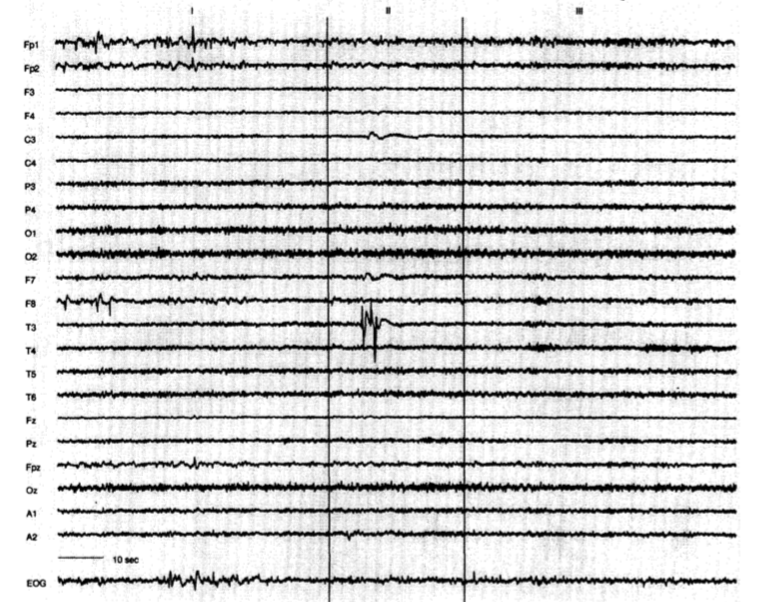
\includegraphics[scale=0.45]{imagenes/EEGData}
	\caption{EEG: Estudio de eliminación de artifacts oculares a través de ICA. Fuente \cite{EEG-Eye}} 
	\label{fig:EEGData}
\end{figure}

La propuesta recogida en \cite{EvolutionaryBigOpt} provee una forma de representar el problema de la decodificación de un QEEG, de forma que cualquier técnica, método o algoritmo preparado para el procesamiento de grandes cantidades de datos y la optimización global de miles de variables, pueda ser sometido a pruebas exhaustivas frente a este problema real, y finalmente sugerir, si cabe, un posible candidato que sustituya al actual método de decodificación, descrito en el párrafo anterior, con el último fin de dar un salto importante en el diseño de sistemas BCIs para la mejora de la calidad de vida de todas aquellas personas que lo requieran.

Como el estudio se basa completamente en la clara definición del problema en cuestión, los siguientes párrafos contendrán toda la información referente a éste, desde la representación elegida, pasando por las bases de datos disponibles y llegando hasta la definición de la función objetivo que marcará el camino a seguir en este estudio. Como aclaración, se habla de QEEG como un tipo de EEG utilizado en algunos campos, aunque a efectos prácticos para entender y describir el problema, se les considera equivalentes.

\section{Representación del problema: EEG}

Para definir el problema de la optimización de un EEG se ha empleado una representación que divide al problema en 3 subproblemas con la misma naturaleza que el original, donde únicamente cambian la dimensión del mismo y la existencia de ruido en los datos. De esta forma, se ha generado una base de datos sintéticos (generados de forma artificial)\cite{ICA-Calibrate} que se reúnen en tres Datasets \textbf{A, B y C} tal y como se muestra en la siguiente tabla.

\begin{table}[H]
	\centering
	\resizebox{\textwidth}{!}{
		$\begin{tabular}{ *{5}{c}}
		\toprule
			\textbf{Dataset}& \textbf{Nº Fuentes} & \textbf{Nº Artifacts} & \textbf{Sin ruido} & \textbf{Con ruido} \\
			\midrule
			\textbf{A} & 4 & 2 & D4 & D4N\\ 
			\textbf{B} & 12 & 6 & D12 & D12N \\ 
			\textbf{C} & 19 & 6 & D19 & D19N \\ 
			\bottomrule
		\end{tabular}$
	}
		\caption{Grupos del problema del EEG.}
		\label{tabla:gruposEEG}
\end{table}

Cada dataset propone una dificultad distinta en términos del número de fuentes de señales reales y de ruido con una \textbf{varianza de 0.1}. Las fuentes de señales efectivas son la suma del \textbf{número de fuentes de datos reales} y el \textbf{número de artifacts}, donde estos últimos operan en altas frecuencias y amplitudes. 

Las señales de los artifacts \textbf{simulan impulsos electromagnéticos} que se generan de forma involuntaria con movimientos de cualquier parte de nuestro cuerpo durante el tiempo en el que se recogen los datos en el EEG, y al ser señales eléctricas, son captadas por éste mezclándose con las señales reales de nuestro cerebro y empañando el EGG. Cada señal se muestrea a una frecuencia de \textbf{256Hz,} y los artifacts son activados en intervalos que oscilan entre los últimos \textbf{250ms-500ms} de cada segundo (ver \cite{ICA-Calibrate}).

Para el \textbf{Dataset A}, las 6 señales totales se mezclan en \textbf{4 señales de datos}, $\vv{x_1}, \vv{x_2}, \vv{x_3}$ y $ \vv{x_4} $ compuestas según las siguientes ecuaciones, donde las señales 5 y 6 son artifacts.

\begin{equation}\label{eq:D4}
	\begin{gathered}
		\vv{x_1} = \vv{s_1} + 0.9\vv{s_5}\\
		\vv{x_2} = \vv{s_2} + 0.9\vv{s_6}\\
		\vv{x_3} = \vv{s_3} + \vv{s_5}\\
		\vv{x_4} = \vv{s_4} + \vv{s_6}\\
	\end{gathered}
\end{equation}

Para los \textbf{Datasets B y C}, las 6 señales de artifacts se disparan en posiciones determinadas de la cabeza de una persona, indicadas  en la figura \ref{fig:artifactsLocation}. De forma análoga, cada fuente de datos real de las 12 (Dataset B) o 19 (Dataset C) se mezcla con cada una de las $k$ fuentes de artifacts siguiendo la ecuación:

\begin{equation}\label{eq:D12-9}
	\begin{gathered}
	\vv{x_i} = \vv{s_i} + \sum_{k=1}^{N} w_{ik} s_k\\
	w_{ik} = exp (-r^2)
	\end{gathered}
\end{equation}

donde $w_{ik}$ representa el exponencial de la distancia Euclídea al cuadrado con signo negativo de la señal \textit{i-ésima} y el artifact \textit{k-ésimo}. Esta distancia se calcula teniendo en cuenta la posición donde se colocan los electrodos (fuentes de datos reales) y desde donde se disparan los artifacts en una cabeza de radio 0,5dm, tal y como se puede ver en la figura.

\begin{figure}[h]
	\centering
	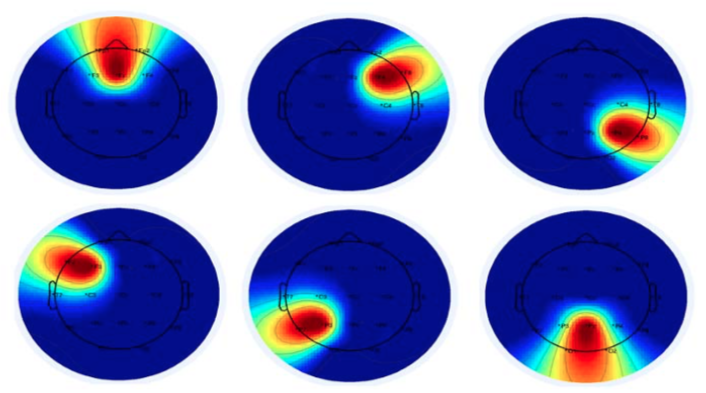
\includegraphics[scale=0.45]{imagenes/Artifacts}
	\caption{Disposición de los 6 artifacts y la contribución de cada uno en todos los electrodos. Fuente: \cite{EvolutionaryBigOpt}}
	\label{fig:artifactsLocation}
\end{figure}

En resumen, un total de \textbf{6 problemas distintos}, \textbf{D4, D4N, D12, D12N, D19 y D19N}, donde cada señal se muestrea a 256Hz, da lugar a \textbf{tres valores de dimensionalidad del problema} que repercuten directamente en la complejidad en cuanto a espacio de soluciones, donde cada dimensión se calcula como el \textbf{número de señales de entrada ($N$)} de cada problema multiplicada por la \textbf{frecuencia de muestreo (256Hz)}. Con esta definición se busca facilitar la representación interna de las soluciones como un único conjunto de variables a optimizar; así, el \textbf{Dataset A} tiene \textbf{1024} variables, el \textbf{Dataset B} cuenta con \textbf{3072} y el \textbf{Dataset C} concretamente dispone de \textbf{4864} variables.

Esta elección conceptual conforma la base de este estudio a nivel de representación de los datos, lo que permitirá evaluar el grado de desempeño de un algoritmo frente a la optimización de los datos simulados de un EEG, cuyos resultados son extrapolables a una aplicación médica real si se tiene en cuenta el proceso matemático y estadístico sobre el que se sustenta la decodificación de las señales medidas y que se describe a continuación.

\section{ICA: Independent Component Analysis}

Un Análisis de Componentes Independientes, \textbf{ICA} en inglés, es un método de procesamiento de señales utilizado principalmente para eliminar artifacts \cite{ICA-Calibrate}. Permite \textbf{separar en fuentes de datos independientes} aquellas fuentes que han sufrido transformaciones lineales y se encuentran mezcladas, a través de una maximización de la independencia estadística de las componentes resultantes\cite{ICA-EGG}.

A grandes rasgos un ICA consta de dos pasos, un primer paso donde se elimina toda la correlación de los datos, llamado \textit{data whitening}, y un segundo paso donde se aplica la matriz de rotación inversa a la transformación aplicada, con el fin de obtener los datos originales. La correlación de los datos se debe principalmente a que un electrodo localizado en una parte determinada de la cabeza, no sólo medirá los impulsos eléctricos de esa zona en particular, sino que también se verá afectado por las señales cercanas que estén siendo sensadas por otros electrodos. 

 Expresado de forma matemática, un ICA busca una \textbf{transformación lineal V} de los \textbf{datos D} de forma tal que $P = V\cdot D$ y que $Cov(P) = I$, siendo $Cov$ la matriz de covarianza e $I$ la matriz de identidad, lo que indica que las variables no tienen correlación alguna (paso 1, \textbf{data whitening}). Tras encontrar $V$, se procede a realizar la rotación de la matriz a través de la \textbf{minimización de la Gaussianidad} de la matriz en cuestión.
 
 Por tanto, el problema de la optimización del EEG se puede formular análogamente a la aplicación de un ICA de la siguiente manera:
 
 \begin{equation} \label{eq:problem1}
	 \begin{gathered}
		X = A\cdot S + N
	 \end{gathered}
 \end{equation}
 
 donde $X$ es la matriz combinada de señales (debido a la naturaleza de la medición), A es la matriz de combinación que representa la transformación lineal \textit{V} del ICA al combinarse las señales entre sí, \textit{N} es el ruido y \textit{S} las fuentes de datos originales; así al disponer de \textit{A} y unas fuentes estimadas $\hat{S}$, hay que encontrar \textit{W} tal que $\hat{S} = W\cdot X$. Finalmente se reconstruyen las señales limpias a través de las componentes útiles, tal que : $\hat{X} = W^{-1} \hat{S}$
 
 \section{Formulación del problema: enfoque uniobjetivo}
 
 La formulación original del problema sigue un enfoque multiobjetivo pero adoptar un \textbf{enfoque uniobjetivo} reduce la complejidad del problema sin incurrir en pérdida alguna de generalidad. Por tanto, se utilizará el enfoque multiobjetivo para formular el problema pero experimentalmente se generalizará a uno uniobjetivo.
 
 Sea \textit{X} (matriz combinada de señales) una matriz de dimensión $n\times m$ donde $n$ es el número de \textbf{series de tiempo interdependientes} y $m$ la \textbf{longitud} de cada serie. Sea a su vez \textit{S} (matriz de fuentes reales) una matriz $n\times m$ con $n$ series de tiempo \textbf{independientes} de longitud $m$ y \textit{A} una \textbf{matriz de transformación lineal} $n\times n$. Se sabe que:
 
  \begin{equation}
	 \begin{gathered}
	 	X = A\times S
	 \end{gathered}
 \end{equation}
 
 Por tanto el problema consiste en descomponer S en $S_1$ y $S_2$ tal que $S = S_1 +S_2$ y que además $X = A\times S_1 + A\times S_2$. Y sea $C$ la matriz de \textbf{coeficientes de correlación de Pearson} entre $X$ y $A\times S_1$ definida como:
 
 \begin{equation} \label{eq:covar}
	 \begin{gathered}
	 	C = \frac{covar(X,AS_1)}{\sigma(X)\cdot \sigma (A\cdot S_1)}
	 \end{gathered}
 \end{equation}
 
 donde $covar( )$ representa la matriz de covarianzas y $\sigma$ la varianza.
 El objetivo consiste en \textbf{maximizar los elementos diagonales de C} a la vez que se minimizan los elementos de fuera de la diagonal, y conseguir que la \textbf{distancia entre $S$ y $S_1$} sea la mínima posible, lo que a su vez maximice la similitud entre estas \cite{EvolutionaryBigOpt}. Para ello, se debe encontrar una matriz $S_1$ que minimice el valor de las siguientes funciones:
 
  \begin{equation} \label{eq:function1}
	 \begin{gathered}
	 	Minimize \ f_1 = \frac{1}{N^2 -N} \sum_{i}^{} \sum_{j \neq i}^{} C_{ij}^2 + \frac{1}{N} \sum_{i}^{} (1-C_{ii})^2
	 \end{gathered}
 \end{equation}
 
  \begin{equation} \label{eq:function2}
	 \begin{gathered}
	 	Minimize \ f_2 = \frac{1}{N \times M} \sum_{i}^{} \sum_{j}^{} (S_{ij} - S_{1ij})^2
	 \end{gathered}
 \end{equation}
 
 donde se busca \textbf{eliminar la mayor cantidad de artifacts posibles} a la vez que se \textbf{minimiza la pérdida de información real}. A través de estas dos funciones se propone el  \textbf{enfoque uniobjetivo} donde la función objetivo a optimizar es la siguiente:
 
 \begin{equation} \label{eq:FObj}
	 \begin{gathered}
	 	f = Minimize(f_1 + f_2)
	 \end{gathered}
 \end{equation}
 
 Queda definida por tanto la base sobre la que se construye este estudio, donde la función objetivo juega un papel principal en cuanto al problema de la optimización de los datos de un EEG. En el siguiente capítulo será revisada la literatura del problema en cuestión, además del conjunto de problemas más utilizados actualmente para la evaluación de los algoritmos, los denominados benchmarks, y por último los principales algoritmos y técnicas utilizados para problemas de tipo \textbf{LSGO}.
\chapter{Revisión de la literatura}\label{EstadoArte}

En este capítulo se revisa el estado actual de la literatura en cuanto a problemas de Big Optimization se refiere, en concreto los \textbf{benchmarks} más utilizados en esta rama. Una revisión del \textbf{estado del arte actual del problema del EEG} se llevará a cabo de forma análoga, prestando especial atención a las dos vertientes sobre las que se basa este estudio: las \textbf{técnicas previamente aplicadas} para resolver el problema del EEG y el estado del arte actual en cuanto a \textbf{algoritmos de optimización de miles de variables}, donde intervienen técnicas de distinta naturaleza, con el objetivo final de establecer el símil sobre el que se basa el desarrollo de este Trabajo Fin de Grado. 

\section{Estado del arte: CEC y Benchmarks}

Los problemas de optimización  han estado presentes desde los inicios de la computación evolutiva y una vertiente de estos, los \textbf{problemas de optimización de miles de variables (LSGO)}, se encuentra actualmente en auge dada la necesidad de resolución de problemas del mundo real donde la formulación de estos incurre en una representación con miles de variables que precisan de una optimización efectiva y eficiente.

\textbf{IEEE}, la organización profesional para el avance tecnológico más grande del mundo, ha sido desde 1999 la encargada de organizar el \textbf{Congress on Evolutionary Computation}, uno de las mayores y más importantes convenciones de computación evolutiva a nivel mundial \cite{IEEECEC}; en ella se exponen numerosas técnicas para resolver b que son evaluadas a través de distintas competiciones, y que cuya dimensionalidad no supone impedimento alguno a la hora de ser resueltos.

Sin embargo, no es hasta el año 2008 cuando se propone la primera \textbf{Special Session \& Competition on Large-Scale Global Optimization}\cite{CEC-LSGO}, con el objetivo de establecer una base sobre la que evaluar las distintas propuestas, algoritmos o técnicas destinadas a resolver\textbf{ problemas de optimización de alta dimensionalidad}, donde las técnicas disponibles en ese momento sufrían una considerable reducción de su rendimiento conforme aumentaba el tamaño del espacio de soluciones.

A partir de este momento entran en escena un \textbf{conjunto de problemas de optimización representados por funciones acotadas} que, a diferencia de años anteriores, contenía un elevado número de variables a optimizar. Este conjunto de funciones se agrupa dentro de lo que se denomina un \textbf{benchmark} o \textbf{test suite} que sirve para evaluar el desempeño de las técnicas de tipo LSGO.

Tras la evolución de los benchmarks a lo largo de la última década, se han añadido diferentes tipos de funciones que pretenden \textbf{estimar la calidad de las soluciones} de las técnicas más avanzadas cuando se enfrentan a distintos tipos de problemas, donde la \textbf{interacción de las variables} juega un papel fundamental a la hora de llevar a cabo una optimización efectiva, dado que ésta determina el \textbf{potencial o la capacidad} que tiene una variable para  \textbf{influir en el efecto de otra u otras variables} y por tanto ser determinante en la calidad de la solución obtenida.

Atendiendo a esta definición\cite{ELSGOI}, las funciones benchmark se agrupan formando distintas clases según el grado de interacción; así tenemos, principalmente, grupos de funciones \textbf{separables}, \textbf{parcialmente separables}, funciones con \textbf{subcomponentes solapadas} y funciones \textbf{completamente no separables}. La interacción de variables y sus grupos serán descritas en profundidad en el capítulo 4.

Los benchmarks propuestos para las distintas competiciones contienen habitualmente \textbf{entre 15 y 20 funciones} de distinto tipo como las funciones \textbf{Shifted Elliptic, Shifted Sphere, Rastrigin, Schwefel, Rosenbrock}, funciones híbridas variadas y otros tipos de problemas de elevada complejidad\cite{ComprehensiveComparison}. La dimensionalidad de estos problemas ronda las 1000 variables, por lo que supone un punto de partida robusto en cuanto a evaluación de las capacidades  de un algoritmo se refiere.

Actualmente, los benchmarks que sirven como principal referencia para los algoritmos dedicados a Big Optimization son los propuestos en las competiciones del \textbf{CEC 2010} y, mayoritariamente, los del \textbf{CEC 2013}\cite{CEC2013}, utilizados en la más reciente competición del WCCI 2018\cite{WCCI-SHADEILS}. Durante los siguientes apartados de esta revisión, se examinará el estado actual del problema del EEG así como de los algoritmos \textit{state-of-the-art} que han sido evaluados con respecto a los benchmarks descritos con anterioridad.


\section{Estado del arte: \textit{EEG Problem} y propuestas de solución}

En el año 2015, durante el IEEE Congress on Evolutionary Computation llevado a cabo en Sendai, Japón\cite{IEEE-CEC2015}, se presenta la  \textbf{Optimization of Big Data 2015 Competition}\cite{CompetitionBigOpt} donde, a diferencia de años anteriores, no se propone un conjunto de funciones benchmark de alta dimensionalidad sino un problema completamente distinto, el de la optimización de los datos de un electroencefalograma, que ha sido descrito en el capítulo anterior.

No se conocen con exactitud todas las técnicas propuestas para esta competición, pero tras ésta los organizadores publican el artículo \textit{Evolutionary Big Optimization (Big Opt) of Signals}\cite{EvolutionaryBigOpt}, en el que se recogen los resultados obtenidos al aplicar el problema sobre dos \textit{state-of-the-art} \textbf{MOEAs}, algoritmos evolutivos multiobjetivo: MOEA/D y NSGA-II.

\textbf{MOEA/D}\cite{MOEA/D} emplea la estrategia de descomposición para hacer frente a los problemas multiobjetivo: descompone el problema MO en un subconjunto de problemas y los optimiza de forma separada utilizando únicamente la información de los subproblemas vecinos, reduciendo considerablemente la complejidad del problema en cada generación si lo comparamos con el algoritmo \textbf{Nondominated Sorting GA II} (NSGA-II)\cite{NSGA-II}, que posee una complejidad de orden $O(MN^2)$ siendo \textit{M} la cantidad de objetivos y \textit{N} el tamaño de la población; el algoritmo crea una \textit{mating pool} donde la población de padres y offsprings se combinan, eligiendo posteriomente el mejor de estos, dando solución a los impedimentos típicos de los algoritmos MO que utilizan clasificación no-dominada.

En el artículo mencionado anteriormente, se propone el enfoque \textbf{multiobjetivo}, optimizando por separado ambas funciones \ref{eq:function1} y \ref{eq:function2}. Se elige optimizar dos representaciones distintas, frente al \textbf{dominio del tiempo} y al \textbf{de la frecuencia}; este último para intentar superar los inconvenientes derivados de la dimensionalidad del problema.

Los resultados muestran un mejor desempeño de \textbf{MOEA/D} frente a NSGA-II en la representación frente al dominio de la frecuencia, dado que esta, a través de una \textbf{Fast Fourier Transform} aplicada sobre los componentes principales, es capaz de reducir \textbf{hasta la mitad la dimensionalidad} del problema (con una frecuencia de 1Hz). La r\textbf{educción de la dimensionalidad} y los\textbf{ buenos resultados} conseguidos son las principales bazas a tener en cuenta de cara a una aplicación real donde los datos de un EEG sean procesados y posteriormente ``blanqueados" por algoritmos evolutivos multiobjetivo.

\subsection{MAGA-BigOpt: Algoritmo Genético Multi-Agente para optimización uniobjetivo}

\textbf{MAGA-BigOpt}, \textbf{\textit{A Multi-Agent Genetic Algorithm for Big Optimization Problems}}\cite{MAGA-BigOpt}, es la principal propuesta de solución para el problema del EEG formulado en la Optimization of Big Data 2015 Competition, con enfoque uniobjetivo. Esta técnica, basada en un framework MAGA, ``r\textit{eestructura los operadores de competición y autoaprendizaje, que finalmente combina con operadores de cruce y mutación para \textbf{simular la cooperación, competición y comportamientos de aprendizaje de los agentes}}".

MAGA, en primera instancia propuesto para optimización numérica global a gran escala en\cite{MAGA} , evolucionó para resolver el problema en cuestión, EEG, con 4 operadores genéticos donde un operador de autoaprendizaje con subgradiente es su principal activo, obteniendo resultados que superan con creces los propuestos como base en la competición mencionada.

Este algoritmo se basa en la idea de \textbf{agente}, que no es más que una solución candidata, y la \textbf{energía de un agente} computada como el valor negativo de la función $f$ definida en la ecuacion \ref{eq:FObj}. Los agentes se encuentran en un entorno similar a una rejilla $L$, que se llama la rejilla de agente, con tamaño $L_{size}\times L_{size}$. La representación vectorial de un agente (solución) permite situarlo en una posición $L_{i,j}$ donde tendrá 4 vecinos espacial subyacentes: arriba, abajo, izquierda o derecha según donde se encuentre en la rejilla. 

El objetivo consiste por tanto en maximizar la energía de los agentes a través de los operadores evolutivos propuestos, donde los procesos de competición y cooperación son llevados a cabo por los \textbf{operadores de competición y cruce de vecinos} respectivamente, mientras que el uso del conocimiento del contexto se basa en los operadores de cruce y autoaprendizaje. La descripción completa de cada uno de los operadores y su aplicación se puede consultar en \cite{MAGA-BigOpt}.

Atendiendo a los resultados obtenidos tras aplicar MAGA-BigOpt sobre el problema del EEG, tanto en problemas con ruido como sin este, se observan valores superiores a los propuestos como base en la competición, alcanzando valores muy cercanos a cero y con una varianza prácticamente despreciable, hecho que junto a la potencia de los operadores propuestos, reafirma la candidatura de esta técnica a ser considerada como estado del arte actual en cuanto a la resolución del problema del EEG. Por tanto, \textbf{servirá como punto de referencia} en este estudio tanto a niveles de calidad de la solución como a restricciones de tiempo, al elegir utilizar el mismo enfoque, uniobjetivo, por el que se ha optado en este trabajo.

\section{Estado del arte: Algoritmos LSGO} \label{cap:revisionLSGO}

Los computación evolutiva a través de algoritmos dedicados a la resolución de \textbf{problemas de optimización global continua con miles de variables} es un campo que, como anteriormente ha sido mencionado, ha sufrido una creciente y rápida evolución en cuanto al número de propuestas debido a la necesidad de plantear soluciones efectivas y sobre todo eficientes a una gran cantidad de problemas reales que pueden ser representados mediante un problema de Big Optimization.

La \textit{Special Session and Competition on Large-Scale Global Optimization} del WCCI 2018\cite{WCCI-SHADEILS} indica que no es hasta el año 2015 cuando se experimenta un cambio significativo entre la cantidad de artículos publicados en esta materia y los propuestos únicamente para conferencias; así lo refleja el gráfico de la figura \ref{fig:LSGO-Evolution}, donde los resultados que arroja la búsqueda del término ``\textit{Large Scale Global Optimization}"\ en la base de datos Scopus\cite{SCOPUS}, sitio desde el que se han obtenido la gran mayoría de referencias bibliográficas que se encuentran en este trabajo.

Un estudio publicado en 2014 bajo el nombre de \textbf{\textit{A comprehensive comparison of large scale global optimizers}}\cite{ComprehensiveComparison} recoge la comparativa entre las \textbf{tres mejores propuestas} de las sesiones del CEC 2010, CEC 2012, CEC 2013 y SOCO 2011 con el objetivo de \textbf{analizar el desempeño global} de aquellas técnicas cuando son evaluadas con respecto a\textbf{ tres distintos benchmarks} con distintos tipos de funciones, para determinar no solo la efectividad y eficiencia de forma individual sino también de manera global.

\begin{figure}[h]
	\centering
	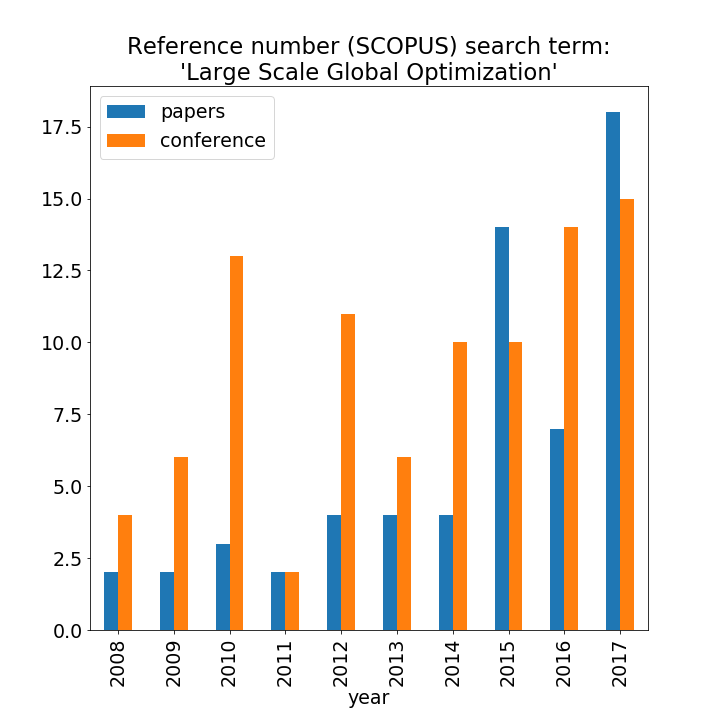
\includegraphics[scale=0.5]{imagenes/LSGO-Evolution}
	\caption{Evolución de las referencias de propuestas de algoritmos LSGO. Fuente: \cite{WCCI-SHADEILS}}
	\label{fig:LSGO-Evolution}
\end{figure}

\subsection{Estado del arte: SOCO 2011 Special Issue}
La \textit{SOCO 2011 Special Issue} cuenta con fuertes propuestas como lo son \textbf{\textit{A MOS-based dynamic memetic differential evolution algorithm for continuous optimization: a scalability test}}\cite{MOS2010}, o MOS-SOCO2011, un algoritmo que basándose en la utilización del framework MOS (Multiple Offspring Sampling), es capaz de \textbf{combinar distintas estrategias de búsqueda} sin tener ninguna fuga; se combinan en este caso un algoritmo de \textbf{evolución diferencial (DE)} y la primera de las tres búsquedas locales del algoritmo MTS\cite{MTS-LSGO}, la \textbf{MTS-LS1}.

Ajustando la participación de cada técnica en base a una función de participación híbrida que favorece la utilización de aquella técnica que ha desempeñado mejor en base a dos medidas distintas, el algoritmo es capaz de obtener resultados muy competitivos, logrando vencer a los demás contrincantes en la competición.
 
Teniendo en cuenta que la evolución diferencial (DE)\cite{DE} es considerada actualmente una de las técnicas más potentes en cuanto a optimización continua, otra propuesta interesante a tener en cuenta de esta misma competición es \textbf{\textit{Scalability of generalized adaptive differential evolution for large-scale continuous optimization (GaDE)}}\cite{GaDE}, una generalización del DE adaptativo en el que a través de una distribución de probabilidad es capaz de \textbf{estimar el valor de cada uno de los parámetros para cada individuo} de la población. Esto se consigue haciendo que la distribución de probabilidad oscile en cada generación en función de las mejoras en fitness de cada individuo, confiriéndole una gran potencia al algoritmo a la vez que lo situa como posible técnica candidata a representar una futura solución.

\subsection{Estado del arte: CEC 2013 y CEC 2015}

Aunque las propuestas del CEC 2012 no llamen significativamente la atención, por tratarse de técnicas parecidas a las del SOCO 2011 pero con ligeros cambios, en las del \textbf{CEC 2013} se encuentran candidatos muy interesantes como lo son el \textit{Large Scale Global Optimization: experimental results with MOS-based hybrid algorithms}\cite{MOS2013}, técnica que combina un algoritmo genético con dos búsquedas locales muy conocidas y potentes, otra vez, a través del framework MOS: la del algoritmo \textbf{Solis Wets}\cite{SolisWets} y la \textbf{MTS-LS1 Reduced}, una modificación de la MTS-LS1\cite{MTS-LSGO} desarrollada exclusivamente para esta competición donde son optimizadas aquellas variables que contribuyen en mayor medida a una mejora en la calidad de las soluciones.

En esta misma sesión disponemos de una entrada que llama la atención en particular. A pesar de quedar en tercer lugar dentro de esta competición, \textit{Scaling up Covariance Matrix Adaptation Evolution Strategy using cooperative coevolution}\cite{CC-CMAES} o (CC-CMA-ES) es interesante debido a la formulación de la propuesta: dividir el problema en subproblemas más pequeños que serán optimizados utilizando la técnica evolutiva de adaptación por matrices de covarianza CMA-ES. Considerando la dimensionalidad del problema presentado en este trabajo, estrategias de \textbf{descomposición o subdivisión en problemas más pequeños} se postulan como plausibles alternativas a tener en cuenta de cara al estudio.

Durante el \textbf{CEC2015} tuvo lugar una competición de Large-Scale Global Optimization, cuyos resultados se encuentran disponibles en \cite{CEC15-Res-LSGO} y donde algunas técnicas como CC-CMA-ES o MOS  repiten aparición, siendo finalmente \textbf{MOS} el algoritmo que obtiene mejores resultados de forma global, hito que también logró durante el CEC 2013. De esta forma, se refuerza la concepción que se tiene de estos algoritmos como fuertes candidatos a proponer soluciones efectivas a los problemas de optimización de alta dimensionalidad.

\subsection{Estado del arte: WCCI 2018 Competition on LSGO}

Finalmente, observando los resultados de la más reciente competición en materia de LSGO,la \textbf{Special Session and Competition on Large-Scale Global Optimization, WCCI 2018} se proponen dos algoritmos que, dada las características y los resultados que obtienen, llaman la atención de manera significativa. En el momento del desarrollo de este trabajo, los papers referentes a ambas propuestas, \textit{SHADE with Iterative Local Search for Large-Scale Global Optimization}\cite{SHADEILS} y \textit{LSHADE-SPA Memetic Framework for Solving Large Scale Problems}\cite{ML-SHADE-SPA}, se encuentran bajo publicación, pero los resultados y toda la información referente a estos se encuentra disponible en \cite{WCCI-SHADEILS}. 

El primero, SHADEILS, es un algoritmo con una construcción muy similar a una propuesta anterior denominada IHDELS\cite{IHDELS} pero con tres principales diferencias que lo sitúan por encima de su antecesor: mecanismo de \textbf{elección de LS mejorada}, mecanismo de \textbf{reinicio de la población} y el uso de \textbf{SHADE}\cite{SHADE} en vez de SaDE\cite{SaDE}. 

Se elige una LS de entre  MTS-LS1\cite{MTS-LSGO} y L-BFGS-S\cite{LBFGSB}, siendo ambas complementarias: mientras que la primera es rápida pero sensible a rotaciones del sistema de coordenadas, la segunda es mas lenta pero insensible a este tipo de rotaciones. Además, al utilizar SHADE, autoajusta sus parámetros basado en la \textit{historia} y manteniendo la población entre iteraciones, consigue intensificar el proceso de exploración. 

Por otra parte el segundo, ML-SHADE-SPA, es un framework que utiliza \textbf{tres algoritmos basados en poblaciones} para el proceso de \textbf{exploración}, LSHADE-SPA, EADE y ANDE, mientras que el proceso de \textbf{explotación} es llevado a cabo por una \textbf{versión modificada del algoritmo MTS}. Introduce además la idea de \textbf{divide y vencerás}: se mezclan de forma aleatoria las dimensiones y se resuelven de forma separada. Este proceso es completamente independiente de cualquier tipo de información, esto es, las particiones se realizan sin tener en cuenta ninguna suposición acerca de la estructura del problema, añadiendo robustez al algoritmo y confiriéndole un grado de generalización que le permite hacer frente a disintos problemas siguiendo el mismo enfoque.

Cabe destacar que estos dos algoritmos han logrado desbancar al, hasta este año, algoritmo considerado como estado del arte, el mencionado anteriormente \textbf{MOS}, por lo que son los más fuertes candidatos a tener en cuenta en este estudio. Para finalizar, se revisarán las propuestas de algoritmos de descomposición de variables y las posibles ventajas que puede aportar a favor de la resolución del problema tratado en este trabajo.

\section{Estado del arte: algoritmos de descomposición de variables}

La interacción de las variables del problema que requiere de optimización juega un papel fundamental en el proceso de obtención de soluciones óptimas. Es por ello que surgen técnicas de \textbf{descomposición} y \textbf{co-evolución cooperativa} como alternativas para hacer frente al problema inherente de la interacción. De forma análoga, la descomposición del problema en \textbf{subproblemas más pequeños} favore la reducción de dimensionalidad global del problema y por consiguiente disminuye la complejidad del espacio de soluciones.

\textbf{Cooperative Co-Evolution (CC)}\cite{CCoevo} es el framework por excelencia para guiar el proceso de optimización una vez creadas las descomposiciones, el cual requiere de un \textbf{agente} (un algoritmo evolutivo, principalmente) para coordinar como se aplica este agente a las distintas componentes de descomposición; no obstante, la \textbf{descomposición del problema} sigue siendo un impedimento considerable. La descomposición óptima es aquella que \textbf{minimiza la interacción} entre las componentes descompuestas y aquí entran en juego técnicas de agrupación como \textbf{Random Grouping o Delta Grouping}, donde es \textbf{Differential Grouping (DG)-2014} \cite{DG} la propuesta que ha alcanzado mejores cotas de éxito, utilizando conceptos como \textbf{función aditivamente separable} y \textbf{forward difference} para detectar las interacciones.

Existen una familia completa de este tipo de propuestas, donde están incluidas  \textbf{Global Differential Grouping}\cite{GDG}, \textbf{eXtended Differential Grouping}\cite{XDG} o la más reciente incorporación \textbf{Differential Grouping 2} (DG2)\cite{DG2}. Cada una de estas propuestas aborda el problema de la descomposición de variables siguiendo el mismo precepto pero centrándose en características particulares, como la detección directa o indirecta de interacciones. 

Esta grupo de técnicas conforman un bloque con fuerte base matemática que ha mostado resultados muy competitivos, sobretodo cuando las componentes individuales son optimizadas de forma cooperativa con el \textbf{framework CC} a través agentes robustos tales como \textbf{MOS, CMA-ES o MA-SW-Chains}, por lo que dada la dimensionalidad del problema y los beneficios que implica el uso de este tipo de técnicas, si se satisfacen las condiciones necesarias, aspiran a formar parte de una solución efectiva para el problema del EEG.


\section{Crítica al estado del arte}

Tras analizar los puntos fuertes de las actuales técnicas de resolución de problemas en el ámbito de Big Optimization, el siguiente punto a revisar tiene que ver con la \textbf{identificación de las principales deficiencias} de las técnicas a nivel estructural y de eficiencia y eficacia, con el objetivo de justificar el desarrollo de este trabajo.

El primer punto a considerar es la \textbf{elevada complejidad estructural} de muchas de las técnicas propuestas: a pesar de responder de forma satisfactoria a los benchmarks, su estructura interna muchas veces añade complejidad al problema, ya sea por disponer de \textbf{técnicas de exploración o explotación costosas} a nivel computacional o por perjudicar el \textbf{balance exploración-explotación}, lo que finalmente repercute en la calidad de las soluciones. Técnicas como las basadas en el framework MOS o las de optimización multiobjetivo son sumamente complejas a nivel tanto \textbf{conceptual} como \textbf{estructural}.

La siguiente cuestión esta directamente relacionada con la anterior y es el \textbf{excesivo coste computacional en tiempo} que es necesario para obtener una solución relativamente sensata para este tipo de problemas. No es especialmente preocupante con dimensiones de, por ejemplo, 1000 variables, pero para el problema del EEG donde se manejan hasta 4864 variables se hace completamente inviable el proponer una solución para un problema médico del mundo real. 

Con la formulación uniobjetivo, donde se \textbf{minimiza} a la vez la \textbf{pérdida de información} y la \textbf{prevalecencia de artifacts} tras el proceso de limpieza del EEG, algoritmos como MAGA tardan alrededor de dos horas para el problema sin ruido, siendo el tiempo casi una hora superior cuando se trata de problemas con ruido. Para la formulación multiobjetivo, la representación frente al dominio del tiempo no es siquiera planteada con algoritmos como MOEA/D o NSGA-II, que a pesar de proveer soluciones razonables, siguen empleando demasiado tiempo de computación.

Estos dos preceptos reafirman la \textbf{imposibilidad} de tratar el problema con este tipo de algoritmos, por lo que son necesarias técnicas no más potentes pero si \textbf{más rápidas y con menor sensibilidad al ruido}. De otra forma, una técnica propuesta no tendrá utilidad real futura si se busca aplicarla a un ámbito de tiempo real, como se comentaba en el anterior capítulo, lo que repercutiría de forma negativa en el intento de mejora de la calidad de vida de muchas personas.

La familia de técnicas de DG por su parte son especialmente sensibles a clases de funciones cuyas \textbf{componentes descompuestas presentan solapamiento} entre sí, efecto cuya probabilidad de existencia aumenta cuanto mayor es el número de variables. Adicionalmente, son muy \textbf{sensibles} a los valores del \textbf{umbral de detección de interacción} que es definido previamente, por lo que su desempeño en cuanto a calidad de soluciones se podría ver truncado frente a problemas con ruido y su eficiencia verse perjudicada cuando se requiera comprobar todas los pares de variables para detectar las interacciones.

Por último mencionar que la gran mayoria de los algoritmos propuestos, han seguido una \textbf{lenta evolución} en cuanto a publicaciones efectivas tal y como se puede ver en la figura \ref{fig:LSGO-Evolution}; hasta hace apenas tres años, la gran mayoría de propuestas se remitían únicamente a los congresos, conferencias y competiciones, siendo estudiadas y evaluadas sobre benchmarks poco representativos del panorama del LSGO actual. En resumen, actualmente no se dispone de \textbf{suficientes propuestas potentes} como para hacer frente a problemas de optimización del mundo real con total efectividad. 

\section{Propuesta}\label{Propuesta}

El estado del arte actual abre una posibilidad de estudio sobre un problema real de cara a paliar los inconvenientes reflejados anteriormente, tomando como punto de referencia el problema del EEG. El estudio se centrará principalmente en llevar a cabo una \textbf{adaptación híbrida de los algoritmos} considerados \textit{state-of-the-art} de forma que sean capaces de procesar la función objetivo que representa el problema del EEG y de proveer resultados que solucionarán, en caso tal, las deficiencias anteriormente expuestas.

Mediante un estudio experimental lo suficientemente completo, se pretende dar respuesta y una posibile solución a los tres inconvenientes destacados en el apartado anterior. Encontrar técnicas potentes en las que \textbf{prime una calidad de soluciones alta}, mejor o igual a la propuesta por el algoritmo \textbf{MAGA} (dado el enfoque uniobjetivo elegido), que será el algoritmo de referencia con el que comparar, utilizando para ello, las técnicas más adecuadas según los criterios que mencionabamos anteriormente, donde cada elección estará guiada por la posibilidad de hacer frente a estos inconvenientes.

La técnica elegida para este fin también deberá dar solución a los dos primeros problemas: la \textbf{complejidad conceptual-estructural debe ser la mínima posible} y los \textbf{tiempos de respuesta efectivos deben ser razonablemente adecuados} a la naturaleza del problema cuando se aplica a un entorno de tiempo real. De esta forma, aunque un algoritmo sea considerado estado del arte en la actual literatura, no se tendría en consideración alguna de cara a la resolución de un problema de optimización real de miles de variables, siendo únicamente válido en términos de evaluaciones frente a benchmarks.

Aquel algoritmo que muestre el desempeño más adecuado de acuerdo a las anteriores primitivas, independientemente de si ha conseguido solventar de forma total o parcial los tres escenarios anteriores, se someterá a estudio bajo un \textbf{algoritmo de descomposición de variables}, para comprobar si la \textbf{optimización por separado de grupos de variables} implica realmente una \textbf{reducción de la dimensionalidad} a nivel individual del problema

La implementación de este proceso está sujeta al tipo de función con la que se enfrenta el algoritmo y la factibilidad de la aplicación de técnicas de cooperación co-evolutiva depende directamente de los factores derivados de la naturaleza de la función, principalmente su dimensionalidad, lo que influirá de forma determinante en el \textbf{tiempo de respuesta}; estas son las condiciones que se deben cumplir para poder llevar a cabo una hibridación que tenga la capacidad de obtener mejores resultados sin dejar de ser útil a efectos prácticos.

Posteriormente, se emitirá un juicio en cuanto a si se consigue mejorar los resultados que proporciona el algoritmo base elegido. En caso favorable, se propondrá una solución lo suficientemente respaldada de cara a ser implementada en sistemas BCIs donde se pueda estudiar de forma mucho mas eficiente y efectiva un EEG cuantitativo, incluso en entornos donde se requiera respuesta en tiempo real. 
\chapter{Análisis de las Propuestas: Algoritmos LSGO}\label{cap:Analisis}

La finalidad de esta sección consiste en dar respuesta a las tareas \ref{tarea3} y \ref{tarea4} planteadas en el capítulo \ref{cap:Requisitos} donde se propone, principalmente, \textbf{analizar de forma exhaustiva los distintos algoritmos} seleccionados como fuente de estudio en este trabajo. 

El análisis está organizado de forma que se expongan todos los aspectos relevantes del algoritmo en cuestión tales como la \textbf{representación matemática} de su composición, \textbf{estructura interna} de la técnica, \textbf{elementos esenciales}, características particulares de la \textbf{implementación}, así como de la motivación para su \textbf{elección}, que estará basada esencialmente en los elementos anteriores, y en general, cualquier detalle significativo que aporte información relevante para este trabajo.

Al término de este capítulo se habrán completado las tareas necesarias para iniciar el proceso de \textbf{adaptación de las técnicas} al problema del EEG, donde se repasarán \textbf{aspectos fundamentales de la propuesta de problema} relacionados con la representación e implementación en código fuente y que sentará las bases del  \textbf{proceso experimental} que finalmente conduzca a la generación de resultados, que serán en última instancia evaluados e interpretados y conformarán la base de las conclusiones pertinentes.

\section{Multiple Offspring Sampling (2011)}

La primera propuesta elegida para este estudio es la conocida como \textbf{MOS2010}, dado que fue formulada en ese año y utilizada en la posterior competición del CEC 2011\cite{ComprehensiveComparison}. La publicación llega bajo el nombre de \textbf{\textit{A MOS-based dynamic memetic differential evolution algorithm for continuous optimization: a scalability test}} \cite{MOS2010}.

A grandes rasgos, en la publicación se propone un innovador \textbf{algoritmo memético híbrido} que a través del framework MOS (Multiple Offspring Sampling)\cite{MOS-Framework} \textbf{combina distintas estrategias de búsqueda} con el objetivo de alcanzar un balance exploración-explotación óptimo, en concreto, dos técnicas heurísticas que aplicadas por separado han mostrado resultados altamente competitivos.

La elección de este algoritmo como primer candidato está motivada por las siguientes razones: es la \textbf{primera formulación de MOS} que se propone para la conferencia del \textbf{SOCO 2011}, donde su diseño totalmente innovador se rige por las exigencias típicas de problemas de Big Optimization. Además, fue la técnica ganadora de esta edición, superando a otras que a pesar de utilizar algoritmos de evolución diferencial (DE), no consiguieron superar el rendimiento de MOS, y dónde algunas de estas técnicas eran estructuralmente más complejas.

La incorporación de la búsqueda local \textbf{MTS-LS1} de \cite{MTS-LSGO} ha sido otro de los principales motivos de su elección; tras la primera \textit{Special Session on Large-Scale Global Optimization} de 2008, el algoritmo MTS fue el que obtuvo mejores resultados para problemas de alta dimensionalidad, por lo que su uso en este algoritmo híbrido presenta una ventaja sustancial de partida frente a otras técnicas dada las capacidades de exploración que MTS añade durante el proceso de explotación.

Finalmente, MOS2011 \textbf{sentó la base del algoritmo} que durante los últimos 5 años ha sido considerado como \textit{state-of-the-art} en problemas LSGO, donde la formulación matemática subyacente relacionada con la \textbf{calidad de las soluciones} y la \textbf{participación} de cada técnica en el proceso tienen un rol fundamental, dado que estas contemplan dos tipos de mediciones que implican que cada técnica no solo debe mejorar sustancialmente las soluciones, sino además un buen porcentaje de éstas, lo que otorga más capacidad de respuesta ante el problema del estancamiento. Revisada la motivación de la elección, una descripción detallada de todo el algoritmo se expone a continuación.

El algoritmo enunciado propone dar solución al inconveniente que surge del aumento de la dimensionalidad sobre un problema, incluso cuando la naturaleza del mismo no cambia. Es aquí donde entra en juego el framework MOS, que permite combinar dos potentes técnicas: un algoritmo de \textbf{evolución diferencial (DE)} y la primera de las \textbf{búsquedas locales} (LS) del algoritmo MTS, la conocida como \textbf{MTS-LS1}\cite{MTS-LSGO}.

Este framework permite combinar distintas metaheurísticas siguiendo distintos tipos de enfoque, donde ha sido el \textbf{HRH} (High-level Relay Hybrid) el que se ha elegido; mediante esta perspectiva en particular, se \textbf{ajusta de forma dinámica} el número de \textbf{evaluaciones de la función objetivo} que cada algoritmo puede realizar. Para comprender la naturaleza de este enfoque es imprescindible conocer el origen de la terminología y de los demás enfoques.

En el artículo \textbf{\textit{A taxonomy of hybrid metaheuristics (2002)}	}\cite{TaxonomyEAs} se propone una taxonomía de los algoritmos híbridos, con el fin de establecer una terminología común a estos mecanismos, donde se combinan \textbf{esquemas jerárquicos}, para reducir la cantidad de clases, y \textbf{planos}, para cuando las clases que definen cada algoritmo se eligen de forma arbitraria. De esta taxonomía surgen 4 tipos de estrategias principales que detallamos a continuación:

\begin{enumerate}
	\item \textbf{LRH - Low-level Relay Hybrid}: una técnica metaheurística se incrusta en otra de \textbf{una sola solución}. Algoritmos de Simmulated Annealing (SA) combinados con LS son ejemplos de este enfoque.
	
	\item \textbf{LTH - Low-level Teamwork Hybrid}: la técnica es \textbf{incrustada en otra metaheuristica basada en poblaciones}. Un claro ejemplo de este tipo de enfoques es un algoritmo genético \textbf{GA} cuyo operador de mutación o cruce introduzca comportamientos que aumenten la capacidad de explotación del algoritmo.
	
	\item \textbf{HRH - High-level Relay Hybrid}: este enfoque ejecuta las metaheurísticas de \textbf{forma secuencial}, una a continuación de la otra. Es el enfoque elegido en esta propuesta, por lo que se requiere un mecanismo de control para organizar las técnicas y su ejecución.
	
	\item \textbf{HTH - High-level Teamwork Hybrid}: distintas técnicas son ejecutadas en paralelo, donde cada una se sirve de la información de las demás, cooperando en conjunto para encontrar soluciones óptimas. Aquí se pueden mencionar las técnicas basadas en CC (Cooperative Co-evolution).
\end{enumerate}

La técnica que se propone en esta publicación se basa en la hibridación de distintas técnicas, donde los algoritmos de evolución diferencial (DE) han sido los más utilizados a lo largo de los años. De forma complementaria, el algoritmo MTS\cite{MTS-LSGO} fue capaz de resolver problemas de hasta 1000 variables en el CEC 2008, valiéndose de \textbf{tres poderosas búsqueda locales}, razón por la cual se presenta como integrante de esta propuesta en particular. Así, el algoritmo DE dejaría lugar a que la LS encontrase regiones mas prometedoras a la vez que se reducen las evaluaciones a la función objetivo y por otra parte, la propia búsqueda local intentaría paliar los efectos del estancamiento en este tipo de algoritmos.

En esta propuesta en particular, el término \textbf{técnica de descendencia} hace referencia a \textbf{cualquier mecanismo para crear soluciones candidatas}, donde además son necesarios otros cuatro elementos: un modelo de algoritmo evolutivo en particular, una codificación de las soluciones, operadores específicos y parámetros necesarios. 

Esta característica implica que se pueden utilizar de \textbf{forma simultánea} varias técnicas para generar descendientes, lo que a su vez conlleva la existencia de un mecanismo que controle el uso de estas. El framework MOS propone dos grupos de funciones para solventar este inconveniente, lo que le permite \textbf{ajustar de forma dinámica el grado de participación de cada técnica} durante el proceso de búsqueda:

\begin{itemize}
	\item \textbf{Funciones de Calidad}: evalúan el fitness de los individuos en función de alguna característica deseable
	\item \textbf{Funciones de Participación}: asigna la cantidad de descendientes que genera cada técnica en función de la calidad de las soluciones.
\end{itemize}

El autor de la propuesta considera dos tipos de algoritmos según la taxonomía formulada en \cite{TaxonomyEAs}, estos son, HTH y HRH, sin embargo, se opta finalmente por el algoritmo de tipo \textbf{HRH}. En este tipo de algoritmos, las técnicas elegidas, en nuestro caso DE y MTS-LS1, son aplicadas en secuencia una a continuación de la otra, y cada una de cierta forma reutiliza la población resultante de la anterior. Este enfoque es más adecuado debido a que se utiliza en este caso una técnica no poblacional, como es la búsqueda local en cuestión.

El proceso de búsqueda se establece al principio de la ejecución, dividiendo el mismo en un \textbf{número fijo de pasos}. A cada paso se le asigna un número \textbf{fijo} de evaluaciones de la función objetivo, que son administradas de forma interna por cada técnica a través de la \textbf{función de participación} de la misma. De forma aclaratoria se expone el pseudocódigo de la propuesta HRH y se remite al lector a \cite{MOS2010} si se quiere profundizar en la propuesta HTH.

\begin{algorithm}[H]
	\begin{algorithmic}[1]
		\STATE Crear población de soluciones candidatas $P_0$
		\STATE Distribuir la participación uniformemente entre las $n$ tecnicas usadas $\rightarrow$ $\forall j \ \Pi_{0}^{(j)} = \frac{FE_{s_{0}}}{n}$. Cada tecnica produce un subconjunto de individuos de acuerdo con su participacion $ \Pi_{0}^{(j)}$
		\STATE Evaluar $P_0$
		\WHILE {no se supere el numero de pasos}
		\STATE Actualizar la Calidad de la técnica $T^{(j)}$ como la media de la calidad de los individuos que ha creado en el paso anterior
		\STATE Actualizar los ratios de participación en función de los valores de calidad del paso 5 $\rightarrow$ $\forall j \ \Pi_{i+1}^{(j)} = PF(Q_i^{(j)})$
		\STATE Actualizar el número de evaluaciones de la función objetivo de cada técnica $\rightarrow$ $\forall j \ FE_{s_i}^{(j)} = \Pi_{i+1}^{(j)} \cdot FE_{s_i}$		
		
		\FOR {cada tecnica $T^{ (j) }$}
			\WHILE{no se supere $FE_{s_i}^{ (j) }$ }
				\STATE Evolucionar
			\ENDWHILE
		\ENDFOR
		\ENDWHILE		
	\end{algorithmic}
	\caption{: HRH MOS } \label{Alg: MOS HRH}
\end{algorithm}

Como se puede observar, la participación de cada técnica depende de una función de calidad $Q$ que toma en consideración dos características: el \textbf{incremento medio del fitness} de los individuos tras la evaluación y el \textbf{número de veces} que se ha producido esta mejora. Se representa en la siguiente ecuación:

\begin{equation}\label{eq:QF_MOS}
	\begin{gathered}
		Q_i^{(j)} = 
						\begin{cases}
							\Sigma_{i-1}^{(j)} \ \textbf{if}  \ \forall k,l \in [1,n]: \Sigma_{i-1}^{(k)} > \Sigma_{i-1}^{(l)} \implies \Gamma_{i-1}^{(k)} > \Gamma_{i-1}^{(l)} \\ \\
							\Gamma_{i-1}^{(j)} \ \textbf{otherwise}
						\end{cases}
	\end{gathered}
\end{equation}

donde \\ \\
$Q_i^{(j)} \equiv$ Calidad de la técnica $T^{(j)}$ en el paso $i$\\
$\Sigma_i^{(j)} \equiv$ Incremento medio del fitness de $T^{(j)}$ en el paso $i$\\
$\Gamma_i^{(j)} \equiv$ Num. de mejoras de fitness de $T^{(j)}$ en el paso $i$	

En esta función de calidad $Q$ se utiliza $\Sigma_{i}^{(j)}$ si y sólo si hay consenso entre el incremento medio de fitness y el número de mejoras de una técnica a otra. En caso contrario se usa solo el número de incrementos del fitness. Esto es así debido a que una técnica que no este explorando el espacio de soluciones de forma adecuada, puede introducir grandes mejoras en el fitness, lo que puede no ser representativo. Estas acciones se penalizan en favor de comportamientos más adecuados, tales como mejoras relativamente pequeñas sobre buenos individuos de la población.

Una \textbf{función de participación dinámica} utiliza estos valores de $Q$ para ajustar el número de evaluaciones de la función objetivo asignado a cada técnica en cada paso. La función de participación $PF$ calcula, para cada paso del algoritmo, un \textbf{factor de compensación} $\Delta_i^{(j)}$ para cada técnica, lo que representa el decrecimiento de participación para cada técnica excepto para la mejor. Cada una aumentará su participación en proporción al cociente $\frac{\Sigma \Delta_{i}^{(j)}}{nº tecnicas}$. La $PF$ se describe en la siguiente ecuación:

\begin{equation}\label{eq:PF_MOS}
	\begin{gathered}
		PF_{dyn}(Q_i^{(j)} )= \begin{cases}
			\Pi_{i-1}^{(j)} + \eta \ \textbf{if} \ j \in best \\ \\
			\Pi_{i-1}^{(j)} - \Delta_i^{(j)} \ \textbf{otherwise}
		\end{cases}
	\end{gathered}
\end{equation}

$$
\eta = \frac{\Sigma_{k\notin best}\Delta_i^{(k)}}{|best|}
$$
$$
best = {l/Q_i^{(l)} \geq Q_i^{(m)} \forall l,m \in [1,n]}
$$

donde $\Pi_i^{(j)}$ es el \textbf{porcentaje de individuos que genera de la población actual}. El factor de compensación se calcula como se puede ver en la siguiente ecuación, donde $\xi$ es el ratio de transferencia de una técnica a otra, con valor 0,05.

\begin{equation}\label{eq:RatioCompensacion}
	\begin{gathered}
		\Delta_i^{(j)} = \xi \cdot \frac{Q_i^{(best)} - Q_i^{(j)}} {Q_i^{(best)}} \cdot \Pi_{i-1}^{(j)} \ \forall j \in [1,n]/j \neq best
	\end{gathered}
\end{equation}

En resumen, MOS2011 es una \textbf{técnica memética híbrida de clase HRH} que combina un DE y una búsqueda local MTS-LS1. Al ser HRH, una técnica es ejecutada tras la anterior y además, cada una de estas técnicas participa de forma distinta a las demás ya que ejecuta un número de evaluaciones de la función objetivo que cambia de forma dinámica según una función de participación, la cual basa sus cálculos en las mejoras del fitness que ha llevado a cabo esa técnica en el paso anterior. 

Cabe destacar que se puede establecer un \textbf{ratio mínimo de participación} de forma que una técnica siempre contribuya a la convergencia del algoritmo. Si se diese el caso de que toda la población converge en un mismo punto del espacio de soluciones, la mejor de las soluciones se guarda y el resto de la población se reinicia de manera uniforme. Estas son las principales características \textbf{MOS2011}, primera técnica candidata de estudio en este trabajo.

\section{Multiple Offspring Sampling (2013)}

La segunda de las técnicas seleccionadas para estudiar en este trabajo se trata de una muy similar a la anterior pero con cambios lo suficientemente sustanciales como para superar en rendimiento a su antecesora. La propuesta publicada en el \textbf{2013 IEEE Congress on Evolutionary Computation} que lleva por nombre \textbf{\textit{Large Scale Global Optimization: Experimental Results with MOS-based Hybrid Algorithms} (2013)}\cite{MOS2013} ha sido considerado desde ese año como el estado del arte en cuanto a algoritmos de LSGO.

Basado nuevamente en el framework MOS, la creación de este algoritmo memético híbrido pasa previamente por una etapa de estudio intensivo donde se ponen a prueba \textbf{ocho técnicas de optimización} sobre las que se realiza una estimación de parámetros lo más precisa posible, donde finalmente aquellas que mejores resultados arrojen serán las que se incluirán como agentes en esta propuesta.

Las ocho técnicas de partida en este estudio suponen la principal razón que ha motivado la elección de este algoritmo para este trabajo, y son: un algoritmo genético (\textbf{GA}), un algoritmo de evolución diferencial (\textbf{DE}\cite{DE}), \textbf{SaDE}\cite{SaDE} (Self-Adaptive DE), \textbf{GODE}\cite{GODE} (Generalized Opposition-based DE), \textbf{SaGODE} (como combinación de las dos anteriores y propuesto únicamente para este estudio) y las búsquedas locales \textbf{Solis Wets}\cite{SolisWets}, MTS-LS1 y MTS-LS1-Reduced, estas dos últimas diseñadas a partir de \cite{MTS-LSGO} específicamente para este estudio. 

Si se quiere conocer los parámetros de cada técnica en concreto y los valores de los mismos tras el proceso de estimación de parámetros, se remite al lector a \cite{MOS2013}. En esta propuesta en concreto, tras los pertinentes estudios de estimación de parámetros, han sido elegidas tres técnicas para formar el algoritmo memético híbrido basado en el framework MOS, nuevamente con taxonomía HRH\cite{TaxonomyEAs}: GA, Solis Wets y MTS-LS1-Reduced. 

Elegir este algoritmo como candidato para el estudio \textbf{frente a otras alternativas} se hace indispensable debido al propio estudio que se realiza en la publicación, previo a la elección de los componentes del algoritmo, donde se \textbf{descartan las técnicas menos prometedoras} en función de un sistema de puntos que utiliza el autor. Por tanto, técnicas como SaDE o GaDE quedan descartadas por su bajo rendimiento en este trabajo, al igual que CC-CMA-ES puesto que no consigue acercarse a los resultados de MOS2013, o IHDELS, que aun tras quedar en segundo puesto en el CEC2015, no consiguió acercarse a los resultados que esta hibridación era capaz de ofrecer.

Como ya ocurrió con MOS2011, una propuesta que permita \textbf{ejecutar varias técnicas en secuencia} a través del enfoque \textbf{MOS HRH}, obtiene \textbf{mejores resultados que las técnicas por separado}, por lo que cualquier otra que no haya sido finalmente utilizada para formar parte de esta hibridación memética, también se puede descartar sin pérdida alguna de generalidad. Esta idea se ve reforzada por el hecho de que esta propuesta, \textbf{MOS2013}, se ha mantenido en la cima desde los últimos cinco años, sin que ninguna técnica de años anteriores haya conseguido superar su gran potencia y robustez.

A pesar de que la publicación no destaca importantes cambios con respecto a su predecesor en cuanto al funcionamiento interno, derivado de las funciones de calidad y participación, si que remarca algunos aspectos de implementación que, a primera vista, le otorgan un mejor balance exploración-explotación, y por ende un rendimiento superior frente a otras técnicas.

La modificación que se realiza sobre la MTS-LS1, diseñada específicamente para este estudio, transforma la misma en lo que el autor denomina \textbf{MTS-LS1-Reduced}. Se dice \textit{reducida} porque intenta optimizar al máximo el número de evaluaciones que le corresponden. En vez de realizar la exploración sobre la totalidad de las dimensiones, lo que hace es optimizar \textbf{las regiones (variables) más prometedoras}. 

Para ello, en cada paso del algoritmo se almacena, para cada dimensión, la \textbf{mejora de la calidad de la solución} conseguida al explorar esa variable. Esta información es la que guía el proceso de exploración en el siguiente paso, sirviéndose de dos variables porcentuales para determinar cuántas dimensiones serán exploradas en el siguiente paso: uno indica el porcentaje de \textbf{variables mejoradas a explorar} y otro, el porcentaje \textbf{mínimo del resto de variables} que serán seleccionadas de forma aleatoria para ser optimizadas, de forma que se eviten estancamientos o comportamientos que conduzcan a una sobreexplotación del espacio de soluciones.

Nuevamente, cada uno de los algoritmos de la propuesta aporta sus soluciones particulares siguiendo una \textbf{función de participación}, que basa su funcionamiento en una \textbf{función de calidad}, tal y como lo hacía su sucesor MOS2011. En MOS2013, se han utilizado las mismas funciones, tanto de calidad como de participación, las cuales aparecen respectivamente en las ecuaciones \ref{eq:QF_MOS} y \ref{eq:PF_MOS}. El cálculo del factor de compensación en la función de participación sigue la misma ecuación descrita en \ref{eq:RatioCompensacion}.

Finalmente, los algoritmos que forman parte de la propuesta de MOS 2013 se rigen por dos variables principales: el \textbf{ratio de participación mínimo} que se confiere a cada técnica, que es de un 20\%, lo que quiere decir que una técnica no puede ejecutar menos de ese \textbf{porcentaje de las evaluaciones} durante el paso \textit{i-ésimo}. La \textbf{cantidad de evaluaciones de cada paso}, la segunda variable, tiene un valor de 36000. 

En el algoritmo \ref{Alg: MOS HRH} se detalla con claridad el pseudocódigo de la propuesta de algoritmo \textbf{MOS HRH}, donde se pueden ver, tras la explicación de la propuesta \textbf{MOS2013}, que los cambios introducidos frente a su antecesor incurren principalmente en la \textbf{variedad de técnicas} elegidas para ejecutarse de forma secuencial a través del enfoque HRH y las \textbf{variables} que rigen el tamaño de cada paso del algoritmo, así como la participación mínima de cada subtécnica en el proceso de optimización.

Este hecho refuerza la decisión de elegir este algoritmo para formar parte de este trabajo, dado que aparte de mantenerse en la cima durante los últimos cinco años, se requiere comprobar si realmente existe una \textbf{mejora sustancial} frente al algoritmo \textbf{MOS2011} que catapulte los resultados a nivel de eficacia y eficiencia de la actual propuesta. A continuación, se enuncia la tercera propuesta a estudiar en este trabajo.

\section{SHADEILS}

La tercera propuesta elegida para estudiar en este trabajo se trata de un algoritmo muy reciente, presentado en la \textbf{IEEE WCCI 2018: Special Session and Competition on Large-Scale Global Optimization}\cite{WCCI-SHADEILS}, donde se busca dar una solución sencilla pero eficaz al problema de la dimensionalidad y al aumento de la complejidad del espacio de soluciones que esta produce. Así es \textbf{\textit{SHADE with Iterative Local Search for Large-Scale Global Optimization}}\cite{SHADEILS} (SHADEILS), el algoritmo que se puede considerar actualmente como el \textbf{estado del arte} a partir de este año, arrebatándole el puesto a un MOS que llevaba ganando desde 2011 y considerado estado del arte desde 2013.

Se trata de una evolución sustancialmente más sencilla y completa que su antecesor, propuesto para el CEC2015 \textbf{\textit{Iterative hybridization of DE with local search for the CEC'2015, special session on large scale global optimization}}(IHDELS)\cite{IHDELS}. Este algoritmo entra en la categoría de \textbf{meméticos}, dado que combina de forma iterativa un algoritmo evolutivo como lo es el SHADE\cite{SHADE} y una búsqueda local de entre dos posibles candidatas, MTS-LS1\cite{MTS-LSGO} y L-BFGS-B\cite{LBFGSB}, que son además complementarias. Durante este proceso iterativo, a diferencia de otras técnicas de agrupación de variables, se exploran \textbf{todas las dimensiones a la vez}. Son tres las diferencias principales con su predecesor: el mecanismo mejorado de \textbf{selección de la búsqueda local} a aplicar, el renovado \textbf{mecanismo de reinicio de población} y la decisión de utilizar SHADE frente a SaDE\cite{SaDE}.

El hecho de seleccionar esta reciente propuesta, diseñada y evaluada hace apenas unos pocos meses, esta motivada por una recomendación del tutor de este Trabajo Fin de Grado. Además, tras analizar la técnica predecesora, se hace latente la \textbf{imposibilidad de IHDELS de vencer a MOS} en 2015, por lo que se requeriría de una renovación más adecuada pero sobretodo con mejor capacidad de adaptación y, porque no, más sencilla. Por tanto, todos los algoritmos basados en SaDE serían \textbf{poco útiles} en este estudio, donde se busca una propuesta lo más robusta, eficaz y eficiente posible.

Los elementos principales que se destacan al inicio de la propuesta hacen que aumente el interés por esta de forma inmediata: el combinar dos búsqueda locales, una \textbf{rápida pero sensible a las rotaciones} del espacio de coordenadas y otra \textbf{más lenta pero muy robusta y sin sensibilidad alguna} a las rotaciones, y que además posee un \textbf{mecanismo de selección} de la más adecuada según la \textit{historia} reciente de la \textbf{mejora en la calidad de soluciones}, le confieren gran capacidad para hacer frente a la complejidad del espacio de soluciones pero sobre todo para intentar sobreponerse a las necesidades de eficiencia que se busca en este trabajo. 

Como añadido, el renovado mecanismo de \textbf{reinicio de la población} contempla un pequeño umbral de mejora tras el que se reinicia la población cuando no se consigue superar este umbral tras 3 iteraciones consecutivas, lo que permite que el algoritmo siga \textbf{avanzando aunque los pasos sean pequeños}. Pero no solo la población se reinicia, sino que también lo hacen los \textbf{parámetros que rigen la aplicación de la LS}, lo que atribuye una mayor capacidad de exploración para la siguiente iteración, lo que resulta crucial para resolver problemas de estancamiento. A continuación, se procede a introducir el esquema general del algoritmo, prestando atención a las tres diferencias principales con IHDELS.

El primer paso para entender el algoritmo pasa por presentar el pseudocódigo general del mismo, donde se destacarán las tres partes principales que se resaltan en la publicación, que serán posteriormente extendidas en favor de una mejor comprensión y para reforzar las ideas que han motivado la decisión de utilizar este algoritmo para el estudio conducido.

\begin{algorithm}[h]
	\begin{algorithmic}[1]
		\STATE poblacion $\leftarrow$ rand(dimension, tam\_poblacion)
		\STATE sol\_inicial  $\leftarrow$ (ub + lb)/2
		\STATE mejor\_actual $\leftarrow$ LS(sol\_inicial)
		\STATE mejor\_solucion $\leftarrow$ mejor\_actual
		\WHILE {(totalevals $<$ maxevals)}
			\STATE \textit{\textbf{mejor\_actual $\leftarrow$ SHADE(poblacion, mejor\_actual) [\ref{algSHADEILS:1}]}}
			\STATE anterior $\leftarrow$ mejor\_actual \textbf{.} fitness 
			\STATE mejora $\leftarrow$ anterior - mejor\_actual \textbf{.} fitness
			\STATE \textit{\textbf{Elegir el método de LS a aplicar en esta iteracion [\ref{algoSHADEILS:2}]}}
			\STATE mejor\_actual $\leftarrow$ LS(poblacion,mejor\_actual)
			\STATE Actualizar probabilidad de aplicación de LS para la siguiente iteracion
			\STATE // Actualizar la mejor solucion
			\IF{ \textbf{mejor\_actual} es mejor que \textbf{mejor\_solucion}}
				\STATE mejor\_solucion $\leftarrow$ mejor\_actual
			\ENDIF
			\STATE // Mecanismo de reinicio
			\IF{ Es necesario reiniciar}
				\STATE \textit{\textbf{Reiniciar y actualizar mejor\_actual [\ref{algSHADEILS:3}]}}
			\ENDIF
			
		\ENDWHILE
		
	\end{algorithmic}
	\caption{: SHADEILS} \label{Alg: SHADEILS}
\end{algorithm}

\begin{enumerate}
	\item  \label{algSHADEILS:1} \textbf{Algoritmo de Exploración SHADE}: este sencillo algoritmo de DE autoajusta sus parámetros (CR y F) \textbf{basándose en el concepto de \textit{historia}}\cite{SHADE}, una memoria de tamaño $k$ que contiene valores $F$ y $Cr$ que han generado individuos mejores tras el proceso de mutación.  Además, la población se mantiene de una iteración a otra con lo que se \textbf{intensifica el proceso de exploración}, dejando lugar a las LS para ocupar la explotación. Con las versiones reducidas como L-SHADE\cite{LSHADE}, que reducen la población de forma lineal, se perdería la característica exploratoria del algoritmo de la que se precisa en este ámbito y es por ello que se opta por SHADE frente a L-SHADE en esta propuesta.
	
	Cabe destacar las tres estrategias de SHADE, \textbf{mutación}, \textbf{cruce} y \textbf{selección}, donde cada una se desarrolla como sigue:
	\begin{itemize}
		\item \textbf{Mutación}: descrita por la ecuación
		\begin{equation}\label{eq:MutationSH}
			\begin{gathered}
				v_i = x_i + F_i \cdot (x_{pbest} - x_i) + F_i \cdot (x_r - a_{r2})
			\end{gathered}
		\end{equation}
		 
		 donde $F_i$ se obtiene de forma aleatoria de una distribución normal de media $F_{meanK}$, $x_{pbest}$ es un solución elegido aleatoriamente de los $p$ mejores, $x_{r1}$ es un individuo aleatorio de la población y $a_{r2}$ es un individuo aleatorio de la Poblacion $\cup$ A, donde A es un archivo poblacional externo con una series de \textbf{vectores padre} que han producido mejores \textbf{vectores soluciones}\cite{SHADE}. 
			
		\item \textbf{Cruce}: donde la probabilidad de cruce \textit{CR} se obtiene al igual que F, de una distribución normal de media $CR_{meanK}$, siendo ésta una de las probabilidades de cruce \textit{alojadas en memoria} de forma interna por el algoritmo según un parámetro que se especifica al inicio del mismo, lo que añade más diversidad al algoritmo; se muestra en la siguiente ecuación.
		
		\begin{equation}\label{eq:CrossoverSH}
			\begin{gathered}
				u_i= \begin{cases}
					v_i \ \textbf{if} \ rand[0,1] < CR_i \\
					x_i \ \textbf{otherwise}
				\end{cases}
			\end{gathered}
		\end{equation}
		
		\item \textbf{Selección}: el gen que se selecciona es $u_i$ si mejora el valor fitness de $x_i^t$, o el mismo en caso contrario.
	\end{itemize}

	\item \label{algoSHADEILS:2}\textbf{Selección de la búsqueda local a aplicar}: la elección de qué LS ejecutar se basa en una primera ejecución de \textbf{ambas búsquedas locales}, tras las cuales se calcula un \textbf{ratio de mejora} de cada una con respecto a la mejor solución encontrada hasta el momento siguiendo la ecuación:
	
	 \begin{equation}\label{eq:LS-Seleccion}
	 	\begin{gathered}
			Ratio_{LS_M} = \frac{Fitness_{antes_{LS}} - Fitness_{despues_{LS}}}{Fitness_{antes_{LS}}}
		 \end{gathered}
	 \end{equation}
	 
	 A partir de aquí, en cada iteración se aplicará la LS que \textbf{mayor ratio anterior} tenga. A diferencia de IHDELS, donde se selecciona la LS con \textbf{mejor valor medio tras las iteraciones}, elegir la LS con \textbf{mayor ratio es muy fácil y mucho más rápido} para detectar el bajo rendimiento de una técnica, dado que de la otra manera pueden pasar muchas iteraciones antes de descubrir que la técnica no optimiza de forma adecuada. Así, por ejemplo, si el espacio de soluciones sufre rotaciones, MTS-LS1 gastaría demasiadas iteraciones antes que el algoritmo se de cuenta de que \textbf{debería} aplicar L-BFGS-B.
	 
	 \item \label{algSHADEILS:3} \textbf{Mecanismo de reinicio de la población}: teniendo en cuenta los problemas de optimización continua, donde es común que un algoritmo mejore las soluciones de una iteración a otra aunque sea por \textbf{factores muy pequeños}, los mecanismos de reinicio habituales son aplicados cuando no se consigue \textbf{ninguna mejora} durante toda la iteración, hecho que no es muy frecuente que ocurra, lo que tampoco aporta superiores resultados.
	 
	 SHADEILS opta por un mecanismo que contemple estos casos, de forma que el reinicio se hará efectivo únicamente cuando transcurran \textbf{tres (3) iteraciones completas} donde el \textbf{ratio de mejora} tras aplicar DE y LS \textbf{no supere un 5\%}. Se selecciona una solución $sol$ aleatoriamente y se le introduce una \textbf{alteración aleatoria} a sus componentes con una media $\in [0, 0.1\cdot (b-a)]$, donde $(a,b)$ representa las cotas del espacio de búsqueda. Posteriormente se reinicia toda la población del DE y los parámetros de las LS vuelven a sus valores iniciales.
	
\end{enumerate}

Queda descrito el algoritmo SHADEILS, con todas sus componentes principales y todos los aspectos relativos a su implementación. En el siguiente capítulo, cuando se proponga el diseño experimental, los valores utilizados en la experimentación referentes a cada algoritmo serán detallados con claridad para garantizar que los experimentos sean completos, claros y repetibles. 

\section{MLSHADE-SPA}

La cuarta propuesta elegida como fuente de estudio se trata de una técnica peculiar, propuesta durante el reciente \textbf{IEEE WCCI 2018: Special Session and Competition on Large-Scale Global Optimization}\cite{WCCI-SHADEILS}, que combina \textbf{cuatro algoritmos distintos} a través del framework CC\cite{CCoevo} para conseguir un balance exploración-explotación flexible y robusto cuyo funcionamiento sea independiente de la naturaleza del problema. Así, \textbf{\textit{LSHADE-SPA Memetic Framework for Solving Large Scale Problems}} o \textbf{MLSHADE-SPA}\cite{ML-SHADE-SPA} obtiene resultados muy competitivos en la \textbf{Special Session and Competition on LSGO}, lo que le otorga la segunda posición en la misma.

A grandes rasgos, se trata de una propuesta innovadora que utiliza la Cooperación Co-evolutiva\cite{CCoevo} para organizar y dirigir cuatro técnicas que se encargan de mantener un balance adecuado entre exploración y explotación, sin realizar ninguna suposición previa acerca de la naturaleza del problema y realizando las particiones de forma aleatoria. El proceso de exploración está liderado por tres algoritmos DE, cada uno con su particular funcionamiento, y son \textbf{LSHADE-SPA}\cite{LSHADESPA}, \textbf{ANDE}\cite{ANDE} y \textbf{EADE}\cite{EADE}. La explotación es llevada a cabo principalmente por una versión modificada del algoritmo \textbf{MTS}\cite{MTS-LSGO}, diseñada específicamente para esta publicación.

La selección de esta cuarta técnica está principalmente respaldada por el uso del enfoque \textbf{divide y vencerás}, dado que ninguna técnica elegida anteriormente utilizaba este planteamiento. La potencia que ofrece el framework CC\cite{CCoevo} cuando tiene a su disposición agentes robustos y eficaces, puede llegar a obtener \textbf{resultados tanto o incluso más competitivos} que los principales algoritmos de referencia aplicados de forma separada. Naturalmente, se precisa de una descomposición que, en este caso, al ser \textbf{aleatoria y distinta para cada generación}, consigue aumentar las capacidades individuales de cada técnica, potenciando aún más los resultados.

Adicionalmente, el empleo de técnicas \textit{novel} de \textbf{mutación y adaptación de parámetros} en cada uno de los tres algoritmos que se encargan de la exploración, hace que la riqueza de este proceso se vea beneficiada directamente por las \textbf{posibilidades de explotación que se añaden de forma paralela durante la exploración} que conducen los operadores. Finalmente, el empleo de una versión modificada de la búsqueda local por múltiples trayectorias (MTS) permite utilizar \textbf{toda la capacidad de la técnica} utilizando todos los subprocesos de búsqueda.

A continuación, se detallan las 3 componentes utilizadas en el proceso de exploración, así como las modificaciones realizadas en la técnica de explotación. La combinación de todos estos agentes se verá retratado en el pseudocódigo del algoritmo para facilitar su comprensión estructural.

Este framework memético está compuesto por dos partes bien diferenciadas: las técnicas evolutivas encargadas de la exploración y la técnica de múltiples trayectorias para la explotación. Estos agentes están coordinados por el framework de cooperación co-evolutiva, conformando la totalidad de la propuesta principal. Se hace imprescindible por tanto desgranar el funcionamiento de todas las técnicas para clarificar los atributos que aporta cada una de cara a la obtención de soluciones. Se detalla el pseudocódigo del algoritmo en paralelo con las técnicas.

\begin{enumerate}
	
	\item \textbf{LSHADE-SPA}: desarrollada para el \textbf{CEC2017}\cite{LSHADESPA} es una técnica que combina la variante de \textbf{SHADE}\cite{SHADE} que implementa una r\textbf{educción lineal del tamaño de la población} llamada \textbf{LSHADE}\cite{LSHADE} con una \textbf{semi-adaptación en dos etapas} de los parámetros del algoritmo, principalmente el factor de escalado \textbf{F} y la probabilidad de cruce \textbf{Cr}. Esta descripción se centrará en los elementos particulares de la implementación de LSHADE-SPA, donde se describen los procesos que conforman la propuesta.
	
	La población se inicializa de forma aleatoria entre las cotas inferior y superior del espacio de búsqueda. Posteriormente, se utiliza el operador \textit{current-to-pbest/1} propuesto en \cite{JADE} para generar el vector de mutación, estando guiado mayoritariamente por una de las $p$ mejores soluciones, donde $p\in (0,1]$ y otros dos individuos seleccionados aleatoriamente. El \textit{trial vector} se genera mezclando el \textit{target vector} con el \textbf{vector mutación} siguiendo una probabilidad de cruce \textbf{Cr} y la selección es guiada por la calidad de la solución obtenida.
	
	A partir de este punto, entra en escena la modificación introducida por LSHADE: se utiliza una \textbf{reducción lineal del tamaño de la población} para mejorar el rendimiento de SHADE. Esta reducción se dice lineal debido a que es una función del número de evaluaciones de la función objetivo, y sigue la siguiente ecuación donde $ N^{init}$ representa el tamaño inicial de la población, $ N^{min}$ es el mínimo de individuos con el que puede trabajar un DE, \textit{NFE} representa la cantidad actual de evaluaciones de la función objetivo y $MAX_{NFE}$ el máximo de evaluaciones:
	
	\begin{equation}\label{eq:LPSR}
		\begin{gathered}
			N_{G+1} = round[(\frac{N^{min} - N^{init} }{MAX_{NFE} }) \cdot NFE + N^{init}]
		\end{gathered}
	\end{equation}
	
	El proceso de semi-adaptación de parámetros también juega un papel fundamental en este algoritmo. Se aplica en dos etapas que se detallan a continuación, y segun se indica en \cite{LSHADESPA}, obtiene mejores resultados que las técnicas \textbf{aleatorias}, que no son capaces de resolver eficientemente una gran variedad de problemas al \textbf{no estar acotada la dirección} seguida en el espacio de búsqueda, y que las técnicas de \textbf{adaptación completa o auto-adaptadas}, dado que no existen garantías de prevenir estancamientos u óptimos locales debido a la tendencia de mantenerse en un espacio de búsqueda limitado durante muchas generaciones. Para conocer en mayor profundidad este algoritmo, se remite al lector a \cite{LSHADESPA}.

	\begin{itemize}
		\item \textbf{Etapa 1}: aplicada durante la primera mitad de la búsqueda, $nfes < max_{nfes}/2$, se adapta la probabilidad de cruce \textbf{Cr} mientras que \textit{F} se genera siguiendo una distribución uniforme. Durante la fase de \textbf{SPA} (Semi-Parameter Adaptation), cada individuo tiene su $F_i$ y $C_r$ donde se generan siguiendo las ecuaciones:
		
		\begin{equation}\label{eq:SPA-FiCr}
			\begin{gathered}
				F_i = 0.45 + 0.1 \cdot rand \ ; \\
				Cr_i = randn(Mcr_i, 0.1)
			\end{gathered}
		\end{equation}
		
		donde $Mcr_i$ es una posición aleatoria de una \textit{memoria} de tamaño $h$ donde se encuentran las medias de $Crs$ de anteriores generaciones que han producido buenos individuos, donde inicialmente tienen valor 0.5 y al final de cada generación una posición aleatoria se actualiza con el valor medio de las $Cr_i$ que han producido mejores individuos.
		
		\item \textbf{Etapa 2}: se concentrarán los esfuerzos en adaptar \textbf{F}, que se genera siguiendo una distribución de Cauchy.
		
		\begin{equation}\label{eq:SPA2-Fi}
			\begin{gathered}
				F_i = randc(MF_i, \sigma)
			\end{gathered}
		\end{equation}
		
		donde $\sigma = 0.1$ es la desviación estándar de la distribución y $MF_i$ representa el mismo concepto que $Cr_i$ pero para el factor de escalado. La memoria de $MF_i$ comiena con los valores de $F_i$ de las últimas 5 generaciones de la etapa 1 y se actualiza nuevamente una posición aleatoria mediante la media Lehmer.
	\end{itemize}
	
	\item \textbf{EADE}: este \textit{enhanced adaptive DE algorithm}\cite{EADE} introduce un \textbf{operador de mutación novel} basado en \textbf{tres vectores solución seleccionados de forma aleatoria} de porciones de la población total. Este operador se mezcla con el \textbf{DE/rand/1/bin} clásico con probabilidad de aplicación 0.5 para cada uno, ayudando a mantener un equilibrio entre la exploración global y la explotación local del algoritmo. Además, se propone un \textbf{esquema auto-adaptativo del parámetro CR} que basa su funcionamiento en la historia evolutiva reciente. 
	
	\begin{itemize}
		\item El esquema del nuevo operador se basa en utilizar \textbf{tres vectores} para generar el vector mutación, donde se utiliza \textbf{dos vectores $x_{p\_best}$ y $x_{p\_worst}$ elegidos aleatoriamente} de la parte \textbf{superior e inferior} del 100p\% de los individuos de la población de tamaño NP, mientras que un \textbf{tercer vector $x_r$} se selecciona de la \textbf{mitad restante de individuos} (NP-2(100p\%)), con $p \in (0,1]$. La generación del vector de mutación se rige por la ecuación:
		
		\begin{equation}\label{eq:EADE_Mutation}
		\begin{gathered}
		v_i^{G+1} = x_r^G + F1 \cdot (x_{p\_best}^G - x_r^G) + F2 \cdot (x_r^G - x_{p\_worst}^G)
		\end{gathered}
		\end{equation}
		
		Tanto F1 como F2 son los factores de escalado de la mutación que se generan siguiendo una \textbf{distribución uniforme en (0,1)}. La interpretación de este operador es simple: cada vector mutación, de cierta forma, \textbf{aprende de ambas vertientes buena y mala} de los individuos disponibles. Siguiendo estas pautas, se pueden evitar \textbf{estancamientos prematuros en óptimos locales} ya que no se sigue siempre el mismo camino de la mejor solución y además, concentrar los \textbf{esfuerzos de explotación en subespacios prometedores} es posible evitando las malas soluciones, factor al que contribuye el tercer sumando de la ecuación anterior.
		
		\item En cuanto al esquema de adaptación de la probabilidad de cruce \textbf{Cr}, para cada individuo se calcula un $CR_i$ de una \textit{pool} \textbf{A} de valores CR que cambian durante un \textbf{periodo de aprendizaje LP}, donde $LP = 10\%$ de GEN, donde G es la generación actual y GEN el total de generaciones. \textit{CR\_Flag\_List[i]} representa una lista con valores 0 y 1, donde 0 indica que no se ha mejorado un individuo y 1 el caso contrario; otra \textit{failure\_counter\_list[i]} cuenta la cantidad de veces que no se ha mejorado ese individuo en concreto tras el proceso de aprendizaje, hasta un máximo de 20. 
		
		Una última \textit{CR\_Ratio\_List[k]} aloja la mejora relativa entre los vectores \textbf{target y trial} con respecto a cada valor k de la pool A en la generación G. A grandes rasgos, según la \textbf{generación G} en la que se encuentre el algoritmo y si \textbf{\textit{f(target vector)} $>$ \textit{f(trial vector)} }, \textbf{el valor CR se elegirá de una pool A cada vez mayor} (empezando con un único valor 0.05 y añadiendo más valores en incrementos de 0.05 la primera vez y 0.1 a partir de entonces, hasta un máximo de 0.95) si se cumple $G<=LP$ y la segunda condición, o se elegirá el valor de \textbf{CR} con mayor ratio de la lista anterior si el trial vector es mejor que el target vector. Se remite finalmente al lector a \cite{ANDE} si se quiere profundizar en este operador.
	\end{itemize}

	\item \textbf{ANDE}: esta técnica introduce nuevamente una modificación en el \textbf{operador de mutación}, donde se genera una \textbf{mutación triangular basada en una combinación convexa de una tripleta de vectores} elegidos aleatoriamente. Como en la técnica anterior, también se combina con la estrategia \textbf{DE/rand/1/bin} pero con una probabilidad de 2/3, al poseer ambas capacidades de exploración y explotación. También introduce un esquema de adaptación de la probabilidad de cruce \textbf{Cr} muy similar a la de la técnica anterior que se discutirá brevemente en los siguientes puntos.
	
	\begin{itemize}
		\item \textbf{Esquema de mutación triangular}: con el objetivo de agilizar la convergencia del algoritmo manteniendo el balance exploración-explotación se introduce este enfoque, donde se eligen tres vectores aleatoriamente que serán clasificados según su fitness como \textit{best}, \textit{better} y \textit{worst}, formando la combinación convexa que deriva en la generación de las mutaciones siguiendo la ecuacion:
		
		\begin{equation}\label{eq:ANDE_Mut}
		\begin{gathered}
			v_i^{G+1} = \overline{x}_c^G + F1 \cdot (x_{best}^G -x_{better}^G) + F2 \cdot (x_{best}^G -x_{worst}^G) \\+ F3 \cdot (x_{better}^G -x_{worst}^G)
		\end{gathered}
		\end{equation}
		
		donde $\overline{x}_c^G$ representa el \textbf{vector de combinación convexa} y donde los factores de escalado se obtienen de una distribución uniforme en (0,1). Este vector de combinación se rige por la ecuación:
		
		\begin{equation}\label{eq:ANDE_VCC}
		\begin{gathered}
			\overline{x}_c^G = \omega_1 \cdot x_{best} + \omega_2 \cdot x_{better} + \omega_2 \cdot x_{worst} \\
			\mid \forall \omega_i \geq 0 \ y \ \sum_{i=1}^{3} \omega_i = 1 \ ; \ ademas \\
			\omega_i = p_i / \sum_{i=1}^{3}p_i  \mid i=[1,2,3], p_1=1, p_2 = rand(0.75,1),  \\p_3 = rand(0.75,p_2) 
		\end{gathered}
		\end{equation}
		
	\end{itemize}

	Mediante este enfoque se quiere dotar de un \textbf{comportamiento de gradiente} al operador, dirigiendo las perturbaciones en la dirección (mayoritariamente) de la zona más prometedora, al realizarse desde la \textbf{peor a la mejor solución} aleatoria, aumentando la capacidad exploratoria global del algoritmo a la vez que las subregiones prometedoras del espacio de búsqueda son explotadas. Para terminar, los factores de escalado se generan a partir de distribuciones uniformes en (0,1) y la adaptación del parámetro \textbf{Cr} se realiza de la misma forma que en \textbf{EADE}, por lo que se remite al lector a \cite{ANDE} si se quiere profundizar en el algoritmo o la adaptación en cuestión.
	
	\item \textbf{MMTS}: versión modificada del algoritmo MTS donde la principal diferencia radica en la \textbf{selección de los agentes de partida}. En vez de generarse tal y como se propone en \cite{MTS-LSGO}, se eligen estos agentes de \textbf{la población de entrada} tras la ejecución iterativa de los 3 anteriores algoritmos poblaciones, donde se seleccionan por un procedimiento de \textit{limpieza}. 
	
\end{enumerate} 

A continuación, se detalla el pseudocódigo del algoritmo en cuestión. 

\begin{algorithm}[h]
	\begin{algorithmic}[1]
		\STATE [Pop, Fit] = SPA(SPA\_nfes,Pop, Fit)
		\STATE nfes = nfes+SPA\_nfes; Grupo\_num = 3
		\STATE CC\_Ind = dividir\_dimensiones(Grupo\_num, D)
		\STATE Alg\_Ind = find(CC\_Ind==1)
		\STATE [Pop, Fit, imp(1)] = SPA\_CC(CC\_nfes(1), Pop, Fit, Alg\_Ind); nfes+=CC\_nfes(1)
		\STATE Alg\_Ind = find(CC\_Ind==2)
		\STATE [Pop, Fit, imp(2)] = ANDE\_CC(CC\_nfes(2), Pop, Fit, Alg\_Ind); nfes+=CC\_nfes(2)
		\STATE Alg\_Ind = find(CC\_Ind==3)
		\STATE [Pop, Fit, imp(3)] = EADE\_CC(CC\_nfes(3), Pop, Fit, Alg\_Ind); nfes+=CC\_nfes(3)	
		\STATE [Pop, Fit] = MMTS(MMTS\_nfes, Pop, Fit); nfes+=MMTS\_nfes
		\STATE Calcular imp y $N_{r+1}$	
	\end{algorithmic}
	\caption{: \textit{\textbf{Evolve\_MLSHADESPA()}}} \label{Alg: MLSHADE-SPA-EVOLVE}
\end{algorithm}


\begin{algorithm}[H]
	\begin{algorithmic}[1]
		\STATE $N_r = N^{init}$ ; $nfes = 0$ ; $cc\_n = 50$
		\STATE Inicializar poblacion $P_r$ aleatoriamente
		\STATE Inicializar parametros de SPA, EADE, ANDE y MMTS
		\STATE round\_nfes = max\_nfes/cc\_n ; flag = 0
		\WHILE{$nfes < max\_nfes$}
		
		\STATE EA\_nfes = MMTS\_nfes=  round(round\_nfes/2)
		\STATE SPA\_nfes = round(EA\_nfes/2)
		\IF{$flag == 0$}
		\STATE SPA\_CC\_nfes=ANDE\_CC\_nfes=EADE\_CC\_nfes=round(EA\_nfes/6); flag = 1
		\ELSE 
		\STATE Recalcular CC\_nfes
		\ENDIF	
		\STATE\textit{ \textbf{Evolve\_MLSHADESPA()}}
		\IF{$N_r < N_{r+1}$}
		\STATE 	Ordenar individuos de P basado en fitness y eliminar los $N_r - N_{r+1}$ individuos más abajo
		\ENDIF
		\ENDWHILE		
	\end{algorithmic}
	\caption{: MLSHADE-SPA} \label{Alg: MLSHADE-SPA}
\end{algorithm}

\section{Differential Grouping 2}

La quinta y última propuesta de algoritmo sometida a estudio en este trabajo se trata de una técnica particularmente distinta a las anteriores. Esta técnica denominada \textbf{\textit{DG2: A Faster and More Accurate Differential Grouping for Large-Scale Black-Box Optimization}}\cite{DG2} es una versión mejorada del algoritmo de descomposición de variables \textbf{DG} de la publicación \textbf{\textit{Cooperative Co-Evolution With Differential Grouping for Large Scale Optimization}} \cite{DG}, donde se intenta solventar una serie problemas relacionados con la forma en la que se aborda el problema de la \textbf{dimensionalidad} y de la \textbf{interacción de variables}, inconvenientes típicos de los problemas de \textit{large-scale global optimization}.

La optimalidad de las soluciones que un algoritmo obtiene están intimamente relacionadas con la \textbf{interacción de las variables en el problema}. Es por esta razón que surgen este tipo de técnicas, donde se pretende identificar las variables con interacción a través de un estudio exhaustivo de \textbf{pares de variables} que es incluso capaz de detectar \textbf{componentes solapadas} de una función objetivo (representación de un problema de optimización), para que un enfoque de tipo \textbf{divide y vencerás} pueda resolver de la mejor forma posible el problema, centrándose en aquellas conjuntos de variables que, de cierta forma, aportan más a la \textbf{calidad del fitness} que otras.

Elegir esta última propuesta se justifica debido a la posibilidad que ofrece de atacar el \textbf{problema de la dimensionalidad} con una herramienta distinta a las anteriores meteheurísticas. Descomponer el problema en subproblemas optimales más pequeños que son optimizados de forma iterativa disminuye considerablemente la \textbf{complejidad del espacio de soluciones}. A través de la \textbf{cooperación co-evolutiva}, una descomposición óptima del problema que se aplica de forma iterativa a una metaheurística potente puede arrojar resultados mucho más competitivos que de forma individual.

Este tipo de técnica en particular, dados sus orígenes y la familia de algoritmos a la que pertenece, se encuentra actualmente en la cúspide debido a que no sólo es capaz de descomponer \textbf{problemas de dimensionalidad superior a 1000} con bastante precisión sino que además \textbf{resuelve todos los inconvenientes y vulnerabilidades de su generación}: tiene un mecanismo \textbf{renovado para identificar la interacción} que requiere un número considerablemente menor de evaluaciones de la función objetivo que sus predecesores y además es completamente \textit{parameter-free}, ya que el único \textbf{parámetro} que necesita \textbf{especificación previa} en otras propuestas de su familia y que es decisivo para una descomposición óptima, DG2 lo calcula de forma \textbf{automática e independiente para cada variable}, lo que naturalmente, aumenta la efectividad y permite un ajuste más adecuado a cualquier tipo de problema.

Partiendo de estos preceptos se procede a especificar el algoritmo en su totalidad y detallar sus componentes principales, destacando los aspectos relevantes que respaldan la elección de esta técnica. Al término de esta ilustración se precisarán ciertas condiciones a cumplir con el algoritmo que a su vez determinarán el grado de implicación de éste a lo largo del proceso de experimentación.

DG2, como técnica de tipo \textbf{divide y vencerás}, descompone el problema en una serie de subproblemas más pequeños y simples, con el objetivo de optimizarlos posteriormente de forma iterativa mediante un algoritmo de co-evolución cooperativa y distintos agentes. Para llevar a cabo esta tarea, una función objetivo $f$ se debe descomponer de tal forma que se \textbf{minimice la interacción entre las componentes resultantes}; esto es una tarea realmente compleja para funciones de tipo black-box, donde no se tiene \textbf{información acerca de la interacción de variables}.

La propuesta elegida está destinada a solventar los inconvenientes que tenía su predecesora DG, principalmente: alto coste computacional para funciones separables, incapacidad de detectar componentes solapadas, sensibilidad a errores de redondeo y dependencia de un parámetro umbral. DG2 \textbf{mejora la eficiencia}, requiriendo de tan sólo la \textbf{mitad de las evaluaciones de la función objetivo que DG} para funciones separables, que es el caso que más consume. Además, aumenta la capacidad de agrupamiento debido a la \textbf{estimación automática del umbral para cada variable}, lo que otorga mayor sensibilidad frente a interacciones débiles.

Para que la descomposición de variables sea óptima, se requiere \textbf{minimizar la interacción entre las componentes resultantes}, donde el grado de separabilidad de la función juega un papel fundamental. Se dice que una variable $x_i$ es \textbf{separable} o que \textbf{no interactúa} con ninguna otra variable\cite{DG} sí y sólo si:

\begin{equation}\label{eq:separable}
	\begin{gathered}
	arg \ minf(x_1,...\ ,x_n) = (arg \ min f(x_1,...), \ . \ . \ . \ arg \ min f(...,x_n))
	\end{gathered}
\end{equation}
 
Por tanto, una función será \textbf{separable} si es posible alcanzar su óptimo global únicamente optimizando \textbf{una dimensión a la vez}, independientemente del valor que tomen las demás variables. A partir de esta definición surgen otras definiciones de separabilidad: una función se dice \textbf{parcialmente separable} con $m$ componentes independientes sí y sólo si:

\begin{equation}\label{eq:partSeparable}
	\begin{gathered}
		arg \ minf(x) = (arg \ min f(x_1,...), \ . \ . \ . \ arg \ min f(...,x_m))
	\end{gathered}
\end{equation}

donde $\textbf{x}=(x_1,...,x_n)^T$, $x_1,...,x_m$ son vectores solución de \textbf{x} y $2 \leq m \leq n$

Finalmente se define una función \textbf{parcialmente aditivamente separable} como sigue:

\begin{equation}\label{eq:addPartSeparable}
	\begin{gathered}
		f(x) = \sum_{i=1}^{m} f_i(x_i), m > 1
	\end{gathered}
\end{equation}

donde $f_i(\cdot)$ es una subfunción no-separable y $m$ el número de subcomponentes independientes de $f$ como se describe en la ecuación \ref{eq:partSeparable}.

Partiendo de estas definiciones se proponen distintos tipos de algoritmos de descomposición que mezclan diversas heurísticas para llevar a cabo la agrupación, sin embargo obtienen bajos índices de agrupación. Dentro de estos algoritmos está DG\cite{DG}, la base de DG2, donde su rendimiento de agrupación es muy superior a las demás propuestas, y esto se debe al teorema enunciado a continuación.

\textbf{Teorema 1}: sea $f(x)$ una función parcialmente aditivamente separable (ecuación \ref{eq:addPartSeparable}). $\forall a, \ b_1 \neq b_2, \ \delta \neq 0$, las variables $x_p$ y $x_q$ interactúan si se cumple la siguiente condición:

\begin{equation}\label{eq:interactionAddPartSep}
	\begin{gathered}
		\Delta_{\delta,x_p} [f](x) \mid_{x_p = a,x_q=b_1} \neq \Delta_{\delta,x_p} [f](x) \mid_{x_p = a,x_q=b_2}
	\end{gathered}
\end{equation}

donde $\Delta_{\delta,x_p} [f](x)= f(...,x_p+\delta,...) -  f(...,x_p,...)$ hace referencia a la \textit{forward difference}\cite{DG} de $f$ con respecto a $x_p$ y un intervalo $\delta$. Si se evalúa la ecuación \ref{eq:interactionAddPartSep} con dos valores distintos de $x_q$ dando distintos resultados, entonces se dice que \textbf{$x_p$ y $x_q$ interactúan}. Se denota a la parte izquierda de la ecuación anterior como $\Delta^{(1) }$ y a la derecha como $\Delta^{(2)} $, con el único objetivo de abreviar.

Sin embargo, la comprobación $\Delta^{(1)} \neq \Delta^{(2)} \implies \mid \Delta^{(1)} - \Delta^{(2)}\mid \neq 0 $ es prácticamente imposible de realizar a nivel computacional debido a la precisión de los número expresados en coma flotante. Por esta razón se introduce un término $\epsilon$ para restringir estos errores, quedando finalmente la ecuación: $\lambda = \ \mid \Delta^{(1)} - \Delta^{(2)}\mid \ > \ \epsilon$. Este es el parámetro que DG2 calcula de forma automática para cada par de variables y que sus antecesores DG definen de forma global para todas las variables. Para diferenciar DG2 de sus predecesores se muestra el pseudocódigo del algoritmo, donde las tres partes principales se discuten seguidamente.

\begin{algorithm}[h]
	\begin{algorithmic}[1]
		\STATE $(\Lambda, F , \hat{f}, f_{base}, \Gamma) = ISM(f,n,  \overline{x}, \underline{x})$
		\STATE $\Theta = DSM(\Lambda, F , \hat{f}, f_{base}, \Gamma)$
		\STATE $(k, y_1,...,y_k)=ConnComp(\Theta)$
		\STATE $x_{sep} = {}$ , $g = 0$
		\FOR{$i=1 \rightarrow k$}
		\IF{$|y_i| = 1$}
		\STATE $x_{sep} = x_{sep} \cup y_i$
		\ELSE
		\STATE $g = g +1$; $x_g = y_i$
		\ENDIF
		\ENDFOR
	\end{algorithmic}
	\caption{: (g,$x_1,...,x_g$, $x_{sep},\Gamma$) = $DG2(f, n, \overline{x}, \underline{x})$} \label{Alg: DG2}
\end{algorithm}

\begin{enumerate}
	\item \textbf{Formación de \textit{raw interaction structure matrix}}: la matriz $\Lambda$ contiene la cantidad $\mid \Delta^{(1)} - \Delta^{(2)}\mid$ para cada par de variables y es computada en la función \textbf{ISM}. Aquí es imprescindible prestar atención a la \textbf{formulación del algoritmo \textit{ISM}} que se puede ver en \cite{DG2}, dado que para una función \textit{n-dimensional} el número total de interacciones es $n \choose 2$.
	
	Según el teorema 1, se requieren de 4 evaluaciones de la función objetivo, lo que implica un total de  $4\cdot$ $n \choose 2$ $= 2n(n-1)$ evaluaciones de la función objetivo. Para reducir de forma considerable el número de evaluaciones de la función objetivo y por consiguiente el tiempo de respuesta, se realiza una \textbf{agrupación de los 4 puntos necesarios} para el cálculo de $\mid \Delta^{(1)} - \Delta^{(2)}\mid$ mediante un proceso de \textbf{generalización para cualquier número de variables}, lo que finalmente, tras eliminar las evaluaciones redundantes de la interacción $x_i - x_j$ descrita en \cite{DG2}, resulta en un número inferior de evaluaciones: $\frac{n(n+1)}{2}+1$.
	
	\item \textbf{Determinación del parámetro $\epsilon$}: parámetro para transformar $\Lambda$ en $\Theta$, la \textit{design structure matrix} donde $\Theta = 1 \iff \Lambda_{i,j} > \epsilon$, 0 en otro caso. El cálculo de $\epsilon$ es informado: se obtiene a partir de estimar la magnitud de la función $f$ y de los valores de $\Lambda$.
	
	Establecer con exactitud el parámetro $\epsilon$ es complejo: si se establece a 0, cualquier diferencia positiva entre $\Delta^{(1)}$ y $\Delta^{(2)}$ implicaría interacción, pero asumir esto no es correcto debido a los \textbf{errores de redondeo y de escala} de la representación de los puntos flotantes, que pueden arrojar valores $\lambda$ que indiquen interacción en variables separables, lo cual no es deseable.
	
	Se estiman por tanto dos cotas $(e_{inf})$,la cota inferior más grande, y $(e_{sup})$ - la cota superior más pequeña -  de $\epsilon$ para cada par de variables, nuevamente utilizando la información de $\lambda = \ \mid \Delta^{(1)} - \Delta^{(2)}\mid$, por lo que ahora se considera \textbf{interacción} si $\lambda > e_{sup}$ y \textbf{separable} si $\lambda < e_{inf}$.
	
	El algoritmo se suple del error de representación computacional de un número \textit{x} a través de una función $f(x) =x(1+\delta)$, que indica que el error de representación crece con x. Se basa además en los errores que acarrean las operaciones en coma flotante y la cantidad de estas para calcular las cotas anteriormente mencionadas.
	
	El cálculo de $(e_{inf})$ estará guiado por los \textbf{errores que se cometen al aplicar DG} en el cálculo de la diferencia $\lambda = \ \mid \Delta^{(1)} - \Delta^{(2)}\mid$, siguiendo la ecuación descrita en \cite{DG2}, que será obviada para no extender innecesariamente este documento. La mínima cota superior $(e_{sup})$, se calcula a partir del error que acarrean las \textbf{operaciones de coma flotante y el número de éstas}, estimando este último parámetro asumiendo \textbf{complejidad lineal en el número de operaciones de \textit{coma flotante}}, asegurando un ajuste más estricto para esta cota. Se remite al lector nuevamente a \cite{DG2} si se quiere conocer en profundidad las ecuaciones utilizadas para el cálculo de las cotas. 
	\\
	\item \textbf{Descomposición de variables en grupos no-separables}: identificar las componentes conexas del grafo a través de la matriz $\Theta$ de adyacencia.
\end{enumerate}

Las implementaciones concretas de los algoritmos \textbf{ISM} y \textbf{DSM} se recogen en la publicación anteriormente mencionada \cite{DG2} y se remite al lector a ésta para evitar engrosar esta descripción sin necesidad alguna. Queda por tanto detallada la última propuesta de algoritmo perteneciente a este estudio. En el siguiente capítulo se lleva a cabo la implementación en cuanto a adaptación de los algoritmos se refiere, atendiendo y resolviendo todos los inconvenientes que se derivan de esta tarea.


\chapter{Implementación: adaptación al problema EEG}\label{cap:Implementacion}

Las tareas que componen este capítulo incluyen la obtención de las \textbf{implementaciones de las propuestas elegidas}, derivadas de las necesidades anteriormente expuestas: garantías de implementaciones \textit{seamless} (sin fisuras), optimizadas lo mejor posible y probadas en distintos entornos frente a una gran variedad de problemas. El proceso de implementación que da nombre a este capítulo hace referencia a la \textbf{adaptación de los algoritmos}, tarea indispensable para que estos sean capaces de procesar y trabajar con la función objetivo del problema del EEG.

La primera sección de este capítulo detalla la especificación a nivel de pseudocódigo de la función objetivo del problema del EEG. Conocer la especificación de la misma permitirá una adaptación más precisa con cada algoritmo, dado que se tienen en cuenta las operaciones necesarias a realizar y se puede ajustar más adecuadamente a cada implementación en particular.

En la segunda sección, se mostrará el \textbf{proceso principal de adaptación} de la función objetivo a una implementación en concreto. Esta adaptación ocurre en \textbf{dos vertientes}, donde una \textbf{primera adaptación completa} se realiza en el \textbf{ordenador portátil del alumno} para comprobar su \textbf{estado de funcionamiento} y descartar la existencia de errores derivados del proceso.

La segunda vertiente, de extensión previsiblemente más reducida, comprende los procedimientos llevados a cabo para acondicionar aquellas propuestas que lo requieran de cara al proceso experimental que será conducido en los nodos del \textbf{Cluster Hércules}, donde la arquitectura del clúster puede ser determinante en cuanto a la facilidad de incrustar las implementaciones en el mismo y que funcionen correctamente. Se detallan a continuación ambas vertientes en una única sección.

\section{Función objetivo del problema EEG}

La función objetivo del problema propuesto se detalla a continuación, y será el capítulo siguiente donde se discutan las diferencias esenciales entre las funciones que normalmente incluyen los benchmarks de LSGO y la función objetivo de este problema, en aras de facilitar la especificación del proceso experimental que se detallará también en el siguiente capítulo.

Se detallan, en este orden, el cálculo del \textbf{coeficiente de correlación de Pearson} de la ecuación \ref{eq:covar} y de la función $f_1$ representada por la ecuación \ref{eq:function1}. Estos pseudocódigos incluyen las operaciones básicas derivadas de las ecuaciones anteriores, operaciones que no es posible identificar a simple vista a partir de las ecuaciones, por lo que el autor del benchmark proporciona el código fuente en C++ en \cite{CompetitionBigOpt} de una implementación particular de esta función y que será en la que se base todo el proceso de adaptación de los algoritmos.

\begin{algorithm}[h]
	\begin{algorithmic}[1]
		\STATE $partial = null$ , $COR = null$
		\FOR{cada elemento $A_i$ de $A$}
		\FOR{cada elemento $B_i$ de $B$}
		\STATE $A1 \leftarrow [mean(A_i), stdev(A_i)]$ ; $B1 \leftarrow [mean(B_i), stdev(B_i)]$
		\STATE $sum = 0$ ; $\sigma = A1(1) \cdot B1(1)$
		
		\IF{$\sigma > 0.00001$}
		
		\FOR{cada elemento $i$ de $A$}
		\STATE $temp1 = A(i) -  A1(0)$ ; $temp2 = B(i) -  B1(0)$
		\STATE $sum = sum + (temp1 \cdot temp2)$					
		\ENDFOR
		
		\STATE $sum = \frac{sum}{size(A_i) \cdot \sigma}$ ; $partial \leftarrow push(sum)$
		\ELSE
		\STATE $partial \leftarrow push(0)$
		\ENDIF	
		\ENDFOR
		\STATE $COR \leftarrow push(partial)$ , $partial = null$
		\ENDFOR
		\STATE $return$ $COR$
	\end{algorithmic}
	\caption{: $COR = Covar(A, B)$  } \label{Alg: COVAR}
\end{algorithm}


\begin{algorithm}[h]
	\begin{algorithmic}[1]
		\STATE $diag = noDiag = 0$
		\FOR{$\forall i \mid i < size(COR)$} 
		\FOR{$\forall j \mid j < size(COR)$}
		\IF{$i == j$}
		\STATE $diag = diag+ (1-C_{ii})^2$
		\ELSE
		\STATE $noDiag= noDiag + (C_{ij})^2$
		\ENDIF
		\ENDFOR
		\ENDFOR
		\STATE $f1 = (diag/ size(COR)) +  (noDiag/size(COR)/size(COR)-1)$
		\STATE return $f1$
		
	\end{algorithmic}
	\caption{: $f1 = Diagonals(COR)$  } \label{Alg: Function1-EEG}
\end{algorithm}

Finalmente, la función objetivo del algoritmo \ref{Alg: FObj-EEG} se vale de estos cálculos intermedios para efectuar el cálculo de la función conjunta $f1 + f2$ de la ecuación \ref{eq:FObj}.

\begin{algorithm}[H]
	\begin{algorithmic}[1]
		\STATE  // Sea $X_i$ un vector solución de tamaño $(n \times m)$,  donde $n$ es el número 
		\STATE // de series de tiempo (fuentes de entrada)y $m$ el tamaño de cada serie.
		\STATE $S1 = matrix(X_i) \mid size(X_i) = n\times m$ y $dim(S1) =n\times m $
		\STATE $X1 = A \times S1$ $\mid A $ es la matriz de combinación de la ecuación \ref{eq:problem1}
		\STATE $COR1 = Covar(X1, X)  \mid X$ es la matriz combinada de señales de \ref{eq:problem1}
		\STATE $f2 = \sum_{i}^{} \sum_{j}^{}(S_{ij}- S1_{ij})^2 \mid S$ es la matriz de señales original 
		\STATE $fitness = Diagonals(COR1) + (f2/N \times M)$
	\end{algorithmic}
	\caption{: $fitness = EEG\_Objective(X_i)$ } \label{Alg: FObj-EEG}
\end{algorithm}

Representada la función objetivo, la siguiente sección se encarga de la adaptación de los algoritmos al procesamiento de esta función, según las particularidades propias del diseño elegida.

\section{Adaptación de los algoritmos}

Esta sección contiene toda la información relevante acerca de la \textbf{adaptación} llevada a cabo para cada uno de los algoritmos seleccionados para este estudio. Se destacan únicamente los elementos de implementación que aportan información del proceso a alto nivel de abstracción, donde detalles como pueden ser las órdenes de configuración específicas o la creación y/o modificación de ficheros varios y su contenido explícito se descartan porque, a efectos prácticos, no aportan información adicional en cuanto a lo que se desarrolla en esta sección.

Naturalmente, el proceso de adaptación tiene que considerarse superado con éxito antes de realizar cualquier tipo de experimento. Para garantizar la correcta adaptación de los algoritmos, el alumno se vale de una herramienta que autodenomina \textbf{Validador}, que no es más que la \textbf{función objetivo pura}, sin ningun tipo de capa ni utilizando librerías externas, incrustada en un pequeño programa en C++ que permite comprobar que la solución ofrecida por el algoritmo en cuestión tras el proceso de adaptación, es realmente correcta en términos de \textbf{fitness}. Por tanto, cuando se enuncie que una adaptación ha sido \textbf{validada}, implicará que ha superado satisfactoriamente el \textbf{Validador}. Se indica a continuación el proceso de adaptación de cada algoritmo.

\begin{enumerate}
	%---------------------------------------------------------------------------------------------------------
	\item \textbf{Multiple Offspring Sampling (2011):}
	
	La implementación del algoritmo \textbf{MOS2011}\cite{MOS2010,MOS-Algorithms} está basada en el framework de \textbf{Multiple Offspring Sampling} (MOS)\cite{MOS-Framework} y la librería C++ para componentes de Algoritmos Genéticos \textbf{GAlib}\cite{GALib}. Este algoritmo fue propuesto para el \textit{2011 Special Issue of the Soft Computing Journal} y la implementación disponible está preparada para procesar distintos benchmarks, como los del SOCO2010, CEC2012 o CEC2013. La copia de esta implementación corresponde a un repositorio\cite{MOS-Algorithms} al que tiene acceso el tutor de este trabajo y que ha compartido con el alumno, con el consentimiento previo del autor de la propuesta.
	
	A continuación se describe el proceso de adaptación seguido para este algoritmo en particular.
	
	\begin{enumerate}
		\item La estructura de directorios sobre la que se sustenta el proyecto contiene por separado los ficheros del conjunto de problemas de tipo \textbf{benchmark} y los referentes a la implementación \textbf{MOS$+$GAlib}. Los ficheros de funciones están divididos en ficheros fuente (\textbf{.cc}) y ficheros de cabeceras (\textbf{.h}), siendo el fichero de cabeceras donde se \textbf{implementa} el código de la función objetivo, ya que el fichero \textbf{.cc} contiene una estructura particular derivada de GAlib que actúa como intermediario entre la función objetivo del fichero \textbf{(.h)} y el framework MOS.
		
		\item Conocida la implementación particular, se crean sendos ficheros \textbf{eeg\_problem} con extensión \textbf{.h} y \textbf{.cc}. El fichero \textbf{eeg\_problem.h} contiene la implementación de los algoritmos \ref{Alg: COVAR}, \ref{Alg: Function1-EEG} y \ref{Alg: FObj-EEG} y además incluye otro fichero de cabeceras donde se implementa la carga de los ficheros de texto que contienen las matrices \textbf{A, S y X}, necesarios para la evaluación de un vector solución, así como de una matriz \textbf{S1} proporcionada por el autor como \textit{baseline} que sirve como criterio de parada, aunque en esta propuesta no es utilizada a efectos prácticos. La implementación de la función objetivo sigue todos los estándares que exige GAlib, prestando especial cuidado a los tipos de datos utilizados para no incurrir en problemas de compatibilidad con la implementación.
		
		\item El fichero \textbf{eeg\_problem.cc} envuelve la función objetivo a través de la definición de una función \textbf{\textit{objective}} con la sintaxis particular que precisa GAlib, en especial atendiendo a la definición particular de \textbf{individuo}, modelizado a través de un tipo de dato concreto propio de \textbf{GAlib}. Posee además una función que \textbf{define el problema}, donde se indican los valores de cotas del espacio de soluciones, así como la especificación completa del problema en términos de dimensión, función objetivo y elementos poblacionales como el tamaño de la misma y otros factores que se obtienen principalmente de un \textbf{fichero de configuración} especificado al lanzar el algoritmo.
		
		\item Solventados los problemas derivados de la implementación particular de la propuesta se procede a compilar el proyecto. Se utiliza la herramienta \textbf{CMake} para generar los \textbf{Makefile} de forma automática, por lo que es preciso añadir los ficheros fuente y de cabeceras al fichero de objetivos \textbf{CMakeLists.txt}. Para evitar sobrecargas no deseadas, se compila únicamente el problema del EEG como si fuese parte del benchmark de SOCO2010, pero sin ninguno de los demás problemas de este. Previa a esta compilación se precisa resolver un pequeño porcentaje de errores de la implementación particular, concretamente generados a partir de conflictos con una \textbf{sobrecarga} de operadores.
		
		\item Compilada la función objetivo y enlazada a la implementación de MOS2011, el siguiente paso consiste en comprobar que el algoritmo es realmente capaz de ejecutar un proceso de optimización guiada por la función objetivo. El alumno se vale de un \textbf{script bash} que incluye el autor para lanzar las diferentes ejecuciones. Ajustando la dimensión de cada problema, se comprueba que es posible ejecutar el algoritmo frente al problema del EEG, por lo que el último paso consiste en generar tantos scripts como problemas distintos se tenga, esto es, uno para cada dimensión del problema tanto con ruido como sin este, haciendo un total de 6 scripts, que serán útiles de cara a la fase experimental.
	\end{enumerate}
	
	Finalmente, algunas librerías como \textbf{Boost}, \textbf{OpenMPI} o \textbf{Libconfig} precisan de instalación para una ejecución exitosa. A partir de este momento y tras comprobar que se obtiene un resultado sensato y validado, se considera a \textbf{MOS2011} preparado para la segunda fase de adaptación. No obstante, se quiere dejar plasmada la circunstancia de que el proceso de adaptación de este algoritmo en particular ha sido sumamente complicado y los pasos que aquí se reflejan tan solo denotan las acciones llevadas a cabo a gran escala, sin entrar en los detalles que son donde han surgido la mayor parte de complicaciones.
	
	%---------------------------------------------------------------------------------------------------------
	\item \textbf{Multiple Offspring Sampling (2013)}
	
	La propuesta e implementación de \textbf{MOS2013}\cite{MOS2013,MOS-Algorithms} vuelve a estar nuevamente basada en el framework MOS\cite{MOS-Framework} y la librería GAlib\cite{GALib}. La implementación utilizada en este estudio está disponible en el mismo repositorio que la anterior, por lo que se puede consultar en \cite{MOS-Algorithms}. La estructura de la implementación es muy similar a la de su predecesor, por lo que se precisan de los siguientes pasos para llevar a cabo su adaptación.
	
	\begin{enumerate}
		\item Se comprueba si existen los mismos errores de implementación que en la versión anterior, para resolverlos si es preciso. Una vez solucionados, se generan nuevamente los ficheros \textbf{eeg\_problem} esta vez en un directorio propio y separado del conjunto de demás benchmarks. Dada la implementación particular (aunque similar a la anterior), la única diferencia con su predecesor radica en la utilización del tipo de dato \textbf{double} frente al \textbf{long double} del \textbf{MOS2011}, manteniendo el resto de componentes intactas, esto es, tal y como fueron propuestas para la adaptación del algoritmo \textbf{MOS2011}.
		
		\item Generados los ficheros del problema EEG, se crea el fichero de objetivos \textbf{CMakeLists.txt} para compilar y enlazar la especificación del problema con el algoritmo MOS. Es preciso especificar la versión mínima de \textbf{CMake} requerida para evitar errores de compilación o enlazado; se establece a la versión 2.8. Con esta última directiva se consigue compilar con éxito el algoritmo y todas sus componentes. 
		
		\item El penúltimo paso es generar los \textbf{scripts bash} que se encargarán posteriormente de llevar a cabo la fase experimental en su totalidad, ajustando los parámetros indispensables para la ejecución de cada tipo de problema. Finalmente, el validador ratifica los resultados preliminares obtenidos por el algoritmo, por lo que se considera finalizada la primera fase de adaptación de \textbf{MOS2013}.
	\end{enumerate}

	%---------------------------------------------------------------------------------------------------------
	\item \textbf{SHADEILS}
	
	El tercer prospecto de estudio es \textbf{SHADEILS}\cite{SHADEILS,SHADEILS-Conf}, una implementación  donde la totalidad del algoritmo está desarrollada en \textbf{Python} y el conjunto de problemas benchmark que ejecuta se encuentra implementado en \textbf{C++} pero con \textbf{wrappers de Python}, lo que permite casar ambas implementaciones sin ningún tipo de fuga. El código fuente utilizado se encuentra disponible en la página web de la competición del \textbf{WCCI CEC 2018}\cite{WCCI-SHADEILS}. Los paquetes, módulos y aspectos relevantes de la implementación se describen en el proceso de adaptación que se detalla seguidamente:
	
	\begin{enumerate}
		\item El proyecto en su totalidad está preparado para ejecutar una serie de comandos de un script \textbf{install.sh}, donde se crea inicialmente un \textbf{entorno virtual} donde se instalarán todos los paquetes y dependencias que el proyecto necesita para funcionar. Esto incluye descargar una versión del software de gestión de paquetes de Python llamado \textbf{Pip}\cite{PyIP}. Posteriormente se instalan a través de este gestor los paquetes de \textit{data science} que utiliza el proyecto, tales como \textbf{Numpy} o \textbf{Scipy}; otro de los requeridos es \textbf{Cython}\cite{Cython}, una herramienta que sirve para escribir extensiones del lenguaje \textbf{C} o \textbf{C++} que sean soportadas por Python, concretamente para el uso de las funciones benchmark.
		
		\item Tras comprobar que la versión actual de Python y la del paquete de creación de entornos virtuales \textbf{venv} de la que dispone el alumno en su portátil es la adecuada, se procede a instalar todas las dependencias y poner en marcha el entorno virtual para poder ejecutar los scripts de Python correctamente. Debido a errores de incompatibilidad de librerías entre Windows, Linux y MacOS, se requiere modificar el script que \textbf{compila las funciones bencmark} indicando que la librería estándar que debe utilizar en este proceso es \textbf{libc++} (MacOS) en vez de \textbf{libstdc++} (Windows y Linux).
		
		\item Como inciso, remarcar que esta incompatibilidad afecta directamente a la puesta en marcha del algoritmo en sistemas operativos MacOS. Por ello, se ha eliminado el paquete de funciones benchmark del CEC2013-LSGO de la lista de \textbf{paquetes requeridos} por la implementación, ya que al ejecutar el script de instalación, no se contempla el sistema operativo y surgen errores de compilación. Por esta razón, se ha optado por descargar manualmente el paquete y modificar el script como se indica en el paso anterior, para garantizar la compilación del conjunto de problemas.
		
		\item Resueltos una serie de pequeños errores de sintaxis se procede a realizar la adaptación requerida de la función objetivo. El script principal (\textbf{shadeils.py}) se duplicará en otro fichero denominado \textbf{main\_eeg\_problem.py} para añadir al mismo los parámetros particulares del problema del EEG, como la dimensionalidad, la existencia de ruido, el total de funciones del problema y el número de evaluaciones a ejecutar. 
		
		\item El siguiente y último paso consiste en la adaptación de la función objetivo como tal. Para ello, se generan dos ficheros \textbf{EEGProblem}, uno de cabecera y el otro fuente. El fichero de cabeceras contiene la definición de las funciones intermedias que se corresponden con los algoritmos \ref{Alg: COVAR} y \ref{Alg: Function1-EEG}, así como la de la función objetivo del algoritmo \ref{Alg: FObj-EEG} y las que permiten cargar los ficheros de datos, y esta vez con la sintaxis nativa de C++ y sus tipos de datos y librerías estándar, sin valerse de ninguna otra librería como GAlib. El fichero fuente implementa las funciones en cuestión y define las restricciones de umbrales superior e inferior, necesarias para acotar el espacio de búsqueda.
		
		\item Finalmente, se modifica el formato del fichero donde se redirige la salida del algoritmo, lo que incluye el  proceso de convergencia, solución, fitness y la marca de tiempo. Para comprobar que la adaptación ha resultado efectiva, se comprueba con el \textbf{validador}, obteniendo un resultado favorable que permite concluir con esta primera fase de adaptación.
	\end{enumerate}

	%---------------------------------------------------------------------------------------------------------
	
	\item \textbf{MLSHADE-SPA}
	
	La técnica \textbf{MLSHADE-SPA}\cite{ML-SHADE-SPA,SHADEILS-Conf} es la cuarta propuesta de estudio en este trabajo. Los autores de la misma publican su implementación en el lenguaje \textbf{MATLAB}, disponible también en la web del WCCI 2018\cite{WCCI-SHADEILS}, por lo que el alumno hace uso de una licencia de prueba para poder realizar la adaptación pertinente. En este caso concreto, la adaptación requiere implementar la función objetivo en este lenguaje, buscando aprovechar al máximo la representación de los tipos de datos como matrices y las operaciones matriciales. El proceso se describe a continuación.
	
	\begin{enumerate}
		\item La adaptación del algoritmo al problema del EEG requiere generar la función objetivo en un \textbf{fichero por separado} y que a la vez se acople con la definición del conjunto de funciones benchmarks de la implementación del algoritmo. Lo primero que se requiere es establecer un \textbf{código numérico} para hacer referencia a la función objetivo, donde se elige \textbf{256} - frecuencia de muestreo de las señales - para este indicador. El código servirá para hacer efectiva la llamada a la función objetivo entre las demás del benchmark. Recordar que MATLAB, al ser un lenguaje interpretado, no requiere de compilación, por lo que \textbf{mantener el resto de funciones benchmark} no supone sobrecarga alguna.
		
		\item Se añade el código necesario dentro del script que controla la ejecución de las distintas funciones benchmark para que procese el código asignado a la función del EEG y se procede con la implementación del código de la función objetivo. En esta adaptación, el alumno ha intentando aprovechar toda la \textbf{potencia} que ofrece MATLAB para el procesamiento eficiente de datos mediante su representación matricial; la implementación es ligeramente distinta a las realizadas con el lenguaje C++ precisamente debido a este factor.
		
		\item El último paso es el mismo que en los anteriores algoritmos, donde se comprueba que la solución obtenida casa con la del \textbf{validador}. Completar este proceso lleva a la última adaptación que se realizará en esta fase inicial, previo a poner en marcha el clúster Hércules para lanzar los experimentos finales.
	\end{enumerate}
	
	%---------------------------------------------------------------------------------------------------------
	
	\item \textbf{Differential Grouping 2:}
	
	El algoritmo de descomposición de variables DG2\cite{DG2,DG2-Algorithm} es la última propuesta sometida a estudio en este trabajo. La implementación en este caso se encuentra tanto en \textbf{C++} como en \textbf{MATLAB} y está disponible en el repositorio del autor \cite{DG2-Algorithm}. Se opta por la implementación de \textbf{C++} al no estar la de MATLAB completamente testada, pero para la evaluación de los resultados obtenidos por el algoritmo, se emplea el código MATLAB proporcionado por el autor para este fin. El proceso de adaptación, dada la particular implementación del algoritmo, ha sido muy natural y sin complicaciones reseñables.
	
	El único paso llevado a cabo en esta adaptación consiste en implementar la función objetivo a través de un fichero de cabeceras \textbf{EEG.h} y otro fuente \textbf{EEG.cpp} con una estructura a nivel de implementación similar las anteriores, para que pase a formar parte finalmente del conjunto de problemas benchmark total donde, naturalmente, solo se compilará este de cara a los procedimientos experimentales. 
	
	La única modificación destacable consiste en una alteración de la clase \textbf{wrapper} del benchmark de forma que, según el tipo de función, se pueda crear un \textbf{tipo de dato adecuado con los parámetros que requiere el problema del EEG}, tal y como lo son la dimensión y la existencia de ruido. El fichero \textbf{main.cpp} también precisa de modificación para incorporar la actual adaptación, optando por duplicar el mismo y utilizar uno distinto expresamente para este fin.
	
	Dado que el algoritmo no produce directamente un resultado en forma de \textbf{vector solución} como los anteriores, en la \textbf{fase experimental} se explicarán las consecuencias derivadas de aplicar este algoritmo frente a la función objetivo del EEG, consecuencias que determinarán en gran medida los pasos efectuados en lo largo de la misma. Finalizado esta subsección, se detallan brevemente los procedimientos de adaptación que sufren los algoritmos de cara a la experimentación en el clúster que, a efectos prácticos, se considera común para todas las técnicas elegidas en este estudio.
	
\end{enumerate}


Para esta fase, se requiere que la adaptación conducida anteriormente permita a los algoritmos funcionar correctamente en el clúster Hércules. Debido a la cualidad privativa de MATLAB, que precisa de una licencia para poder utilizarse, los experimentos con este algoritmo \textbf{no podrán ser ejecutados en el clúster}, razón por la cual el alumno opta por utilizar su propio ordenador portátil; esta condición será expuesta con detalle en el siguiente capítulo. Esta fase afecta por tanto a las implementaciones de \textbf{MOS2011} y \textbf{2013}, como \textbf{SHADEILS} y \textbf{DG2}. Se detallan a continuación los procedimientos llevados a cabos en esta parte de la adaptación de forma general y sin profundizar en detalles sin importancia.

\begin{enumerate}
	\item El primer inconveniente a resolver en esta adaptación está relacionado con lo \textbf{limitada} que está la \textbf{imagen del SO de los nodos del cluster}, donde se tienen únicamente los componentes indispensables para funcionar. Algunos elementos como compiladores C y C++, y algunas librerías básicas de estos lenguajes si están disponibles, pero la mayoría de aquellas herramientas y aplicaciones que precisan las implementaciones no están presentes, por lo que es preciso instalarlas en el \textbf{directorio raíz} de la cuenta local que tiene el alumno. 
	
	\item En total, se ha requerido de una serie de herramientas, librerías y aplicaciones para poner en marcha todos los algoritmos. La distribución \textbf{Anaconda3} permite ejecutar el código Python de \textbf{SHADEILS} sin incurrir en ningún error de compatibilidad con las versiones disponibles en el nodo cabecera. Otras herramientas y librerías como \textbf{Bison, Boost, CMake, flex y libcofig} son indispensables para poner en marcha las dos versiones de MOS; \textbf{OpenMPI}, otra librería indispensable para ejecutar estos algoritmos sí se encuentra disponible en el nodo cabecera. Todas estas herramientas han sido instaladas en un directorio \textbf{bin} en el directorio raíz local.
	
	\item La necesidad de instalar toda esta gama de herramientas, librerías y aplicaciones hace que para cada algoritmo en particular, los procesos de compilación y/o ejecución requieran acceder a las direcciones donde se encuentran las mismas, incidiendo muchas veces en \textbf{conflictos} derivados de una \textbf{incorrecta definición} de la variable de entorno \textbf{\$PATH}, la cual necesita poseer de toda la información relativa a la ubicación de estas librerías y herramientas en la cuenta local.
	
	\item Otro tipo de \textit{path} que precisa especificación previa es el de la ubicación de los \textbf{ficheros de datos} \textbf{DATAin} que la función objetivo exige para poder evaluar una solución. Para evitar replicar innecesariamente estos datos, se proporciona un \textbf{directorio común} donde accederán todos los algoritmos para recuperar esta información, evitando así problemas locales de la ubicación de cada algoritmo en el árbol de directorios al ser este un \textbf{path} absoluto.
	
	\item En particular, para ambas implementaciones de MOS, se requiere especificar ciertas líneas de comandos en los ficheros de \textbf{CMakeLists.txt} que generan los \textbf{makefiles} respectivos. Estos comandos están relacionados con el \textbf{enlazado de las bibliotecas estáticas}, que se han instalado en local, que se requieren en tiempo de compilación, principalmente las librerías de Boost y OpenMPI. Este es el último compendio de pasos requeridos para conseguir una ejecución exitosa del\textbf{ proceso experimental}, ya que tanto SHADEILS como DG2 han sido acoplados al clúster sin más incidencias reseñables.
\end{enumerate}

En el siguiente capítulo se muestra el diseño experimental conducido por el alumno para obtener resultados representativos que puedan ser interpretados y analizados en profundidad para extraer las conclusiones pertinentes. 













\chapter{Diseño experimental}\label{cap:DisenioExp}

La finalidad de este capítulo consiste en recoger todos los detalles referentes al \textbf{diseño experimental} en su totalidad. Este procedimiento está compuesto por una serie de tareas que el alumno ha de desarrollar de acuerdo a la planificación del capítulo \ref{cap:Requisitos}. Estas tareas tienen como objetivo final permitir al alumno \textbf{obtener los resultados} que serán la base de los procesos de evaluación y conclusión posteriores, por lo que resultará fundamental desarrollar esta tarea con alto grado de precisión.

Con respecto al proceso experimental, se realizará en primera instancia un \textbf{estudio de escalabilidad} que permita comprobar el comportamiento de los algoritmos de forma preliminar, donde su mayor implicación será la de tomar decisiones que determinen la continuidad de su utilización de cara a la \textbf{experimentación completa}, que será la que ofrezca los resultados definitivos con los que se trabajará en la interpretación y el análisis de los mismos.

La estructura de este capítulo comprende dos secciones, donde la primera se centra en una \textbf{comparativa a nivel de complejidad} entre las funciones que conforman los benchmarks utilizados en el campo de LSGO actualmente y la proposición de benchmark particular que recoge la definición del problema del EEG a través de la función objetivo, cuyo pseudocódigo se incluye también en esta parte. 

La segunda sección estará dedicada a mostrar la configuración de parámetros que se utilizarán tanto en el \textbf{estudio de escalabilidad} como en la \textbf{experimentación completa}, ya que algunos de los parámetros utilizados en esta última dependerán en gran medida de los resultados de la primera. A continuación, se procede con la comparativa de benchmarks.
 
\section{Diseño experimental: benchmarks y EEG}

Los propuestas elegidas para formar parte de este estudio han sido seleccionadas por el alumno siguiendo unos determinados criterios. La información relativa a las mismas se encuentra disponible a lo largo y ancho de todas las bases de datos de publicaciones científicas más importantes del mundo, como Scopus\cite{SCOPUS} o IEEE Explorer\cite{IEEECEC}, que han sido utilizadas directamente para los procesos de documentación.

Una vez han sido elegidas las técnicas, el siguiente paso más adecuado en esta situación en particular consiste en obtener una copia original de las implementaciones de los algoritmos elegidos, tarea que se detalla en el capítulo anterior. Sin embargo, estas propuestas están normalmente preparadas para ejecutar un conjunto de funciones que sirven para evaluar el rendimiento de estas propuestas. Este conjunto de funciones se agrupan en \textbf{benchmarks}, que ya han sido introducidos en el capítulo \ref{cap: EstadoArte}, y se procede a precisar una visión de conjunto del estado actual, tomando como referencia las propuestas elegidas.

Atendiendo a la definición de \cite{ELSGOI}, las funciones benchmark se agrupan formando distintas clases según el \textbf{grado de interacción de las variables}; así tenemos, principalmente, grupos de funciones \textbf{separables}, \textbf{parcialmente separables}, funciones con \textbf{subcomponentes solapadas} y funciones \textbf{completamente no separables}. Como ya se describe en el capítulo \ref{cap:Analisis}, la \textbf{interacción de las variables} de un problema juega un papel fundamental a la hora de llevar a cabo una optimización efectiva, sobre todo en problemas de alta dimensionalidad, dado que ésta determina el \textbf{potencial o la capacidad} que tiene una variable para  \textbf{influir en el efecto de otra u otras variables} y por tanto ser determinante en la calidad de la solución obtenida.  

Los benchmarks propuestos para las distintas competiciones de LSGO llevadas a cabo desde el año 2008 contienen habitualmente \textbf{entre 15 y 20 funciones} de distinto tipo como las funciones \textbf{Shifted Elliptic, Shifted Sphere, Rastrigin, Schwefel, Rosenbrock}, funciones híbridas variadas y otros tipos de problemas de elevada complejidad\cite{ComprehensiveComparison}. La dimensionalidad de estos problemas ronda las 1000 variables, por lo que supone un punto de partida robusto en cuanto a evaluación de las capacidades  de un algoritmo se refiere.

Actualmente, los benchmarks que sirven como principal referencia para los algoritmos dedicados a LSGO son los propuestos en las competiciones del \textbf{CEC 2010} y, mayoritariamente, los del \textbf{CEC 2013}\cite{CEC2013}, utilizados en la más reciente competición del WCCI 2018\cite{WCCI-SHADEILS}. No obstante, como ya se menciona en la revisión de la literatura del capítulo \ref{cap: EstadoArte}, las actuales funciones benchmark \textbf{no tienen similitud alguna} con el benchmark que se estudia este trabajo, el cual contiene una formulación de un problema real como lo es el del EEG.

Como se puede apreciar en los algoritmos \ref{Alg: COVAR} y \ref{Alg: Function1-EEG} que describen las componentes (operaciones) de la función objetivo del algoritmo \ref{Alg: FObj-EEG}, la complejidad de la misma es muy alta debido a la cantidad de operaciones de multiplicación que realiza cada vez que requiere evaluar un vector solución. La complejidad algorítmica también aumenta conforme lo hace la dimensión del problema, como se expresa en el capítulo \ref{cap:QEEG}. Además, este tipo de funciones se puede catalogar dentro del tipo de funciones \textbf{black-box}, funciones donde no se tiene conocimiento acerca de la interacción de sus variables, información de la que \textbf{si se dispone} para las funciones de los benchmarks de LSGO utilizados en las competiciones del CEC, lo que ratifica aún más la complejidad que tiene ofrecer una solución escalable y eficiente para el problema del EEG. 

Es por ello que se opta por realizar un \textbf{estudio de escalabilidad} previo a la experimentación completa, dado que esto permitirá descartar aquellas técnicas que, dado su diseño y/o su implementación particular, no ofrezcan resultados lo suficientemente competitivos como para ser considerados en el posterior análisis. En la siguiente sección por tanto se detalla la \textbf{configuración de parámetros} que se utilizarán a lo largo del proceso experimental, así como los principales objetivos que se quieren alcanzar mediante este proceso, que serán detallados en profundidad en el siguiente capítulo, donde se analizarán los resultados obtenidos tanto del estudio de escalabilidad como del estudio completo.



\section{Parámetros de la experimentación}

 En esta sección se detallan los \textbf{ajustes paramétricos} del proceso experimental, donde se explicará la \textbf{naturaleza} de cada experimento, el objetivo a conseguir y, naturalmente, los parámetros experimentales de cada algoritmo para garantizar la repetibilidad de los experimentos.

El \textbf{estudio de escalabilidad}  está destinado a obtener una primera impresión de los algoritmos y técnicas elegidas. Se procederá a ejecutar cada algoritmo con su configuración \textbf{de fábrica}, esto es, con la especificación de parámetros que por defecto definen los autores en su implementación, con el objetivo de comprobar las capacidades de \textbf{generalización}, desde el punto de vista de un problema benchmark completamente distinto a cualquiera de los anteriores, y de \textbf{especificación}, en cuanto a capacidad de convergencia.

Para ello, cada algoritmo dispondrá de \textbf{cien mil (100000) o 100K} evaluaciones de la función objetivo. De esta manera se busca comprobar cómo responde el algoritmo cuando la función objetivo es compleja, requiere de mucho cómputo y además está limitado en cuanto a sus capacidades de exploración y explotación. Se analizarán los comportamientos de \textbf{convergencia} del algoritmo, prestando especial atención al problema del estancamiento de cara a calibrar la siguiente fase experimental

Estos parámetros de experimentación sólo afectan a las 4 primeras técnicas, siendo \textbf{DG2} la técnica que sufrirá un proceso experimental distinto. Debido a las necesidades de\textbf{ reducir la dimensionalidad}, obtener descomposiciones óptimas - aquellas que \textbf{minimicen la interacción} entre componentes - resulta crucial en problemas de alta dimensionalidad. Las descomposiciones dependen de la naturaleza de la función objetivo, por lo que mediante este experimento se busca \textbf{descartar el peor escenario posible}: una función no-separable.

El algoritmo DG2 será puesto a prueba con la función objetivo frente a los problemas \textbf{D4, D4N y D12} para comprobar si existe algún tipo de descomposición que pueda derivar en una hibridación de DG2 con el mejor de los algoritmos del estudio experimental completo. Sin embargo, DG2 no seguirá las mismas condiciones que los demás algoritmos en cuanto a evaluaciones de la función objetivo, sino que según la dimensión del problema el algoritmo calcula internamente la cantidad de evaluaciones que necesita realizar para identificar la interacción de las variables (ver capítulo \ref{cap:Analisis}).

DG2 por tanto no sigue las mismas reglas que los demás algoritmos, pero en el análisis del estudio de escalabilidad se comprobará si esta propuesta cumple con las condiciones necesarias (que serán detalladas en el propio análisis) para continuar con la experimentación completa. Si estas condiciones \textbf{no se cumpliesen}, no se podría realizar esta hibridación, y los resultados de DG2 quedarán limitados a este estudio de escalabildad. 

Los resultados del estudio de escalabilidad serán detallados y analizados en la sección \ref{sect:FE1} del capítulo siguiente, por lo que a continuación se procede a especificar la \textbf{batería de parámetros} de cada algoritmo según las implementaciones correspondientes. Recordar la condición \textit{parameter-free} de DG2, por lo que no se mostrará ninguna tabla con respecto a esta técnica.

\begin{enumerate}
	\item \textbf{Multiple Offspring Sampling (2011)}: los parámetros de la técnica MTS-LS1 son los utilizados originalmente en el paper \cite{MTS-LSGO}, por lo que se enumeran los del algoritmo en cuestión. Estos parámetros se especifican en dos ficheros de configuración distintos donde el principal contiene aquellos parámetros \textbf{comunes} al algoritmo en su totalidad y el segundo los parámetros \textbf{particulares} de cada una de las técnicas que lo componen.
	
	\begin{table}[H]
		\centering
		\resizebox{\textwidth}{!}{
			$\begin{tabular}{ *{4}{c} }
			\toprule
			\textbf{Param}. & \textbf{Valor} & \textbf{Param}. & \textbf{Valor}\\
			\midrule
			\textbf{Tam. Pobl.} & 15 & \textbf{DE CR} & 0.5\\
			\textbf{DE F} & 0.5 & \textbf{DE op. cruce} & Exponencial\\
			\textbf{DE op. selección} & Torneo 2 & \textbf{DE Modelo} & Clasico\\
			\textbf{Ratio min. part}. & 5\% &\textbf{Tam. paso} & 35715\\
			\bottomrule
			\end{tabular}$
		}
		\caption{Parámetros de MOS 2011} \label{tabla:MOS2011Params}
	\end{table}
		
	\item \textbf{Multiple Offspring Sampling (2013)}: se muestran los parámetros globales del algoritmo MOS2013 así como los de sus algoritmos componentes. Aquí ocurre algo similar con el anterior algoritmo, disponiendo de dos ficheros de configuración para detallar los valores que toma cada parámetro.
	
		\begin{table}[H]
			\centering
			\resizebox{\textwidth}{!}{
				$\begin{tabular}{ *{6}{c} }
				\toprule
				\textbf{Param}. & \textbf{Valor} & \textbf{Param}. & \textbf{Valor} & \textbf{Param}. & \textbf{Valor}\\
				\midrule
				\textbf{Tam. Pobl} & 400 &\textbf{Op. selección} & Torneo 2 & \textbf{pcx}  & 0.9\\ 
				\textbf{pmut} & 0.01 & \textbf{Min. part.} & 20\% &\textbf{Tam.paso} & 36000\\ 	
			\bottomrule
			\end{tabular}$
		}
		\caption{Parámetros de MOS 2013} \label{tabla:MOS2013Params}
		\end{table}
	
	\begin{table}[H]
		\centering
		\resizebox{\textwidth}{!}{
			$\begin{tabular}{ *{6}{c} }
			\toprule
			\textbf{Param}. & \textbf{Valor} & \textbf{Param}. & \textbf{Valor} & \textbf{Param}. & \textbf{Valor}\\
			\midrule
				\textbf{maxSuccess} & 5 &\textbf{maxfailed} & 5 &\textbf{adjustSuccess} & 4	\\
				\textbf{adjustFailed} & 0.75 &\textbf{delta} & 2.4 \\ 
			\bottomrule
			\end{tabular}$
		}
		\caption{Parámetros de MOS 2013 - Solis Wets LS} \label{tabla:MOS2013Params1}
	\end{table}
	
	\begin{table}[H]
		\centering
		\resizebox{\textwidth}{!}{
			$\begin{tabular}{ *{6}{c} }
			\toprule
			\textbf{Param}. & \textbf{Valor} & \textbf{Param}. & \textbf{Valor} & \textbf{Param}. & \textbf{Valor}\\
			\midrule
				\textbf{adjustFailed} & 2 & \textbf{adjustMin} & 10 & \textbf{moveLeft} & 0.25\\
				\textbf{moveRight} & 0.5 & \textbf{searchProb} & 0.9 & \textbf{minProb} & 0.025 \\
			\bottomrule
			\end{tabular}$
		}
		\caption{Parámetros de MOS 2013: MTS-LS1-Reduced)} \label{tabla:MOS2013Params-MTSLS1}
	\end{table}
	
	\item \textbf{SHADEILS}: los parámetros  que propone el autor de esta implementación son los que se muestran a continuación. Estos parámetros, aunque modificables a través de la posibilidad de que el usuario introduzca los valores de cada uno, toman una serie de \textbf{valores por defecto} en caso de que no se indique ninguno en específico, y son estos los que se muestran en la siguiente tabla.
	
	\begin{table}[H]
		\centering
		\resizebox{\textwidth}{!}{
			$\begin{tabular}{ *{2}{c}| *{2}{c} }
			\toprule
			\textbf{Param}. & \textbf{Valor} & \textbf{Param}. & \textbf{Valor} \\
			\midrule
					\textbf{Tam. Pobl.} &  100 &	\textbf{Evals. DE }& 25000\\ 
					\textbf{Evals. LS } & 25000 & \textbf{MTS Step} & 20 \\ 
					\textbf{Umbral} & 0.001 & \textbf{SHADE Tam. Historia} & 3 \\ 
					\textbf{Reinicio pobl. fallido} & 3 & \textbf{Min. ratio mejora} & 5\% \\ 
				\bottomrule
				\end{tabular}$
			}
			\caption{Parámetros de SHADEILS}\label{tabla:SHADEILSParams}
	\end{table}
	
	
	\item \textbf{MLSHADE-SPA}: se muestran los parámetros globales del algoritmo, pero debido a la gran cantidad de parámetros de los demás algoritmos componentes, se describirán únicamente los más importantes, remitiendo al lector a \cite{EADE,ANDE} para los de cada pool de valores \textbf{CR} de los algoritmos EADE y ANDE.
	
	\begin{table}[H]
		\centering
		\resizebox{\textwidth}{!}{
			$\begin{tabular}{ *{2}{c}| *{2}{c} }
			\toprule
			\textbf{Param}. & \textbf{Valor} & \textbf{Param}. & \textbf{Valor} \\
			\midrule
					\textbf{Tam. Pobl.} &  250 &	\textbf{Min. Poblacion} & 20\\ 
					\textbf{Evals. CC}  & Evals/50 & \textbf{Tam. memoria} & 5 \\ 
					\textbf{Pos. Mem. inicial} & 1 &\textbf{Ratio PBest} & 0.1 \\ 
				\bottomrule
				\end{tabular}$
			}\caption{Parámetros de MLSHADE-SPA}\label{tabla:MLSHADESPArameters}
	\end{table}
	
	
\end{enumerate}

El objetivo del \textbf{estudio experimental completo} es comprobar la \textbf{capacidad de convergencia} de las técnicas sin sobrepasar las restricciones temporales implícitas en la dimensionalidad del problema, debido a que, como se expresa anteriormente, el objetivo es proponer una solución lo \textbf{más factible posible} de cara a una implementación en el mundo real. Se tienen que considerar otros factores, como la especificación de semillas, que permitirán llevar a cabo un proceso repetible y comprobable, siempre que se den las mismas condiciones.

Para el estudio completo, en cuanto a los cuatro primeros algoritmos se utilizarán nuevamente los parámetros especificados en las \textbf{tablas anteriores}. Con el fin de obtener \textbf{mediciones más representativas} de las capacidades de cada técnica, cada algoritmo se ejecutará \textbf{10 veces} sobre cada uno de los \textbf{6 problemas} D4, D4N, D12, D12N, D19 y D19N. Para garantizar que los experimentos sean repetibles, se utilizará un conjunto de \textbf{10 valores de semillas aleatorias} que fijarán, para cada algoritmo y problema, un punto de partida distinto entre ejecuciones de un mismo problema. 

La utilización de DG2 en esta fase de experimentación está supeditada a los resultados del estudio de escalabilidad, por lo que de ser satisfactorios, se procederá a realizar una hibridación de esta técnica con el mejor de los algoritmos de la experimentación completa. Se mostrarán sus resultados en los mismos términos con los que se detallan en el estudio de escalabiliadad, para que el posterior análisis de los resultados de esta fase sean comparables con los del estudio de escalabilidad anterior.

Cabe destacar que para los cuartro algoritmos, \textbf{MOS2011}, \textbf{MOS2013}, \textbf{SHADEILS} y \textbf{DG2}, la experimentación se realizará utilizando el clúster \textbf{Hercules}, que tiene la configuración expresada en la tabla \ref{tabla:Hercules}, mientras que para el algorimto \textbf{MLSHADE-SPA}, se utilizará el portátil del alumno, que posee unas características similares al del clúster en cuanto a recursos; se detallan sus especificaciones en la tabla \ref{tabla:PortatilAlumno}.

\begin{table}[H]
	\centering
	\resizebox{\textwidth}{!}{
		$\begin{tabular}{ *{2}{c}| *{2}{c} }
		\toprule
		\textbf{Especificaciones}. & \textbf{Valor} & \textbf{Especificaciones}. & \textbf{Valor} \\
		\midrule
		\textbf{Nodos} &  46 &	\textbf{S.O} & Ubuntu 18.04.1 LTS\\ 
		 \textbf{Procesador} & Intel Core i7 930 2.8 GHz  & \textbf{RAM} & 24GB \\ 
		\bottomrule
		\end{tabular}$
	}\caption{Especificaciones del Clúster Hercules}\label{tabla:Hercules}
\end{table}

	\begin{table}[H]
		\centering
		\resizebox{\textwidth}{!}{
			$\begin{tabular}{ *{2}{c}| *{2}{c} }
			\toprule
			\textbf{Especificaciones}. & \textbf{Valor} & \textbf{Especificaciones}. & \textbf{Valor} \\
			\midrule
			\textbf{Nodo} &  MacBook Pro (2012)  &	\textbf{S.O} & MacOS HighSierra 10.13.6 \\ 
			\textbf{Procesador} & Intel Core i7 2.9 GHz  & \textbf{RAM} & 16GB \\ 
			\bottomrule
			\end{tabular}$
		}\caption{Especificaciones del portátil del alumno}\label{tabla:PortatilAlumno}
	\end{table}

Finalmente, se realizará un acopio de todos estos datos y se presentarán en forma de tablas que incluyan mediciones relevantes como los valores \textbf{mínimos} y \textbf{máximos} de fitness obtenido, así como una media de los 10 experimentos para cada problema y, naturalmente, el \textbf{tiempo medio} empleado para resolver el mismo. También se proporcionarán \textbf{gráficas de convergencia} que permitan identificar hasta qué punto cada técnica es capaz de responder con suficiente precisión sin dejar de lado las restricciones temporales inherentes al problema.







\chapter{Pruebas y análisis de resultados}\label{cap:PruebasResultados}

Este capítulo ofrece los resultados del estudio experimental conducida en este trabajo. Es importante destacar que este capítulo está dividido en dos secciones, un \textbf{estudio de escalabilidad} donde se comprueba el comportamiento de los algoritmos en términos de convergencia cuando disponen de \textbf{100 mil} de evaluaciones de la función objetivo; a la vez, comprueba como evoluciona la convergencia en función del tiempo, de cara a establecer las evaluaciones de la función objetivo que serán conducidas en el \textbf{estudio experimental completo}, donde se obtendrán resultados más representativos al permitir que cada algoritmo ejecute \textbf{10 veces} cada problema.

Una sección dedicada al \textbf{análisis exhaustivo de los resultados} será conducida al final de la experimentación completa, donde se interpretan las soluciones de cada una de las técnicas y donde primará un enfoque de implementación real, lo que implica revisar la calidad de las soluciones obtenidas en términos de eficacia y eficiencia, teniendo en mente el objetivo que se busca desde el principio, que es trasladar el uso de las técnicas más potentes del campo LSGO a un entorno real.

\section{Estudio de escalabilidad}\label{sect:FE1}

Este estudio sirve para establecer de forma preliminar el comportamiento de los algoritmos frente a cada problema del EEG. Se resumen los primeros resultados en tablas temporales  donde se miden los \textbf{tiempos de ejecución} de cada algoritmo en relación al número de \textbf{evaluaciones de la función objetivo} que va ejecutando. De esta forma se identifican aquellos comportamientos que determinan la \textbf{posible validez} de un algoritmo de cara a formar parte de una solución real del problema del EEG. 

En esta fase, para cada algoritmo y subproblema del EEG, esto es, para cada dimensión tanto con ruido como sin éste, se exponen las tablas de resultados de tiempos junto con la \textbf{gráfica de convergencia resumida}. Se obvian mediciones del fitness debido a que no son lo suficientemente representativas, al depender, naturalmente, de la cantidad de evaluaciones de la función objetivo. 

Finalmente, se muestra un total de cinco tablas con las marcas temporales de cada algoritmo para cada problema y una tabla temporal resumen con las marcas temporales de cada problema en particular. A pesar de que no se detalla en este estudio de escalabilidad ninguna información acerca de la \textbf{convergencia de valores fitness}, en el primer anexo se encuentran 6 gráficas de convergencia, una para cada problema, contemplando los cuatro primeros algoritmos: MOS2011, MOS2013, SHADEILS y MLSHADE-SPA.

\begin{itemize}
	\item Los resultados de \textbf{MOS2011} frente a cada subproblema del EEG se disponen en la tabla a continuación. Recordar que los problemas D4(N) contienen 1024 variables, los D12(N) son de 3072 variables y D19(N) crece hasta las 4864, donde \textbf{(N)} indica que  los problemas con ruido manejan la misma cantidad de variables.
	
	\begin{table}[H]
		\centering
		\resizebox{0.4\textwidth}{!}{
			$\begin{tabular}{ *{2}{c}}
			\toprule
				\textbf{Problema} & \textbf{Tiempo(s)} \\
				\midrule
				D4 & 144.405 \\ 
				D4N & 144.224 \\ 
				D12  &  1099.725 \\ 
				D12N  & 1109.071 \\ 
				D19  & 2666.309 \\ 
				D19N & 2672.099 \\ 
			\bottomrule
			\end{tabular}$
		}
			\caption{\textbf{MOS2011} - Escalabilidad  \textbf{100K Evals }}
			\label{tabla:ResMOS2011-Exp1}
	\end{table}
	

\item La siguiente tabla muestra los primeros resultados obtenidos por \textbf{MOS 2013} tras ejecutar 100K evaluaciones de la función objetivo para cada uno de los problemas del benchmark.

\begin{table}[H]
	\centering
	\resizebox{0.4\textwidth}{!}{
		$\begin{tabular}{ *{2}{c}}
		\toprule
		\textbf{Problema} & \textbf{Tiempo(s)} \\
		\midrule
			D4 & 140.144 \\ 
			D4N  & 139.702 \\ 
			D12 &   1043.632 \\ 
			D12N &  1050.612 \\ 
			D19 &  2553.400 \\ 
			D19N & 2566.802 \\ 
			\bottomrule
		\end{tabular}$
	}\caption{ \textbf{MOS2013} - Escalabilidad  \textbf{100K Evals }}
	\label{tabla:ResMOS2013-Exp1}
\end{table}

\item Esta tabla muestra los resultados del estudio de escalabilidad de \textbf{SHADEILS}, resultados que serán discutidos al final de esta sección.

\begin{table}[H]
	\centering
	\resizebox{0.4\textwidth}{!}{
		$\begin{tabular}{ *{2}{c}}
		\toprule
		\textbf{Problema} & \textbf{Tiempo(s)} \\
		\midrule
			D4 & 37.576 \\ 
			D4N & 37.220 \\ 
			D12 & 121.785 \\ 
			D12N & 120.492 \\ 
			D19 & 184.093 \\ 
			D19N & 186.080 \\ 
		\bottomrule
		\end{tabular}$
	}
		\caption{\textbf{SHADEILS} - Escalabilidad: \textbf{100K Evals} }
		\label{tabla:ResSHADEILS-Exp1}
\end{table}


\item Los resultados que se han obtenido con \textbf{MLSHADE-SPA} durante la primera fase de experimentación se muestran a continuación, así como sus gráficas de convergencia.

\begin{table}[H]
	\centering
	\resizebox{0.4\textwidth}{!}{
		$\begin{tabular}{ *{2}{c}}
		\toprule
		\textbf{Problema} & \textbf{Tiempo(s)} \\
		\midrule
			D4 & 63.490 \\ 
			D4N & 74.310 \\ 
			D12 &  398.180 \\ 
			D12N & 399.780 \\ 
			D19  & 1045.690 \\ 
			D19N & 1054.130 \\ 
		\bottomrule
		\end{tabular}$
	}
		\caption{\textbf{MLSHADE-SPA} - Escalabilidad: \textbf{100K Evals} }
		\label{tabla:ResMLSHADESPA-Exp1}
\end{table}


\item Finalmente, se muestran los resultados del estudio de escalabilidad del algoritmo \textbf{DG2} y posteriormente se procede a mostrar las gráficas de convergencia en términos temporales, previo al análisis de este fase experimental.

\begin{table}[h]
	\centering
	\resizebox{0.4\textwidth}{!}{
		$\begin{tabular}{ *{2}{c}}
		\toprule
		\textbf{Problema} & \textbf{Tiempo(s)} \\
		\midrule
		D4 & 670.1\\ 
		D4N & 670.3 \\ 
		D12 &  47549.9 \\ 
		D12N & - \\ 
		D19  & - \\ 
		D19N & - \\ 
		\bottomrule
		\end{tabular}$
	}
	\caption{\textbf{DG2} - Escalabilidad }
	\label{tabla:ResDG2-Exp1}
\end{table}

\end{itemize}

La salida del algoritmo para los problemas D4, D4N y D12 se muestran a continuación.

\begin{lstlisting}[style=Consola,caption={Análisis de la matriz DSM tras la ejecución de DG2 para los problemas D4, D4N y D12N},captionpos=b]
	Function F: D4
	Number of separables: 0
	Number of non-separable groups: 1
	Expected sizes    |   1024
	Size of G01: 1024  |   1024
	===========================
	Function F: D4N
	Number of separables: 0
	Number of non-separable groups: 1
	Expected sizes    |   1024
	Size of G01: 1024  |   1024
	===========================
	Function F: D12
	Number of separables: 0
	Number of non-separable groups: 1
	Expected sizes    |   3072
	Size of G01: 3072  |   3072
\end{lstlisting}




Una vez comprobada la escalabilidad temporal de los algoritmos, el siguiente paso es obtener la \textbf{gráfica de convergencia} resumida para cada dimensionalidad del problema y algoritmo, y que se puede ver en la figura \ref{fig:ConvergenciaEscalabilidad}. En esta gráfica se puede apreciar de forma preliminar el comportamiento de convergencia que exhiben los algoritmos, donde se pueden destacar tres grupos en cuanto a los tiempos de respuesta: primero SHADEILS, MLSHADE-SPA en segunda instancia y ambas técnicas MOS en el tercer grupo. 

Esta conducta será analizada en profundidad en la sección de comparativa global tras la experimentación completa, aunque ya se puedan intuir grandes diferencias entre los tiempos de respuesta de estos tres grupos. Un cuarto grupo donde estaría DG2 \textbf{no aparece} en esta gráfica por razones que es posible advertir a pesar de no haber comenzado el análisis pertinente, el cual se expresa en mayor detalle justo después de mostrar la gráfica.

\begin{figure}[h]
	\centering
	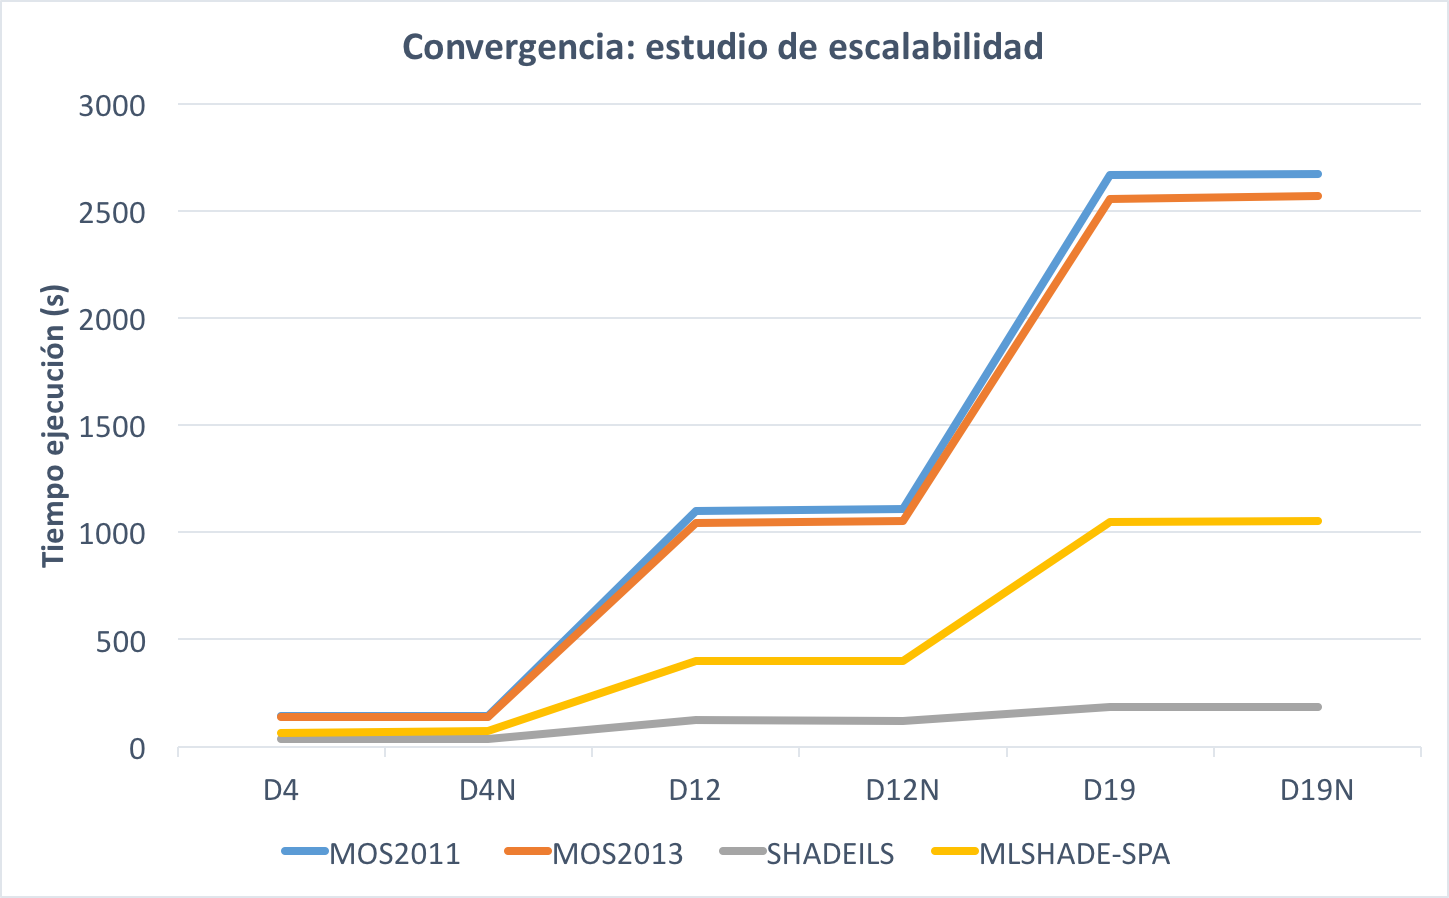
\includegraphics[scale=0.52]{imagenes/ConvergenciaEscalabilidad}
	\caption{Convergencia temporal de los 4 algoritmos para cada problema}
\end{figure}\label{fig:ConvergenciaEscalabilidad}


Atendiendo a los resultados obtenidos para los tres experimentos conducidos con DG2, se puede comprobar que el escenario obtenido no es el más indicado como para abordar el problema mediante una descomposición de variables: la salida del algoritmo, además de mostrar el excesivo tiempo de computación que emplea, muestra que no es posible realizar una descomposición del problema debido a que la función es no separable. Este escenario puede tener como explicación una razón, donde la propia naturaleza del problema puede marcar el camino del algoritmo sin necesidad de una ejecución posterior.

Como se explica en la introducción al problema, en un EEG real las señales se combinan debido a \textit{interferencias y ruido} propios de la medición, lo que hace que un electrodo \textbf{i} pueda medir información tanto local a su zona como la que se produce en otras zonas que \textbf{también} están siendo medidas por otros electrodos \textbf{k}. De esta forma, la interacción de las variables es máxima, como se puede ver en este caso, lo que limita considerablemente las capacidades del algoritmo, al no ser capaz de obtener una descomposición óptima que \textbf{minimice} la interacción entre componentes, por el simple y llano hecho de que no existe descomposición posible.

Teniendo en cuenta estos resultados y la primitiva que se expresa en \cite{DG}, la técnicas de Cooperación Co-evolutiva dedicadas a optimizar funciones no-separables de alta dimensionalidad no han mostrado resultados suficientemente competentes como para ser considerados aplicables en un ámbito real donde no se tiene información alguna acerca de la interacción de las variables de la función. A esto hay que añadirle el hecho de que los más recientes estudios de CC con descomposición de variables han sido probados con funciones separables o parcialmente separables, por lo que en gran medida se desconoce la escalabilidad de estas propuestas en funciones no-separables\cite{DG}.

Estas circunstancias motivan la decisión de \textbf{no continuar con DG2} para la fase de experimentación completa, dado que el \textbf{resultado} se torna \textbf{incierto} desde un principio y que además, las restricciones temporales inherentes al problema no pueden contemplar que una técnica híbrida que se pretende aplicar en un campo u entorno real, tenga un tiempo de respuesta superior a las \textbf{doce horas}, como es el caso de la función del EEG en el problema D12.

Teniendo en cuenta esta situación, se hace impensable la aplicación de este tipo de técnicas para optimizar un encefalograma actual que puede disponer de más de \textbf{20 señales de entrada e innumerable artifacts}, con una frecuencia de muestreo superior a la de este benchmark sintético. A partir de este punto, queda totalmente descartada la aplicación de este algoritmo en los posteriores experimentos de este estudio, por lo que tampoco se tendrá en consideración en las conclusiones finales, en cuanto a propuesta de solución real se refiere. Se procede con la fase de experimentación completa.


\section{Estudio experimental completo}\label{sect:FE2}

El estudio experimental completo muestra los resultados de 10 ejecuciones de cada algoritmo para cada uno de los 6 problemas de dimensionalidad que proponer el benchmark del EEG. En esta fase, se miden características como los valores \textbf{mínimos y máximos} de fitness alcanzados por cada algoritmo a lo largo de las 10 ejecuciones, así como una \textbf{media del fitness global} y donde, en esta ocasión, se muestra el \textbf{tiempo medio} transcurrido teniendo en cuenta la totalidad de las ejecuciones realizadas. 

En este estudio se ha utilizado un número de \textbf{evaluaciones de la función objetivo}, que es el criterio de parada, igual a 1 millón (1M); se ha elegido este valor en función de los resultados de la gráfica de convergencia destacada con anterioridad y por la escalabilidad en cuanto al tiempo de ejecución de los algoritmos. Para cada una de las técnicas, se muestra una tabla con valores \textbf{mínimos}, \textbf{máximos} y \textbf{medios de fitness} tras las 10 ejecuciones, así como el \textbf{tiempo de ejecución medio}. 

Resaltar que teniendo en cuenta que muchas de las \textbf{diferencias de valores fitness} entre los distintos algoritmos se producen más allá de las 10 cifras decimales, es posible encontrarse valores iguales tanto para mínimo, máximo y media para distintos algoritmos, fenómeno que no ocurre para las medias temporales. Posteriormente se mostrará una tabla resumen de fitness medio y tiempo medio, junto con el algoritmo de referencia, momento a partir del cual se comenzará el análisis de los resultados.

\begin{enumerate}
	\item \textbf{MOS2011}:
			
			\begin{table}[H]
				\centering
				\resizebox{\textwidth}{!}{
					$\begin{tabular}{ *{5}{c}}
					\toprule
					\textbf{Problema} & \textbf{Min.}  & \textbf{Max.} & \textbf{Media} & \textbf{Tiempo} \\
					\midrule
						D4 & 0.06103 & 0.06103 & 0.06103 & 1519.903\\ 
						D4N & 0.05897 & 0.05897 & 0.05897 & 1567.199\\ 
						D12 & 0.00194 & 0.00200 & 0.00198 & 12634.289\\ 
						D12N & 0.00187 & 0.00190 & 0.00188 & 12593.868\\ 
						D19 & 0.00830 & 0.00992 & 0.00894 & 28033.663\\ 
						D19N & 0.00824 & 0.00978 & 0.00918 & 28586.774\\ 
					\bottomrule
					\end{tabular}$
				}
					\caption{Resultados MOS2011: Experimentación completa}
					\label{tabla:ResMOS2011-Exp2}
			\end{table}
		
		\item \textbf{MOS2013}:
		
		\begin{table}[H]
			\centering
			\resizebox{\textwidth}{!}{
				$\begin{tabular}{ *{5}{c}}
				\toprule
				\textbf{Problema} & \textbf{Min.}  & \textbf{Max.} & \textbf{Media} & \textbf{Tiempo} \\
				\midrule
					D4 & 0.06103 & 0.06103 & 0.06103 & 1265.065\\ 
					D4N & 0.05897 & 0.05897 & 0.05897 & 1221.990\\ 
					D12 & 0.00194 & 0.00194 & 0.00194 & 9597.190\\ 
					D12N & 0.00183 & 0.00183 & 0.00183 & 9520.520\\ 
					D19 & 0.00251 & 0.00251 & 0.00251 & 23524.796\\ 
					D19N & 0.00256 & 0.00256 & 0.00256 & 23037.743\\ 
				\bottomrule
				\end{tabular}$
			}
				\caption{Resultados MOS2013: Experimentación completa}
				\label{tabla:ResMOS2013-Exp2}
		\end{table}
	\newpage
	\item \textbf{SHADEILS}:
	
		\begin{table}[H]
		\centering
		\resizebox{\textwidth}{!}{
			$\begin{tabular}{ *{5}{c}}
			\toprule
			\textbf{Problema} & \textbf{Min.}  & \textbf{Max.} & \textbf{Media} & \textbf{Tiempo} \\
			\midrule
				D4 & 0.06103 & 0.06103 & 0.06103 & 251.759\\ 
				D4N & 0.05897 & 0.05897 & 0.05897 & 250.908\\ 
				D12 & 0.00194 & 0.00194 & 0.00194 & 802.331\\ 
				D12N & 0.00183 & 0.00183 & 0.00183 & 786.965\\ 
				D19 & 0.00251 & 0.00252 & 0.00252 & 1578.034\\ 
				D19N & 0.00256 & 0.00256 & 0.00256 & 1573.507\\ 
			\bottomrule
			\end{tabular}$
		}
			\caption{Resultados SHADEILS: Experimentación completa}
			\label{tabla:ResSHADEILS-Exp2}
	\end{table}

	\item \textbf{MLSHADE-SPA}:

	\begin{table}[H]
		\centering
		\resizebox{\textwidth}{!}{
			$\begin{tabular}{ *{5}{c}}
			\toprule
			\textbf{Problema} & \textbf{Min.}  & \textbf{Max.} & \textbf{Media} & \textbf{Tiempo} \\
			\midrule
				D4 & 0.06103 & 0.06103 & 0.06103 & 490.294\\ 
				D4N & 0.05897 & 0.05897 & 0.05897 & 487.606\\ 
				D12 & 0.00194 & 0.00194 & 0.00194 & 3918.041\\
				D12N & 0.00183 & 0.00183 & 0.00183 & 3936.233\\ 
				D19 & 0.00252 & 0.00252 & 0.00252 & 9229.300\\ 
				D19N & 0.00256 & 0.00256 & 0.00256 & 8595.423\\ 
			\bottomrule
			\end{tabular}$
		}
			\caption{Resultados MLSHADE-SPA: Experimentación completa}
			\label{tabla:ResMLSHADESPA-Exp2}
	\end{table}
	
\end{enumerate}


\section{Comparativa Global}

La tabla resumen que se muestra a continuación permite obtener una visión global de los resultados, además de permitir comparar con el algoritmo de referencia \textbf{MAGA}\cite{MAGA-BigOpt}. En esta se aprecia el valor de fitness medio tras las 10 ejecuciones del algoritmo para cada problema. Tras discutir los resultados obtenidos en cuanto a valores fitness, se procederá con al análisis teniendo en cuenta el tiempo de ejecución.

\begin{table}[H]
	\centering
	\resizebox{\textwidth}{!}{
		$\begin{tabular}{ *{7}{c}}
		\toprule
		\textbf{Algoritmo} & \textbf{D4}  & \textbf{D4N} & \textbf{D12} & \textbf{D12N} & \textbf{D19} & \textbf{D19N}\\
		\midrule
		MOS2011 & 0.06103 & 0.05897 & 0.00198 & 0.00188 & 0.00894 & 0.00918\\ 
		MOS2013 & 0.06103 & 0.05897 & 0.00194 & 0.00183 & 0.00251 & 0.00256\\ 
		MLSHADE-SPA & 0.06103 & 0.05897 & 0.00194 & 0.00183 & 0.00252 & 0.00256\\ 
		SHADEILS & 0.06103 & 0.05897 & 0.00194 & 0.00183 & 0.00252 & 0.00256\\
		MAGA* & 0.0610 & 0.0590 & 0.0019 & 0.0018 & 0.0025 & 0.0026\\ 
		\bottomrule
		\end{tabular}$
	}
	\caption{Valores fitness medio. MAGA*: algoritmo de referencia.}
	\label{tabla:ResumenFitness}
\end{table}

A partir de los resultados obtenidos podemos deducir las siguientes conclusiones generales:

\begin{itemize}
	\item El problema \textbf{D4} (1024 variables) puede parecer más complejo de resolver a priori, en cuanto a valor fitness se refiere. Sin embargo lo que realmente ocurre es que se dispone de \textbf{menos información} - menor cantidad de señales mezcladas - de las que el algoritmo necesita para identificar la correlación entre las señales y separar los artifacts de la misma. Si además se tiene en cuenta que en un problema médico real en el que intervenga un electroencefalograma es común encontrar al menos \textbf{20 electrodos}, que actuarían como fuentes de señales, este problema no es representativo de cara a un entorno real.
	
	\item El problema \textbf{D12} (3072 variables) presenta los mejores resultados y eso se debe al equilibrio entre cantidad de información disponible y capacidad de las técnicas actuales. A pesar de crecer en términos de dimensionalidad, la calidad de las soluciones es mejor porque precisamente se dispone de mayor cantidad de información para que el algoritmo calcule la matriz \textbf{S1} con una precisión mayor que para el problema anterior. 
	
	Además cabe destacar en este punto la flexibilidad y robustez de las técnicas elegidas, debido a que a pesar de haber sido diseñadas para un benchmark cuya dimensionalidad es de 1000 variables, no pierden capacidad de convergencia frente a una dimensionalidad  3 veces mayor, llegando incluso a mostrar ajustes mejores que con menor cantidad de información. En cualquier caso, sigue siendo precipitado considerar este problema como \textit{suficientemente representativo} de un problema de optimización de un EEG real, a pesar de si ser mas representativo que el anterior.
	
	\item El problema \textbf{D19} (4864 variables) muestra como afecta la dimensionalidad del problema en la calidad de las soluciones. A pesar de alcanzar resultados bastante más satisfactorios en comparación con D4, la elevada dimensionalidad hace que a pesar de contener más información representativa para identificar la correlación entre las señales, el algoritmo no sea capaz (en términos de potencia) de obtener mejores soluciones que con menos variables. Sin embargo, se dispone de argumentos suficientes como para afirmar que las propuestas de algoritmos elegidas son \textbf{escalables}: al cambiar de benchmark han respondido de forma satisfactoria; un indicador más de la robustez de las técnicas empleadas.
	
	\item El algoritmo de referencia \textbf{MAGA} que se utiliza en esta comparativa es una técnica que, como anteriormente se ha expuesto, ha evolucionado de su antecesora y ha sido diseñada exclusivamente para la resolución del benchmark del EEG. Tomando en consideración este precepto, podemos comprobar como todos los algoritmos menos \textbf{MOS2011} (en problemas de dimensionalidad mayor, principalmente) muestran resultados prácticamente idénticos que el algoritmo de referencia, lo que es un buen indicador, nuevamente, de la potencia de estos algoritmos y las capacidades de hacer frente a problemas muy distintos.
	
	\item Finalmente, destacar que la introducción de ruido en los problemas (de varianza 0.1) no es lo suficientemente relevante como para causar un detrimento en la calidad de las soluciones, donde tampoco se ve afectado de forma significativa el tiempo de ejecución medio de los algoritmos, por lo que es importante destacar que la formulación del benchmark elegida no es la más adecuada en términos de ruido añadido, ya que no añade suficiente dificultad durante el proceso de optimización.
\end{itemize}

Tomando como referencia la tabla resumen de fitness medio (tabla \ref{tabla:ResumenFitness}), se puede comprobar como \textbf{MOS2013} introduce una mejora sustancial al cambiar el diseño del algoritmo, mejora que se hace más notable conforme crece la dimensión del problema, llegando a reducir el error obtenido en los problemas D19(N) en alrededor de un 25\% . A pesar de que la implementación de MOS2011 utiliza un algoritmo de evolución diferencial (DE) que es más escalable que el algoritmo genético clasico de MOS2013, los métodos de búsqueda local empleados por MOS2013 son mucho más potentes y rápidos, lo que le otorga a este una velocidad de convergencia superior a la de su predecesor. 

Destacar en este punto la implementación de la \textbf{MTS-LS1-Reduced} utilizada en MOS2013, donde en vez de explorar todas las variables a la vez, se centra en aquellas que más aportan a la mejora de la calidad de las soluciones, optimizando al máximo la cantidad de evaluaciones de la función objetivo a la vez que reduce la dimensión de las operaciones que realiza, otorgándole a MOS2013 mayor velocidad de convergencia, lo que se nota de forma indiscutible en las dimensiones más altas.

Si se consideran las implementaciones de \textbf{MOS2013}, \textbf{SHADEILS} y \textbf{MLSHADE-SPA} es fácilmente reconocible la potencia de las tres técnicas en comparación con MOS2011, sobretodo conforme crece la dimensionalidad del problema. Partiendo de la base de que se disponen de técnicas muy robustas y escalables, que además han mostrado rendimientos prácticamente idénticos, tanto entre ellas como con el algoritmo de referencia MAGA, se torna indispensable utilizar otro enfoque de comparativa: el \textbf{enfoque temporal}. Teniendo en cuenta que los resultados están supeditados a los tiempos de respuesta efectiva de los algoritmos, se procede a comparar las propuestas de este estudio utilizando la característica temporal, detallando en primera instancia 

\begin{table}[h]
	\centering
	\resizebox{\textwidth}{!}{
		$\begin{tabular}{ *{7}{c}}
		\toprule
		\textbf{Algoritmo} & \textbf{D4}  & \textbf{D4N} & \textbf{D12} & \textbf{D12N} & \textbf{D19} & \textbf{D19N}\\
		\midrule
		MOS2011 & 1519 & 1567 & 12634 & 12593 & 28033 & 28586\\ 
		MOS2013 & 1265 & 1221 & 9597 & 9520 & 23524 & 23037\\ 
		MLSHADE-SPA & 490 & 487& 3918 & 3936 & 9229 & 8595\\ 
		SHADEILS & 251 & 250 & 802 & 786 & 1578 & 1573\\
		\bottomrule
		\end{tabular}$
	}
	\caption{Tiempo medio (s) }
	\label{tabla:ResumenTiempo}
\end{table}


 Se parte de la idea de que, como es natural, los tiempos de ejecución están determinados por el número de variables: a mayor tamaño del espacio de soluciones, mayor cantidad de operaciones hay que realizar y más costosas se tornan estas operaciones. El ruido introducido en este benchmark, de forma sintética, no afecta de forma significativa alguna al tiempo de respuesta, llegando en ocasiones incluso a \textit{facilitar} (véase la tabla \ref{tabla:ResumenTiempo}) la convergencia del algoritmo en términos temporales. Por último,  destacar el \textbf{aumento no lineal} de los tiempos de ejecución en función del número de variables, lo que reafirma la incapacidad de obtener información alguna acerca de la correlación entre las variables de cara a una implementación híbrida de técnicas que requieran descomposiciones lo más óptimas posibles para alcanzar resultados competitivos.
 
 La tabla de porcentajes de tiempos que se muestra a continuación, que no es más que un resumen en representación porcentual de la tabla \ref{tabla:ResumenTiempo}, muestra el porcentaje de reducción temporal de cada una de las técnicas con respecto a la propuesta más lenta, en este caso, MOS2011.
 
 \begin{table}[h]
 	\centering
 	\resizebox{\textwidth}{!}{
 		$\begin{tabular}{ *{7}{c}}
 		\toprule
 		\textbf{Algoritmo} & \textbf{D4}  & \textbf{D4N} & \textbf{D12} & \textbf{D12N} & \textbf{D19} & \textbf{D19N}\\
 		\midrule
 		MOS2011 & 100 & 100 & 100 & 100 & 100 & 100\\ 
 		MOS2013 & 83 & 77 & 75 & 75 & 83 & 80\\ 
 		MLSHADE-SPA & 32 & 31& 31 & 31 & 32 & 30\\ 
 		SHADEILS & 16 & 15 & 6 & 6 & 6 & 5\\
 		\bottomrule
 		\end{tabular}$
 	}
 	\caption{Porcentaje (\%) de reducción temporal }
 	\label{tabla:ResumenTiempoPorcentaje}
 \end{table}

A través de esta tabla se puede comprobar como \textbf{MOS2013} tiene un mejor tiempo de respuesta que su antecesor MOS2011. Las técnicas de búsqueda locales empleadas por este son más potentes que las de su predecesor, lo que se traduce también en un tiempo de respuesta menor: MOS2013 consigue reducir los tiempos de ejecución entre un 20\% y 25\% con respecto a MOS2011 para la totalidad de los problemas.

En cuanto al segundo mejor, en términos temporales, \textbf{MLSHADE-SPA} tiene un rendimiento destacable frente a las dos propuestas MOS. Emplea alrededor de un 30\% del tiempo que necesita MOS2011 y menos de la mitad del que requiere MOS2013, llegando a resolver el problema de dimensión D12 en una hora en vez de 3, al igual que emplea de media algo menos de 3 horas en resolver el problema D19, tiempo que en MOS2013 se va hasta rozar las 8 horas de ejecución.

A grandes rasgos, queda muy claro que \textbf{SHADEILS} es el mejor de todos los algoritmos en relación calidad de la solución - tiempo de ejecución, donde se mantiene a menos de un 10\% del tiempo de ejecución que emplea MOS2011 para los problemas D12(N) y D19(N). La diferencia con MOS2013 es un poco menos significativa, en torno a un 12.5\% de media para todos los problemas, y cerca de un 20\% del tiempo con respecto a MLSHADE-SPA para dimensiones D12 y D19, situándose como claro vencedor en esta comparativa dado que es \textbf{único algoritmo} que ha conseguido resolver todos los problemas en menos de media hora.


Sin embargo, estos resultados pueden parecer contradictorios a priori debido a la \textbf{naturaleza de las implementaciones} y de las \textbf{tecnologías empleadas}. Es bien sabido que \textbf{C++ y C} son los lenguajes de programación \textbf{más rápidos} de la actualidad, dada su condición de \textit{compilados}. Seguidamente, otros lenguajes como pueden ser en este caso \textbf{Python} o \textbf{MATLAB} quedan forzosamente por detrás de C++ al ser lenguajes interpretados. Surge entonces la pregunta de cómo una implementación en un lenguaje compilado, como las de MOS2011 y MOS2013, es ordenes de magnitud \textbf{más lenta} que una implementación en un lenguaje interpretado, como las de SHADEILS y MLSHADE-SPA.

La respuesta está en el diseño de cada una de las técnicas. Mientras que tanto MOS2011 como MOS2013 utilizan la librería \textbf{GAlib}, que a grandes rasgos no es más que un conjunto de plantillas para diseñar algoritmos evolutivos, pero que añade mucha complejidad estructural al algoritmo además de la propia que ya introduce el diseño del algoritmo en cuanto a parámetros propios y las operaciones que efectúa, SHADEILS hace un uso intensivo de librerías como \textbf{Numpy}, que permiten acceder desde Python a implementaciones robustas y optimizadas de operaciones en C++, consiguiendo un resultado en cuanto a tiempo de respuesta muy similar al que se obtendría si se utilizase C++ de forma nativa.

Siguiendo con el diseño, MOS utiliza algoritmos evolutivos clásicos como el \textbf{GA}, cuya escalabilidad es muy baja, lo que aumenta considerablemente el tiempo de ejecución. Por otra parte, tanto SHADEILS como MLSHADE-SPA hacen uso intensivo de técnicas muy avanzadas de evolución diferencial, como lo es \textbf{SHADE} o \textbf{L-SHADE}, esta última presente en MLSHADE-SPA donde aplica una reducción gradual de la población. Aunque no es posible saber con certeza si un tamaño de población que se reduce constantemente pueda ser indicativo de una mejora en el tiempo de respuesta, como es el caso si se comparan MOS y MLSHADE-SPA, hay que tener en cuenta que SHADEILS utiliza apenas un cuarto de la población de MOS2013, lo que si puede ser indicativo de una mejora sustancial de un algoritmo a otro.

Dada la implementación particular de cada técnica y los resultados obtenidos al utilizar distintos lenguajes de programación, se puede afirmar que si se implementasen todas las técnicas en un mismo lenguaje, prevalecerían los resultados que se han obtenido en este estudio, consiguiendo reducir aún más los tiempos de ejecución de algoritmos como SHADEILS o MLSHADE-SPA. 

No obstante, si ahora se compara a SHADEILS con el algoritmo de referencia \textbf{MAGA}, los resultados no parecen ser tan competitivos. MAGA es un algoritmo que ha sido diseñado expresamente para este benchmark, por lo que no se tienen registros algunos de resultados con otros benchmarks del panorama LSGO. Además, el autor de la publicación no refleja el criterio de parada del algoritmo ni la cantidad de evaluaciones de la función objetivo que ejecuta, por lo que se ha tomado la decisión de medir el tiempo que tarda \textbf{SHADEILS} en alcanzar una \textbf{precisión igual} a la que se muestra en el algoritmo de referencia en cuanto a valor fitness, para así poder comparar ambos algoritmos bajo condiciones similares.

Para ello, se ha ejecutado SHADEILS para cada problema con una semilla aleatoria y 1 millón de evaluaciones de la función objetivo. La tabla correspondiente se muestra a continuación, donde los valores fitness de referencia que se han utilizado para esta experimentación en concreto son los que aparecen en la tabla \ref{tabla:ResumenFitness}.

\begin{table}[h]
	\centering
	\resizebox{\textwidth}{!}{
		$\begin{tabular}{ *{7}{c}}
		\toprule
		\textbf{Algoritmo} & \textbf{D4}  & \textbf{D4N} & \textbf{D12} & \textbf{D12N} & \textbf{D19} & \textbf{D19N}\\
		\midrule 
		SHADEILS & 1.152 & 0.934 & 47.175 & 47.759 & 472.229 & 472.010\\ 
		MAGA & 0.190 & 0.191 & 1.322 & 1.396 & 7.176 & 9.216\\ 
		\bottomrule
		\end{tabular}$
	}
	\caption{Tiempo (s) de SHADEILS en conseguir un error igual a MAGA }
	\label{tabla:ResumenMAGA-SHADEILS}
\end{table}

Los datos muestran que SHADEILS tiene una velocidad de convergencia alta, hecho que queda demostrado tras haber medido el tiempo transcurrido hasta que se alcanza por primera vez la solución optima de MAGA. Si se tiene en consideración que el autor de la publicación ha utilizado Visual Studio 2010 y Windows 7 para la implementación de la propuesta\cite{MAGA-BigOpt}, es posible que también haya utilizado C++ para la implementación del algoritmo. Tomando en cuenta las consideraciones expresadas anteriormente en cuanto a la mejora de tiempo que se conseguiría al trasladar la implementación de los algoritmos de MATLAB y Python (MLSHADE-SPA y SHADEILS respectivamente) existe una alta probabilidad de que los tiempos de respuesta de estos algoritmos también mejoren, lo que reduciría las distancias actuales entre SHADEILS y MAGA, situando al primero de estos en una muy buena posición con respecto a sus demás competidores.

Llegados a este punto es apropiado afirmar que las propuestas elegidas en este estudio han mostrado resultados competitivos. Aún así se puede concluir que son necesarias técnicas no más potentes pero si \textbf{más rápidas} para permitir su aplicación sobre problemas de optimización en ámbitos reales. El campo LSGO es un área de conocimiento que ha nacido relativamente hace poco y hasta hace apenas tres años, la gran mayoría de propuestas se remitían únicamente a los congresos, conferencias y competiciones, siendo estudiadas y evaluadas sobre benchmarks poco representativos del panorama del LSGO del mundo real. 

Sin embargo, durante los últimos tres años se han propuesto una mayor cantidad de técnicas y algoritmos en este campo de estudio, lo que indudablemente promoverá su crecimiento y evolución de forma notable. Además, permitirá que sea solo cuestión de tiempo que se propongan técnicas mucho más sofisticadas y potentes que lleguen a ser aplicables a un problema real, repercutiendo en una mejora de la calidad de los procesos que requieren optimización y por ende afectando de forma positiva al entorno social donde son implantadas.












 %parte experimental
\chapter{Conclusiones y posibles extensiones}\label{cap:Conclusiones}

En este trabajo se ha estudiado cómo es el rendimiento y la escalabildad de las propuestas más novedosas y potentes del panorama de optimización en alta dimensionalidad. Para lograr este objetivo, se ha utilizado un benchmark con una formulación de un problema totalmente distinto a los que se proponen en los benchmarks más utilizados actualmente: la optimización de los datos de un electroencefalograma en un ámbito médico real.

Se han estudiado el diseño de estas propuestas y se han adaptado las mismas para ser capaces de procesar la función objetivo del problema propuesto, lo que derivaría en la posterior obtención de los resultados, a través de un proceso de experimentación exhaustivo, que servirían de base para sustentar la posible utilidad de estas técnicas de cara a una implantación en un entorno real.

Los resultados han sido analizados y se concluye que las técnicas elegidas del ámbito \textit{large scale global optimization} son muy robustas, escalables y potentes. Sin embargo, aún queda un largo camino por recorrer en materia LSGO, donde el principal inconveniente sigue siendo los excesivos tiempos de ejecución de estos algoritmos, aunque como se ha visto, distintas implementaciones utilizando distintas tecnologías podrían ser capaces de resolver estas deficiencias.

A criterio del alumno, no se conoce en la literatura actual del panorama de optimización en alta dimensionalidad un trabajo como el que se presenta en estas páginas. Es este precepto el que motivó la realización del mismo, donde se propone una hoja de ruta a seguir en cuanto a la optimización del problema del electroencefalograma se refiere, lo que puede derivar, ya sea a corto-medio o largo plazo, en una mejora sustancial de las técnicas empleadas actualmente para su optimización, lo que se traduciría en un uso mucho más extensivo y eficiente en determinadas áreas de conocimiento y para determinadas aplicaciones que así lo requieran.

Como posibles extensiones de este trabajo se propone un ajuste exhaustivo y extensivo de los parámetros de cada algoritmo siguiendo el enfoque del benchmark estudiado en este trabajo, con vistas a conseguir una posible mejora de las soluciones obtenidas. De forma análoga, la inclusión de más benchmarks formulados a partir de problemas reales aumentaría la diversidad de los estudios, lo que podría llevar a mejorar el rendimiento de las técnicas actuales.

Ampliar el presente estudio con más técnicas también puede formar parte de una extensión futura, donde se añadan implementaciones en lenguajes más eficientes de cara a preparar las propuestas a un entorno real donde las restricciones temporales juegan un papel clave. Realizar una mejora del propio benchmark del EEG con el fin de que sea más representativo de un problema médico real, añadiendo más variables y mayor ruido, para crear mayor incertidumbre y forzar a que las técnicas que busquen su resolución sean cada vez más sofisticadas, se considera también una posible extensión de este trabajo.

Concluye así por tanto este estudio, donde el alumno agradece toda la ayuda proporcionada por la institución en cuanto a los recursos para llevar a cabo este trabajo, así como al tutor del mismo por el apoyo condicional y por guiar el buen desarrollo de este Trabajo Fin de Grado.


\nocite{*}
\bibliography{bibliografia/bibliografia}\addcontentsline{toc}{chapter}{Bibliografía}
\bibliographystyle{unsrt}
%
\appendix
\chapter{Gráficas de convergencia del estudio de escalabilidad}


\begin{figure}[H]
	\centering
	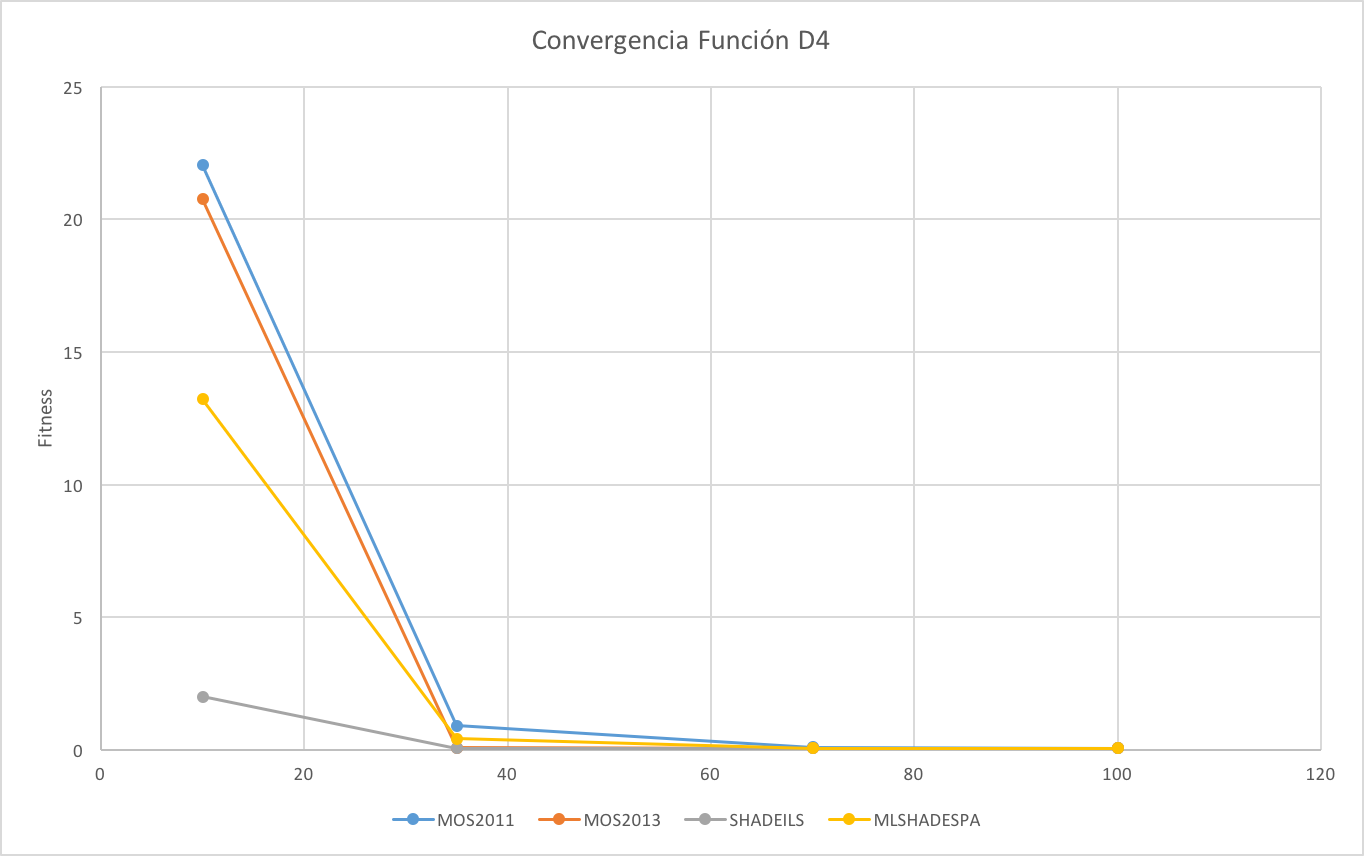
\includegraphics[scale=0.6]{imagenes/ConvergenciaD4}
	\caption{Convergencia de los 4 algoritmos: problema D4}
	\label{fig:ConvgD4}
\end{figure}

\begin{figure}[H]
	\centering
	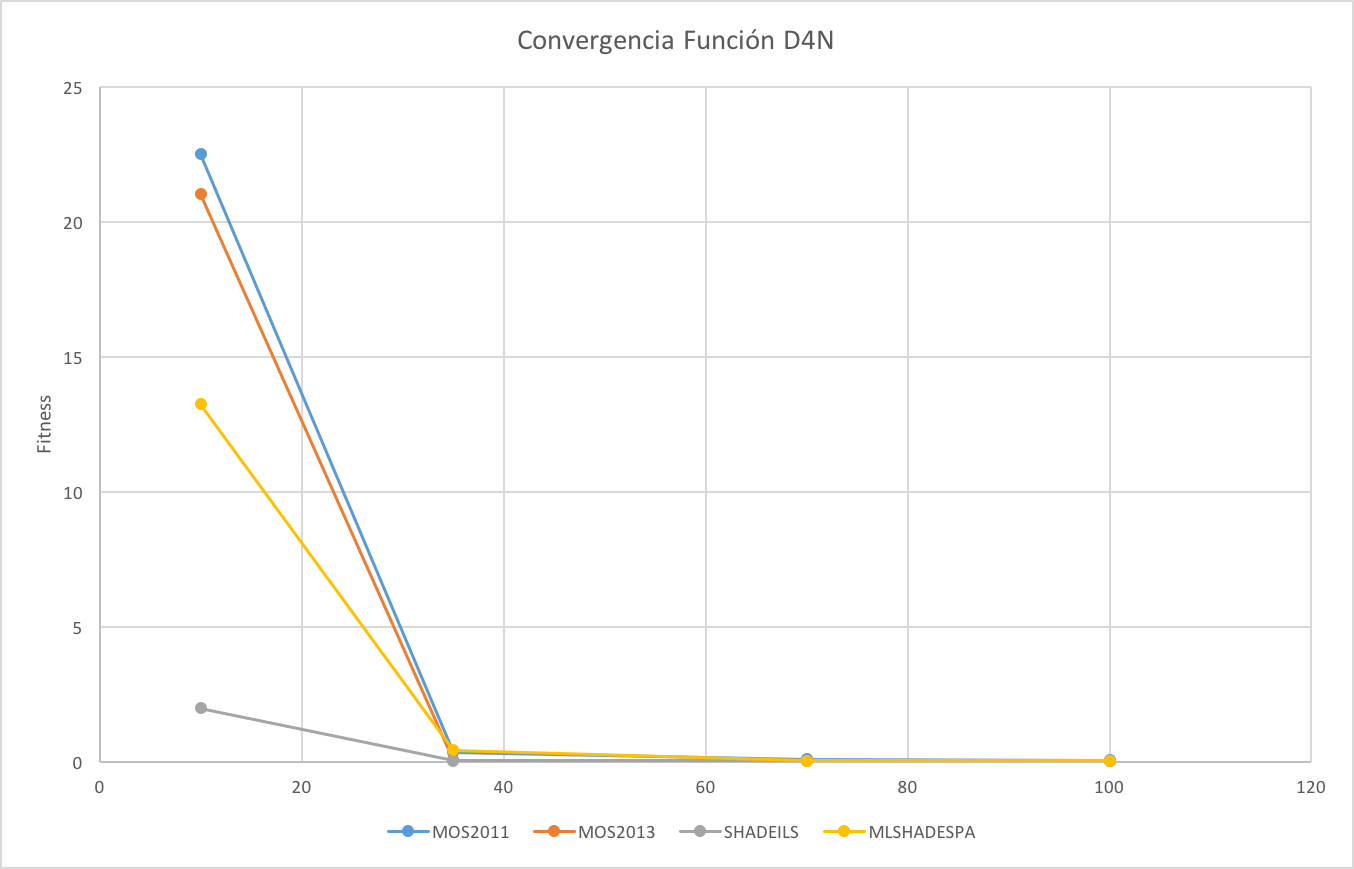
\includegraphics[scale=0.6]{imagenes/ConvergenciaD4N}
	\caption{Convergencia de los 4 algoritmos: problema D4N}
	\label{fig:ConvgD4N}
\end{figure}

\begin{figure}[H]
	\centering
	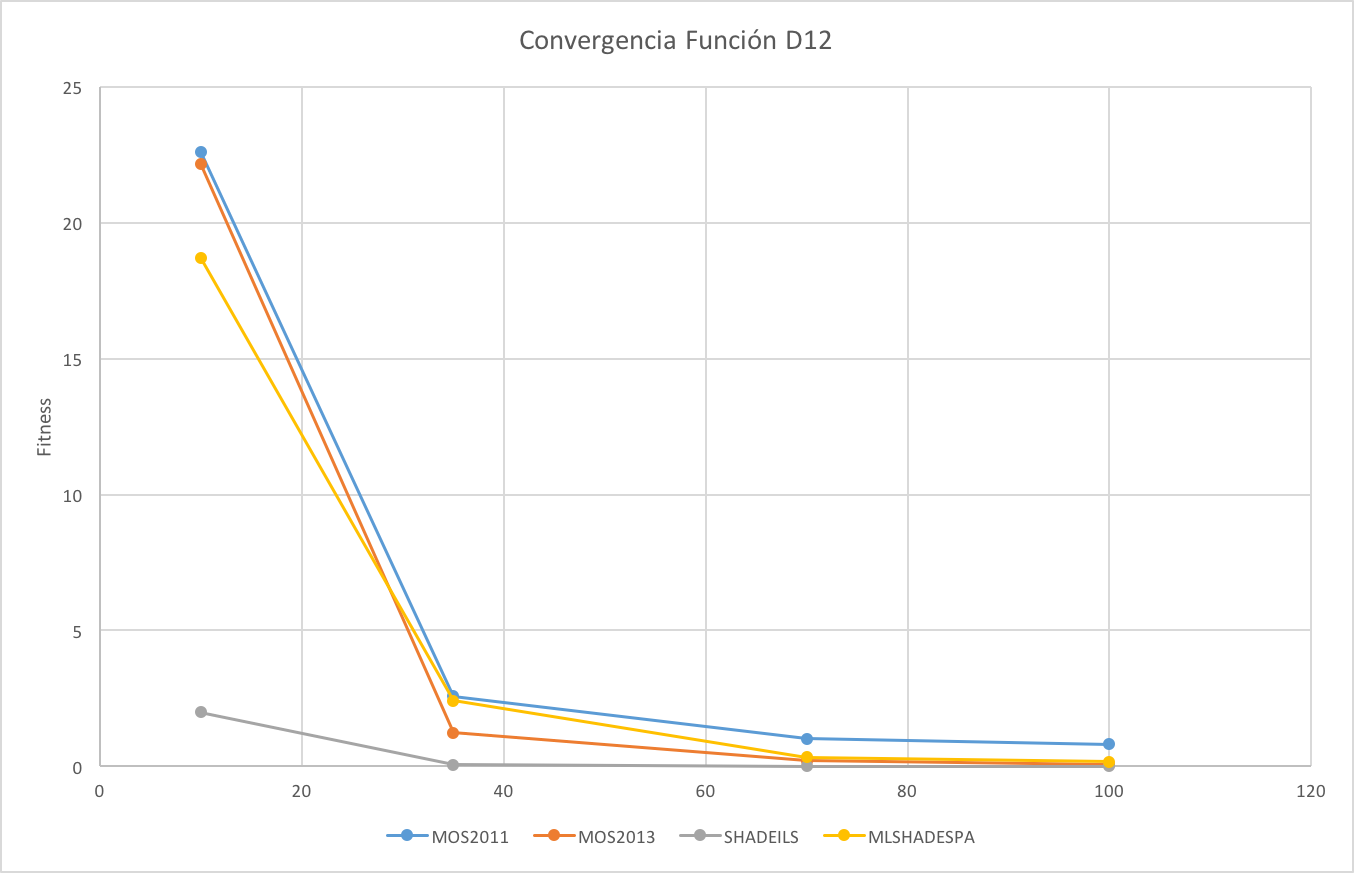
\includegraphics[scale=0.6]{imagenes/ConvergenciaD12}
	\caption{Convergencia de los 4 algoritmos: problema D12}
	\label{fig:ConvgD12}
\end{figure}

\begin{figure}[H]
	\centering
	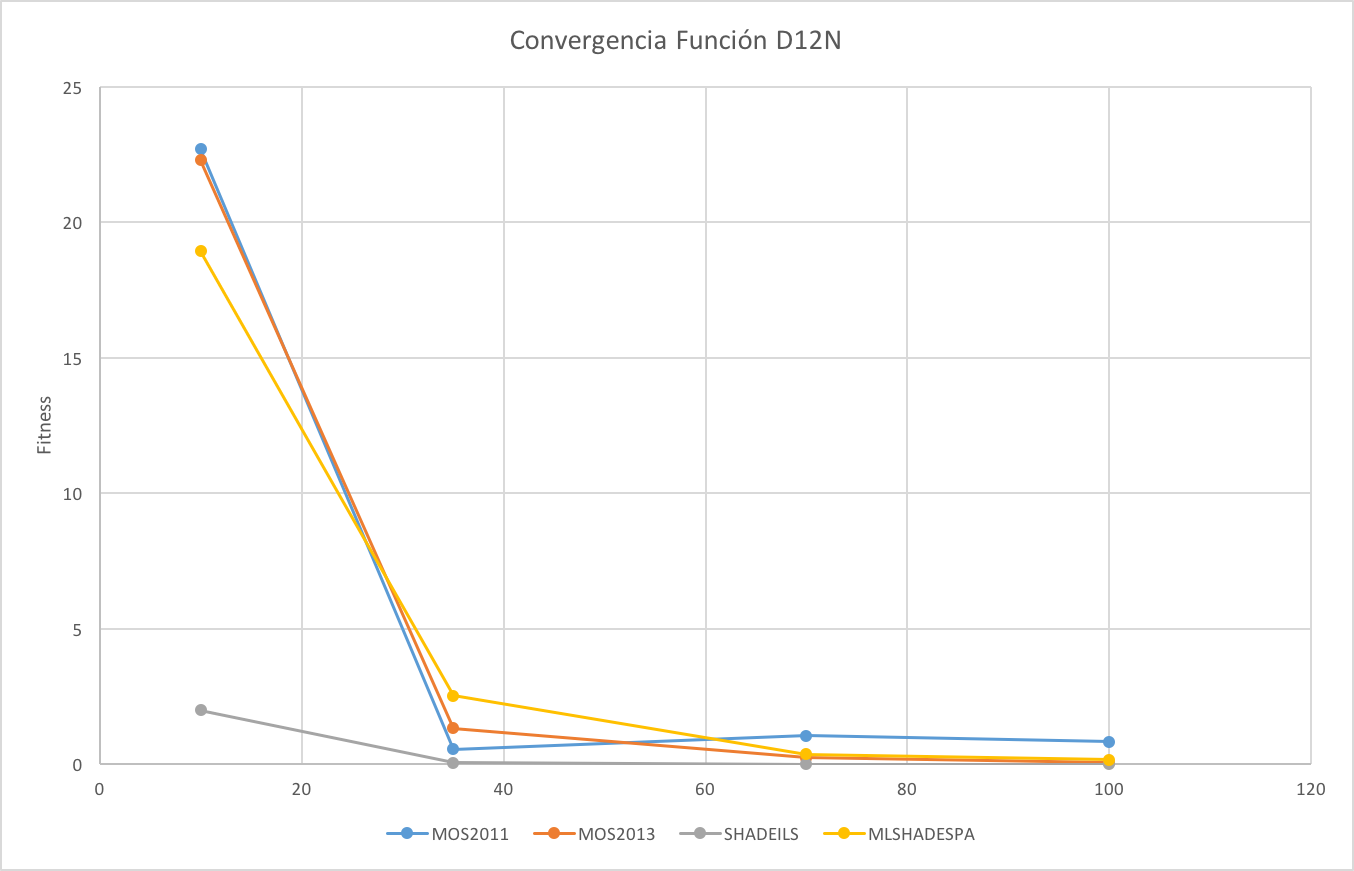
\includegraphics[scale=0.6]{imagenes/ConvergenciaD12N}
	\caption{Convergencia de los 4 algoritmos: problema D12N}
	\label{fig:ConvgD12N}
\end{figure}

\begin{figure}[H]
	\centering
	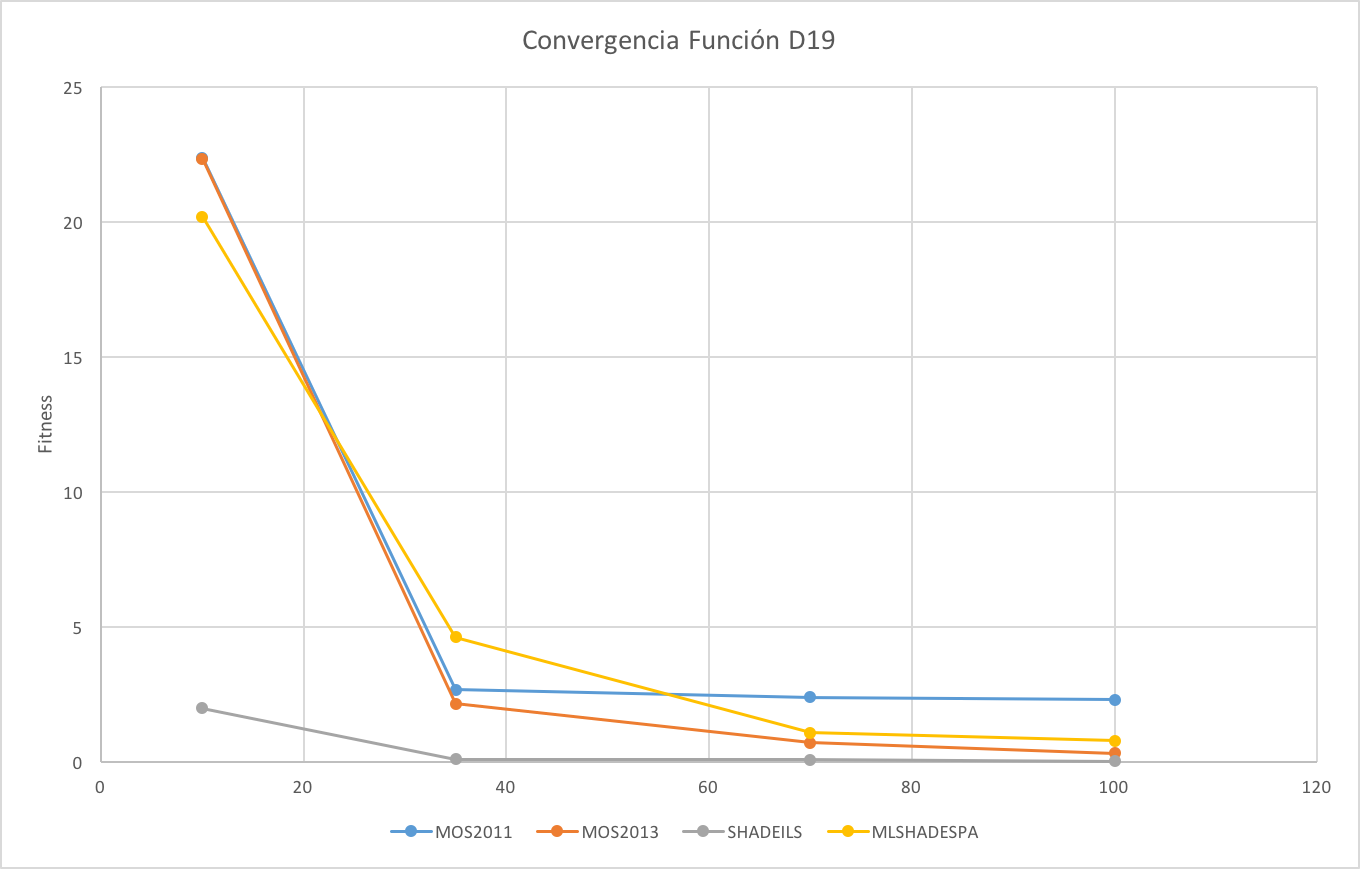
\includegraphics[scale=0.6]{imagenes/ConvergenciaD19}
	\caption{Convergencia de los 4 algoritmos: problema D19}
	\label{fig:ConvgD19}
\end{figure}

\begin{figure}[H]
	\centering
	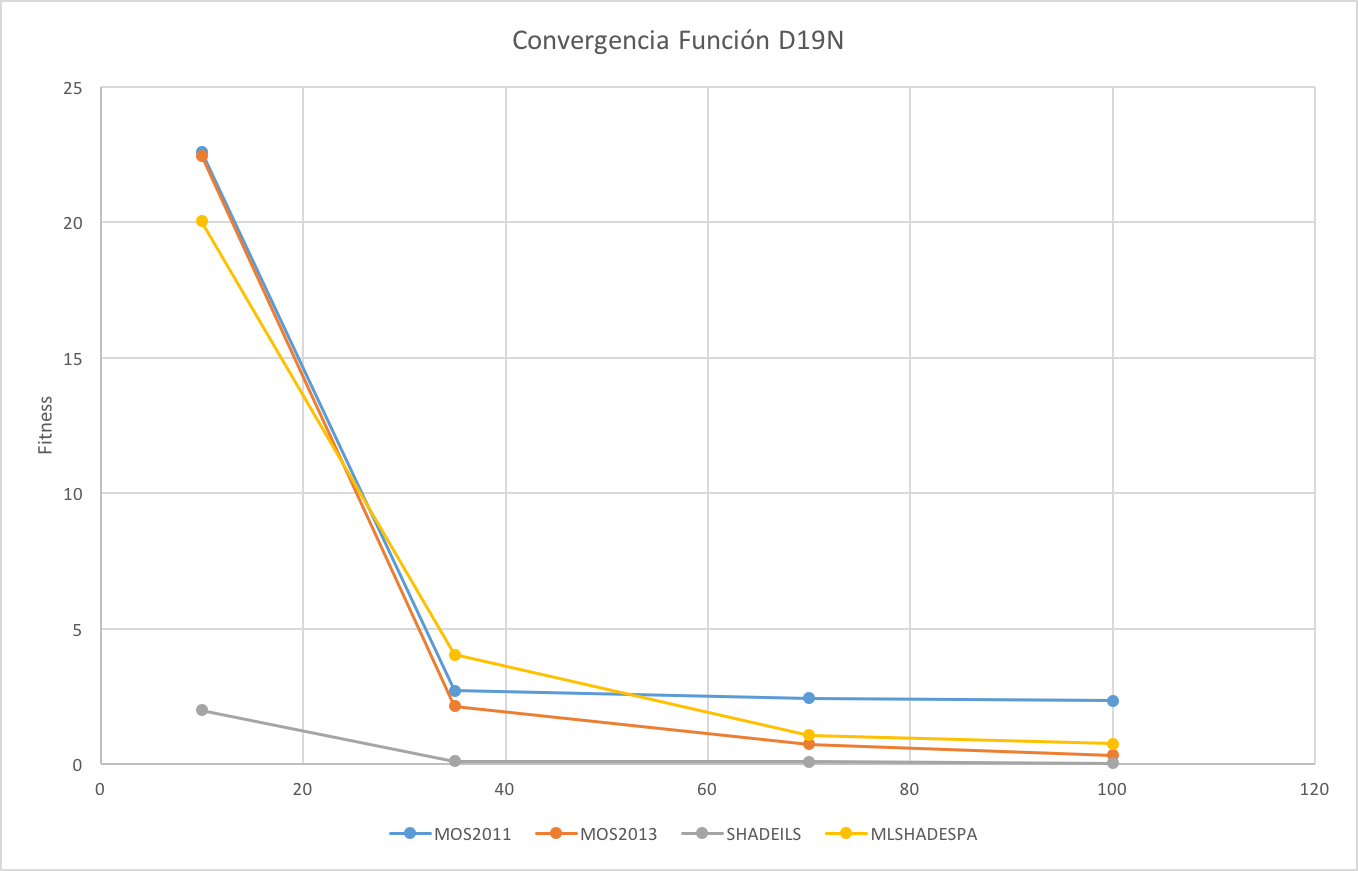
\includegraphics[scale=0.6]{imagenes/ConvergenciaD19N}
	\caption{Convergencia de los 4 algoritmos: problema D19N}
	\label{fig:ConvgD19N}
\end{figure}
%%\input{apendices/paper/paper}
%\input{glosario/entradas_glosario}
% \addcontentsline{toc}{chapter}{Glosario}
% \printglossary
\chapter*{}
\thispagestyle{empty}

\end{document}
